
\documentclass[fleqn, usenatbib]{mnras} 
\usepackage{newtxtext, newtxmath} 	% Required for MNRAS 
\usepackage[T1]{fontenc} 
\usepackage{graphicx}
\usepackage{amsmath}
\usepackage{amssymb}
\usepackage{mathtools}
\usepackage{multicol}
\usepackage{bm}
\usepackage{pdflscape}
\usepackage{natbib}
\usepackage[section]{placeins}
\usepackage{lipsum}
\usepackage{etoolbox} 
\usepackage{tabularx} 
\usepackage{xcolor} 
\usepackage[toc, page]{appendix} 
% \hypersetup{draft} 
% \linespread{1.8} 
\hypersetup{ 
	colorlinks		= true, 
	urlcolor 		= blue, 
	linkcolor 		= blue, 
	citecolor 		= blue 
} 

\newcommand{\ddfrac}[2]{\frac{\displaystyle #1}{\displaystyle #2}} 
\newcommand{\refp}[1]{(\ref{#1})} 
\newcommand{\msun}{\ensuremath{\text{M}_\odot}} 
\newcommand{\persqkpc}{\ensuremath{\text{kpc}^{-2}}} 
\providecommand{\noopsort}[1]{} 
\graphicspath{ {../plots/} } 

\interfootnotelinepenalty = 10000 
\defcitealias{Kroupa2001}{Kroupa} 
\defcitealias{Salpeter1955}{Salpeter} 

\title[Stellar Migration and Chemical Enrichment]{Stellar Migration and 
Chemical Enrichment in the Milky Way Disc: A Hybrid Model} 

\author[J.W. Johnson et al.]{
	James W. Johnson,$^{1}$\thanks{Contanct e-mail: \href{mailto:
	johnson.7419@osu.edu}{johnson.7419@osu.edu}} 
	David H. Weinberg,$^{1, 2, 3}$ 
	Fiorenzo Vincenzo,$^{2}$ 
	Jonathan C. Bird,$^{4}$ 
	\newauthor 
	Sarah R. Loebman,$^{5}$ 
	Alyson Brooks,$^{6}$ 
	Thomas R. Quinn,$^{7}$ 
	Charlotte R. Christensen,$^{8}$ 
	\newauthor 
	et al.?
	\\
	$^{1}$ Department of Astronomy, The Ohio State University, 
	140 W. 18th Ave., Columbus, OH, 43210, USA 
	\\ 
	$^{2}$ Center for Cosmology and Astroparticle Physics (CCAPP), 
	The Ohio State University, 191 W. Woodruff Ave, Columbus, OH, 43210, USA 
	\\ 
	$^{3}$ Institute for Advanced Study, 1 Einstein Dr., Princeton, NJ, 08540, 
	USA 
	\\ 
	$^{4}$ Department of Physics \& Astronomy, Vanderbilt University, 
	2301 Vanderbilt Place, Nashville, TN, 37235, USA 
	\\ 
	$^{5}$ Department of Physics, University of California Merced, 
	5200 North Lake Rd., Merced, CA, 95343, USA 
	\\ 
	$^{6}$ Department of Physics \& Astronomy, Rutgers University, 136 
	Frelinghuysen Rd, Piscataway, NJ, 08854, USA 
	\\ 
	$^{7}$ Department of Astronomy, University of Washinton, Box 351580, 
	Seattle, WA, 98195, USA 
	\\ 
	$^{8}$ Department of Physics, Grinnell College, 1116 8th Ave., Grinnell, 
	IA, 50112, USA 
} 

\date{Accepted XXX; Received YYY; in original form ZZZ} 
\pubyear{2020} 

\begin{document} 
\label{firstpage} 
\pagerange{\pageref{firstpage}--\pageref{lastpage}} 
\maketitle 

\begin{abstract} 
We investigate the impact of stellar migration on galactic chemical evolution 
models, considering a handful of assumptions for the star formation history 
and time-dependence of radial migration based on a zoom-in, hydrodynamical 
simulation of galaxy evolution. When stars migrate with a smooth, continuous 
time dependence, the type Ia supernova rate exhibits significant variability in 
our models. We demonstrate that this is a means with which young, super-solar 
[$\alpha$/Fe] in the solar neighbourhood can arise naturally out of inside-out 
Galaxy growth with stellar migration. We find 
that the observed age-[$\alpha$/Fe] relation is well-fit by an inside-out star 
formation history, while the age-[$\alpha$/H] and age-[Fe/H] relations are 
well-fit by a late starburst model; no one model investigated here fits both 
simultaneously. Our model successfully reproduces the broad nature of the 
[$\alpha$/Fe] distribution at fixed [Fe/H] in a given Galactic region; however, 
an overprediction of the frequency of intermediate [$\alpha$/Fe] stars prevents 
it from explaining the observed results in detail. This suggests 
that inside-out galaxy growth combined with stellar migration, even with a late 
starburst, is not conducive to forming the infamous bimodality as it is 
observed. We postulate that more dramatic evolutionary scenarios (e.g. a 
two-infall model) may be necessary to describe the observed results. In 
conducting this analysis, we developed and made use of newly released features 
in the \texttt{Versatile Integrator for Chemical Evolution} (\texttt{VICE}) 
which are built to handle these models under a wide variety of 
assumptions. \texttt{VICE} is publicly available 
at~\url{https://pypi.org/project/vice}. 
\end{abstract} 

\begin{keywords} 
methods: numerical -- galaxies: abundances, evolution, star formation, stellar 
content 
\end{keywords}

\section{Introduction} 
\label{sec:intro} 
The orbits of stars are not unchanging. While it has been known for some time 
that stars undergo radial migration (e.g.~\citealp*{Wielen1996}; 
\citealp{Roskar2008a,Loebman2011,Minchev2012}), the true impact of this process 
on galactic chemical evolution (GCE) remains under debate. By mixing stellar 
populations which formed in Galactic regions with significantly different 
enrichment histories, in principle the impact could be considerable. While some 
authors argue that radial migration has only a small impact on GCE 
(e.g.~\citealp*{Kubryk2013};~\citealp{Khoperskov2021}), there are others who 
argue the contrary (e.g.~\citealp{Schoenrich2009};~\citealp*{Sharma2020}). 
Aside from the chemodynamical simulations involving N-body integrations 
\citep[e.g.][]{Kubryk2013, Vincenzo2020, Khoperskov2021}, there are to date 
only a handful of GCE models that take this effect into account (e.g. 
\citealp{Matteucci1989, Schoenrich2009};~\citealp*{Minchev2013}; 
\citealp{Sharma2020}). These studies treat the Milky Way as a series of 
concentric annuli, each described by a conventional one-zone GCE model with 
parameters that change from annulus to annulus. In the resultant ``multi-zone'' 
model, stars and gas can migrate between zones under some prescription to 
account for time-dependent mixing processes. We retain such methodology in this 
paper, allowing star particles from a hydrodynamical simulation ran from 
cosmological initial conditions to inform our implemented mixing process; 
\citet{Minchev2013} employ a similar technique. With parameters tuned to 
reproduce certain observed results (e.g. abundance and surface density 
gradients), we can then assess the model predictions to address the following 
question: when combining simple, conventional assumptions about the star 
formation and dynamical histories of the Milky Way, what observed results can 
be replicated? In the present paper, we focus on the following observables: 
metallicity distributions functions (MDFs) and abundance gradients, the 
[$\alpha$/Fe] bimodality, the age-metallicity relation (AMR), and the young, 
$\alpha$-rich population. 
\par 
Stars in the inner regions of the Milky Way tend to be more metal-rich than 
those found in the outskirts~\citep{Nordstroem2004b, Daflon2009, 
Frinchaboy2013, Hayden2014}, with slight variations in quantitative results 
based on what type of stars are considered and what metallicity tracers are 
analysed. Such behavior is also seen in the gas-phase gradients of 
low-redshift spirals (see, e.g., the results from the CHAOS project using HII 
regions;~\citealp{Berg2015, Berg2020}). Using the 12th data release of the 
Apache Point Observatory Galaxy Evolution Experiment (APOGEE), 
\citet{Hayden2015} demonstrate that the observed MDF has a metal-rich mode and 
is skew-negative in the inner galaxy (and conversely, metal-poor and 
skew-positive in the outer galaxy). These variations in the skewness of the 
distributions with Galactocentric radius are usually attribute to the migration 
of metal-rich (metal-poor) stars from smaller (larger) orbital radii. Similar 
arguments are used by~\citet{Sellwood2002} to interpret the results of 
\citet{Edvardsson1993} on scatter in the age-metallicity relation observed in 
the solar neighbourhood. 
\par 
Abundance gradients have been the focus of many studies and are quantified 
rather extensively, but their origin is somewhat up for debate. Applying the 
analytic models of~\citet*{Weinberg2017}, one could argue that the gradient 
arises out of variations in the local gas-phase equilibrium abundance as a 
function of Galactocentric radius. For $\alpha$-elements, the equilibrium 
abundance is determined to first order by their yield and the efficiency of 
outflows in removing metals from the star forming reservoir. With a stronger 
gravitational potential in the inner regions of the Galaxy, one might 
reasonably expect outflows to be weaker there, thereby increasing the 
equilibrium abundance.~\citet{Nidever2014} used such an approach to reproduce 
the width of the [Fe/H] distribution for low-$\alpha$ sequence stars in 
APOGEE. However, recent chemical evolution models have successfully replicated 
the gradient with no outflowing winds at all~\citep[e.g.][]{Minchev2013, 
Spitoni2019a}. This is based on arguments from~\citet{Melioli2008, Melioli2009}, 
\citet*{Spitoni2008}, and~\citet{Spitoni2009} who studied Galactic fountains 
using hydrodynamical simulations and numerical models, finding that ejected 
metals tend to reaccrete to a Galactocentric radius similar to where they 
originated. With this result, some authors argue that such outflows do not 
significantly alter the chemical evolution of a Galactic disc, and that instead 
the gradient arises from the higher normalization of the star formation history 
in the inner Galaxy. 
\par 
Like radial abundance gradients, the reality of the infamous [$\alpha$/Fe] 
dichotomy is well established (in Gaia-ESO:~\citealp{Recio-Blanco2014, 
Rojas-Arriagada2017}; in APOGEE:~\citealp{Nidever2014, Hayden2015, 
Weinberg2019}), but its origin is a topic of intense debate. In general, stars 
in the Milky Way tend to fall in one of two populations - the roughly solar 
[Fe/H], solar [$\alpha$/Fe] stars commonly referred to as the low-$\alpha$ 
sequence, and the high-$\alpha$ sequence made up of sub-solar [Fe/H], 
super-solar [$\alpha$/Fe] stars. Recently explored with more current data by 
\citet{Sharma2020}, the notion that it could in principle arise out of radial 
migration traces back to~\citet{Schoenrich2009}. Applying the analytic models 
of~\citet{Weinberg2017}, an alternative pathway to such abundance patterns is 
by an increase in the strength of outflows at late times. Such an evolutionary 
model would predict a decrease in the equilibrium abundance, forming stars 
along the low-$\alpha$ sequence. This scenario has not yet been explored in 
combination with radial migration. 
\par 
Other authors argue that more dramatic evolutionary events are necessary to 
explain the observed results, such as the two-infall model 
(\citealp*{Chiappini1997, Chiappini2001};~\citealp{Romano2010, Grisoni2017, 
Noguchi2018, Palla2020, Spitoni2016, Spitoni2018}). 
In these models, the high-$\alpha$ sequence forms during the Galaxy's initial 
collapse before feedback processes shut off star formation and expel gas into 
the Galactic halo. Then, this material can cool and reaccrete along with 
additional, metal-poor gas from the intergalactic medium, producing a second 
episode of star formation. The dilution associated with the second accretion 
event lowers the gas-phase Fe abundance at fixed [$\alpha$/Fe], forming stars 
along the low-$\alpha$ sequence.~\citet{Spitoni2019a, Spitoni2020} demonstrated 
using the APOKASC sample~\citep{Pinsonneault2014, SilvaAguirre2018} that such 
models can explain the abundances observed in the solar annulus. Although 
\citet{Spitoni2021} recently extended this model to Galactic regions beyond 
the solar annulus, their model did not account for the mixing of stellar 
populations between regions. Though they invoke~\citet{Kubryk2013} and 
\citet{Khoperskov2021} as arguments that it shouldn't impact their results, 
this nonetheless means that two-infall models have not yet been explored in 
combination with a treatment for stellar migration. 
\par 
Recent cosmological zoom-in simulations have found results qualitatively 
similar to the arguments of~\citet{Spitoni2019a, Spitoni2020, Spitoni2021}. 
Using the Auriga simulation suite~\citep{Grand2017},~\citet{Grand2018} 
demonstrate that an early, accretion induced starburst can populate the 
high-$\alpha$ sequence, followed by low-level, sustained star formation on the 
low-$\alpha$ sequence. In this pathway, there is either a rapid transition 
between the two phases, ensuring the chemical space between the sequences is 
relatively unpopulated, or low-metallicity gas accretion dilutes the star 
forming reservoir at fixed [$\alpha$/Fe], populating the low [Fe/H], low 
[$\alpha$/Fe] portion of the low-$\alpha$ sequence.~\citet{Buck2020b} finds 
the dilution scenario in the NIHAO simulation suite as well~\citep{Wang2015, 
Buck2020a}. Although the~\citet{Spitoni2021} model did not implement mixing of 
stellar populations, these studies using hydrodynamical simulations would 
suggest pathways qualitatively similar to their two-infall model. 
\par 
Contrary to this scenario,~\citet{Clarke2019} demonstrate that star formation 
proceeded in clumps in an SPH simulation using GASOLINE~\citep*{Wadsley2017}. 
These clumps self-enrich, forming stars on the high-$\alpha$ sequence due to 
the perturbed ratio of core collapse to type Ia supernova rates within the 
star forming regions. The more spatially extended, smooth star formation 
populates the low-$\alpha$ sequence. Suffice it to say that there are no 
shortage of models which reproduce the dichotomy, but only those done with 
hydrodynamical simulations and a handful of others 
\citep[e.g.][]{Schoenrich2009, Minchev2013, Sharma2020} have taken into account 
stellar migration. 
\par 
Besides abundance gradients and the [$\alpha$/Fe] dichotomy, another 
observable of interest in this paper is the age-metallicity relation (AMR): the 
correlation between stellar ages and metallicities. The observed AMR in the 
solar neighbourhood is known to exhibit considerable intrinsic scatter 
\citep{Edvardsson1993}; this is usually attributed to radial migration of 
metal-rich (metal-poor) stars from smaller (larger) Galactocentric radii 
\citep{Sellwood2002, Haywood2008, Roskar2008b, Schoenrich2009}. 
In the solar neighbourhood,~\citet{Feuillet2018} reveal that super-solar 
metallicity stars are statistically older than solar metallicity stars (see 
their Fig. 3). This contrasts with the predictions of simple one-zone models of 
GCE where enrichment proceeds alongside star formation, yielding a monotonic 
AMR~\citep[e.g.][]{Andrews2017, Weinberg2017}. Although one-zone models of 
starbursts can predict a non-monotonic AMR due to the effect of dilution 
\citep{Johnson2020}, by construction they do not predict multiple abundances at 
fixed age as~\citet{Feuillet2018} reports. Using the~\citet{Weinberg2017} 
analytic models,~\citet{Feuillet2018} argues that this is a consequence of 
radial migration. For a smooth star formation history, the youngest stars at a 
given radius will have compositions reflective of the local equilibrium 
abundance; only stars born at different radii will have different compositions, 
and only the old ones will have had time to migration to the solar annulus. 
\par 
While the presence of old-metal rich stars in the solar annulus is peculiar 
because they are at odds with one-zone models of chemical evolution, the 
presence of young, $\alpha$-rich stars is interesting for the same reason. 
For a smooth star formation history, the delayed nature of type Ia supernovae 
and their Fe production cause [$\alpha$/Fe] to decrease with time, predicting 
an age-[$\alpha$/Fe] relation that should increase monotonically with stellar 
age. However, these~$\sim$few Gyr old stars with [$\alpha$/Fe]~$\approx$~+0.1 - 
0.2 stars have been found using stellar ages estimated from carbon-to-nitrogen 
ratios~\citep{Martig2016}, isochrone matching~\citep{Feuillet2018, 
Feuillet2019}, and with the asterosesmic ages of the original APOKASC catalog 
\citep{Chiappini2015, SilvaAguirre2018, Pinsonneault2014}. 
\citet{SilvaAguirre2018} demonstrate that these stars have kinematics similar 
to the rest of the high-$\alpha$ population, postulating that they may be 
the consequence of stellar mergers or mass transfer events, making truly old 
stars simply appear younger. In a sample of 51 young, $\alpha$-enhanced red 
giant stars,~\citet{Hekker2019} conclude that a portion of these stars have 
carbon-to-nitrogen ratios consistent with mass transfer events, but that this 
cannot account for the entire population. This suggests that the remaining 
stars are either truly young or the result of mergers on the main sequence. 
If not, then a theoretical explanation for the origin of these stars remains 
a mystery. 
\par 
Alternatively, a recent starburst event could have produced these stars. 
\citet{Mor2019} infer a factor of~$\sim$2 enhancement in the star formation 
history (SFH) of the Milky Way~$\sim$2 Gyr ago by comparing population 
synthesis models to observed stellar luminosity functions and colour-magnitude 
diagrams from Gaia data~\citep{GaiaDR2}.~\citet{Isern2019} reach similar 
conclusions by modeling the white dwarf luminosity function in the solar 
neighbourhood with Gaia parallaxes. Motivated by these results, 
\citet{Johnson2020} demonstrate using one-zone chemical evolution models that 
a recent starburst of this nature can produce similarly young,~$\alpha$-rich 
stars. However, the caveat to this interpretation is that the starburst must be 
sufficiently localized such that the resultant stellar populations remain 
outliers from an otherwise monotonically increasing age-[$\alpha$/Fe] relation. 
\par 
The impact of such evolutionary histories combined with stellar migration is, 
to our knowledge, yet unexplored in the literature. A viable model for the 
detailed enrichment history of the Milky Way would simultaneously explain all 
of these observed results and their variations between Galactic regions, while 
also taking into account effects like mixing and observational systematics. On 
top of this, it must self-consistently calculcate enrichment rates from adopted 
nucleosynthetic yields and the SFH. In this paper, we aim to 
assess the extent to which conventional assumptions about the evolutionary 
history of the Milky Way can account for these results, entertaining a 
handful of assumptions describing the SFH and time-dependence of stellar 
radial migration. 
\par 
Motivated by the general result that galaxies grow in radius with time 
(i.e. ``inside-out'' growth;~\citealp{Bird2013}), our base-line model has a 
star formation history (SFH) whose e-folding timescales grow with 
Galactocentric radius. Based on the findings of~\citet{Mor2019} and 
\citet{Isern2019}, we also construct models in which a late starburst is 
imposed atop the inside-out SFH. In one model, this starburst occurs in all 
annuli, and in another, loosely informed by the findings of 
\citet{Vincenzo2020} suggesting such a radial dependence to accretion, it 
occurs only at~$\geq$6 kpc. We also construct a model in which the SFH is 
constant at a given Galactocentric radius; these models are interesting from a 
theoretical perspective in that they quantify the impact of stellar migration 
without the effects of a time-dependent SFH. 

\section{Methods} 
\label{sec:methods} 
To fulfill the goals of this paper, we develop and make use of newly released 
features within the~\texttt{Versatile Integrator for Chemical Evolution} 
(\texttt{VICE};~\citealp{Johnson2020}). These features are designed to handle 
models such as these with a wide range of flexibility. We reserve a description 
of~\texttt{VICE}'s migration algorithm and our simulation parameters for~\S 
\ref{sec:methods:migration}, first describing our sample of star particles from 
the hydrodynamical simulation. 
\par 
Although we make use of a hydrodynamical 
simulation to drive stellar migration, we do~\textit{not} make use of its SFH. 
While our study employs similar techniques as~\citet{Minchev2013}, our differs 
in this subtle aspect. An alternative to modeling radial migration based on a 
hydrodynamical simulation is to invoke dynamical arguments; 
\citet{Schoenrich2009} and~\citet{Sharma2020} take such an approach. This 
method, however, introduces free parameters which then require fitting to 
data. An advantage of our technique is that there are no free parameters 
introduced to the model; furthermore, it's unclear the extent to which the fit 
biases the model into agreement with parts of the data not involved in the 
fitting process. The dynamical history of a hydrodynamical simulation is also 
motivated by first principles in that it models gravitational interactions via 
an N-body integration. The primary disadvantage of this approach is a 
consequence of the lack of free parameters - the model is rigid, and we cannot 
explore slight variations. However, in principle one could compare the 
predictions made by our chemical evolution models when ran using different 
hydrodynamical simulations. We emphasize that a hydrodynamical simulation 
\textit{only} informs the mixing processes in our models, and there is no 
N-body integration involved in our models aside from that which was used to run 
the hydrodynamical simulation in the first place. 

\subsection{The Hydrodynamical Simulation} 
\label{sec:methods:h277} 
In this paper we make use of star particles from the~\texttt{h277} simulation 
\citep{Christensen2012, Zolotov2012, Loebman2012, Loebman2014, Brooks2014}. 
Recently employed to study the stellar age-velocity relationship, a synopsis of 
its detailed simulation parameters and cosmological model can found in~\S 2 of 
\citet{Bird2020}. We do not include any discussion of these details here, 
instead focusing on how we vet the sample of star particles for use in our 
chemical evolution models. 
\par 
It is of particular important to have accurately measured formation radii for 
each star particle that we use in our analysis.~\texttt{h277} did not record 
the exact birth radius of each star particle; however, each star particle does 
have an accurate age at each snapshot. Since stellar orbits are unlikely to 
change significantly in an adequately short time interval, the radii of 
sufficiently young stars in their first snapshot are reasonable approximations 
of their birth radii. We therefore restrict our sample to those with an age at 
first snapshot of~$\leq$~150 Myr, and adopt their Galactocentric radius at that 
time as their birth radius. We have also conducted this analysis with a maximum 
age at first snapshot of 50 Myr, and found similar results, suggesting that 
these time intervals are short enough to not impact our conclusions. In 
practice, we find that 150 Myr also provides with an adequately large number of 
star particles to sample from. Of the star particles that remain after imposing 
this cut, the oldest one is 12.26 Gyr old at the present day. Our model can 
only apply on timescales as long as or shorter than the full range of ages of 
the sample of star particles; we therefore subtract 1.5 Gyr from the formation 
times of all star particles, allowing~$T$~= 0 in our models to correspond to 
$T$~= 1.5 Gyr in~\texttt{h277}. As a consequence, our disc models trace the 
chemical evolution of the Galaxy out to a lookback time of~$\sim$12.2 Gyr, or a 
redshift of~$z \approx$~3, placing the onset of star formation at that time. 
\par 
We further restrict our sample of star particles to only those with both 
formation and final radii of~$R_\text{gal} \leq$~20 kpc, and to have formed 
within~$\left|z\right|\leq$~3 kpc of the disc midplane. These criteria ensure 
that we're only using star particles which formed in-situ. While it's possible 
that some star particles formed in a dwarf galaxy as it was infalling, a 
scenario which would satisfy these requirements, these star particles are few 
in number, and are only relevant at large~$R_\text{gal}$ and high ages - a 
region of parameter space where few stars form anyway. 
\par 
Based on a kinematic decomposition performed on the present-day phase space 
distribution of the~\texttt{h277} star particles, we include all those with 
bulge, pseudobulge, and disc-like kinematics, excluding halo stars. While we're 
not modeling the evolution of the bulge here, these star particles are 
overwhelmingly located at~$R_\text{gal}\leq$~3 kpc at the present day anyway; 
here we're much more interersted in~$R_\text{gal}\geq$~3 kpc since we're 
modeling the evolution of the disc. These cuts yield a sample of 3,000,556 star 
particles from~\texttt{h277}. 
\par 
\texttt{h277} had a transient bar during its evolution, but does not have one 
at~$z$ = 0 ({\color{red} citation?}). This is a noteworthy difference between 
our model and that of~\citet{Minchev2013}, and by extension the 
\citet*{Minchev2014} and~\citet{Minchev2017} studies which use it as well, 
because they selected a hydrodynamical simulation of a galaxy specifically so 
that it would have a strong bar at~$z$ = 0; the transient bar in~\texttt{h277} 
was not strong. This could mean that the dynamical 
history of our model Galaxy does not reflect that of~\citet{Minchev2013} and 
perhaps the Milky Way itself. However, the difference is likely within the 
uncertainties of the current understanding of the Milky Way's dynamical 
history. Although an investigation on the impact of bar evolution on stellar 
migration and thus chemical evolution is outside the scope of this paper, it is 
an interesting question which can be probed by simply swapping the 
\texttt{h277} data within~\texttt{VICE} for another simulation, then rerunning 
our numerical models and comparing the results. 

% fig 1 
\begin{figure*} 
\centering 
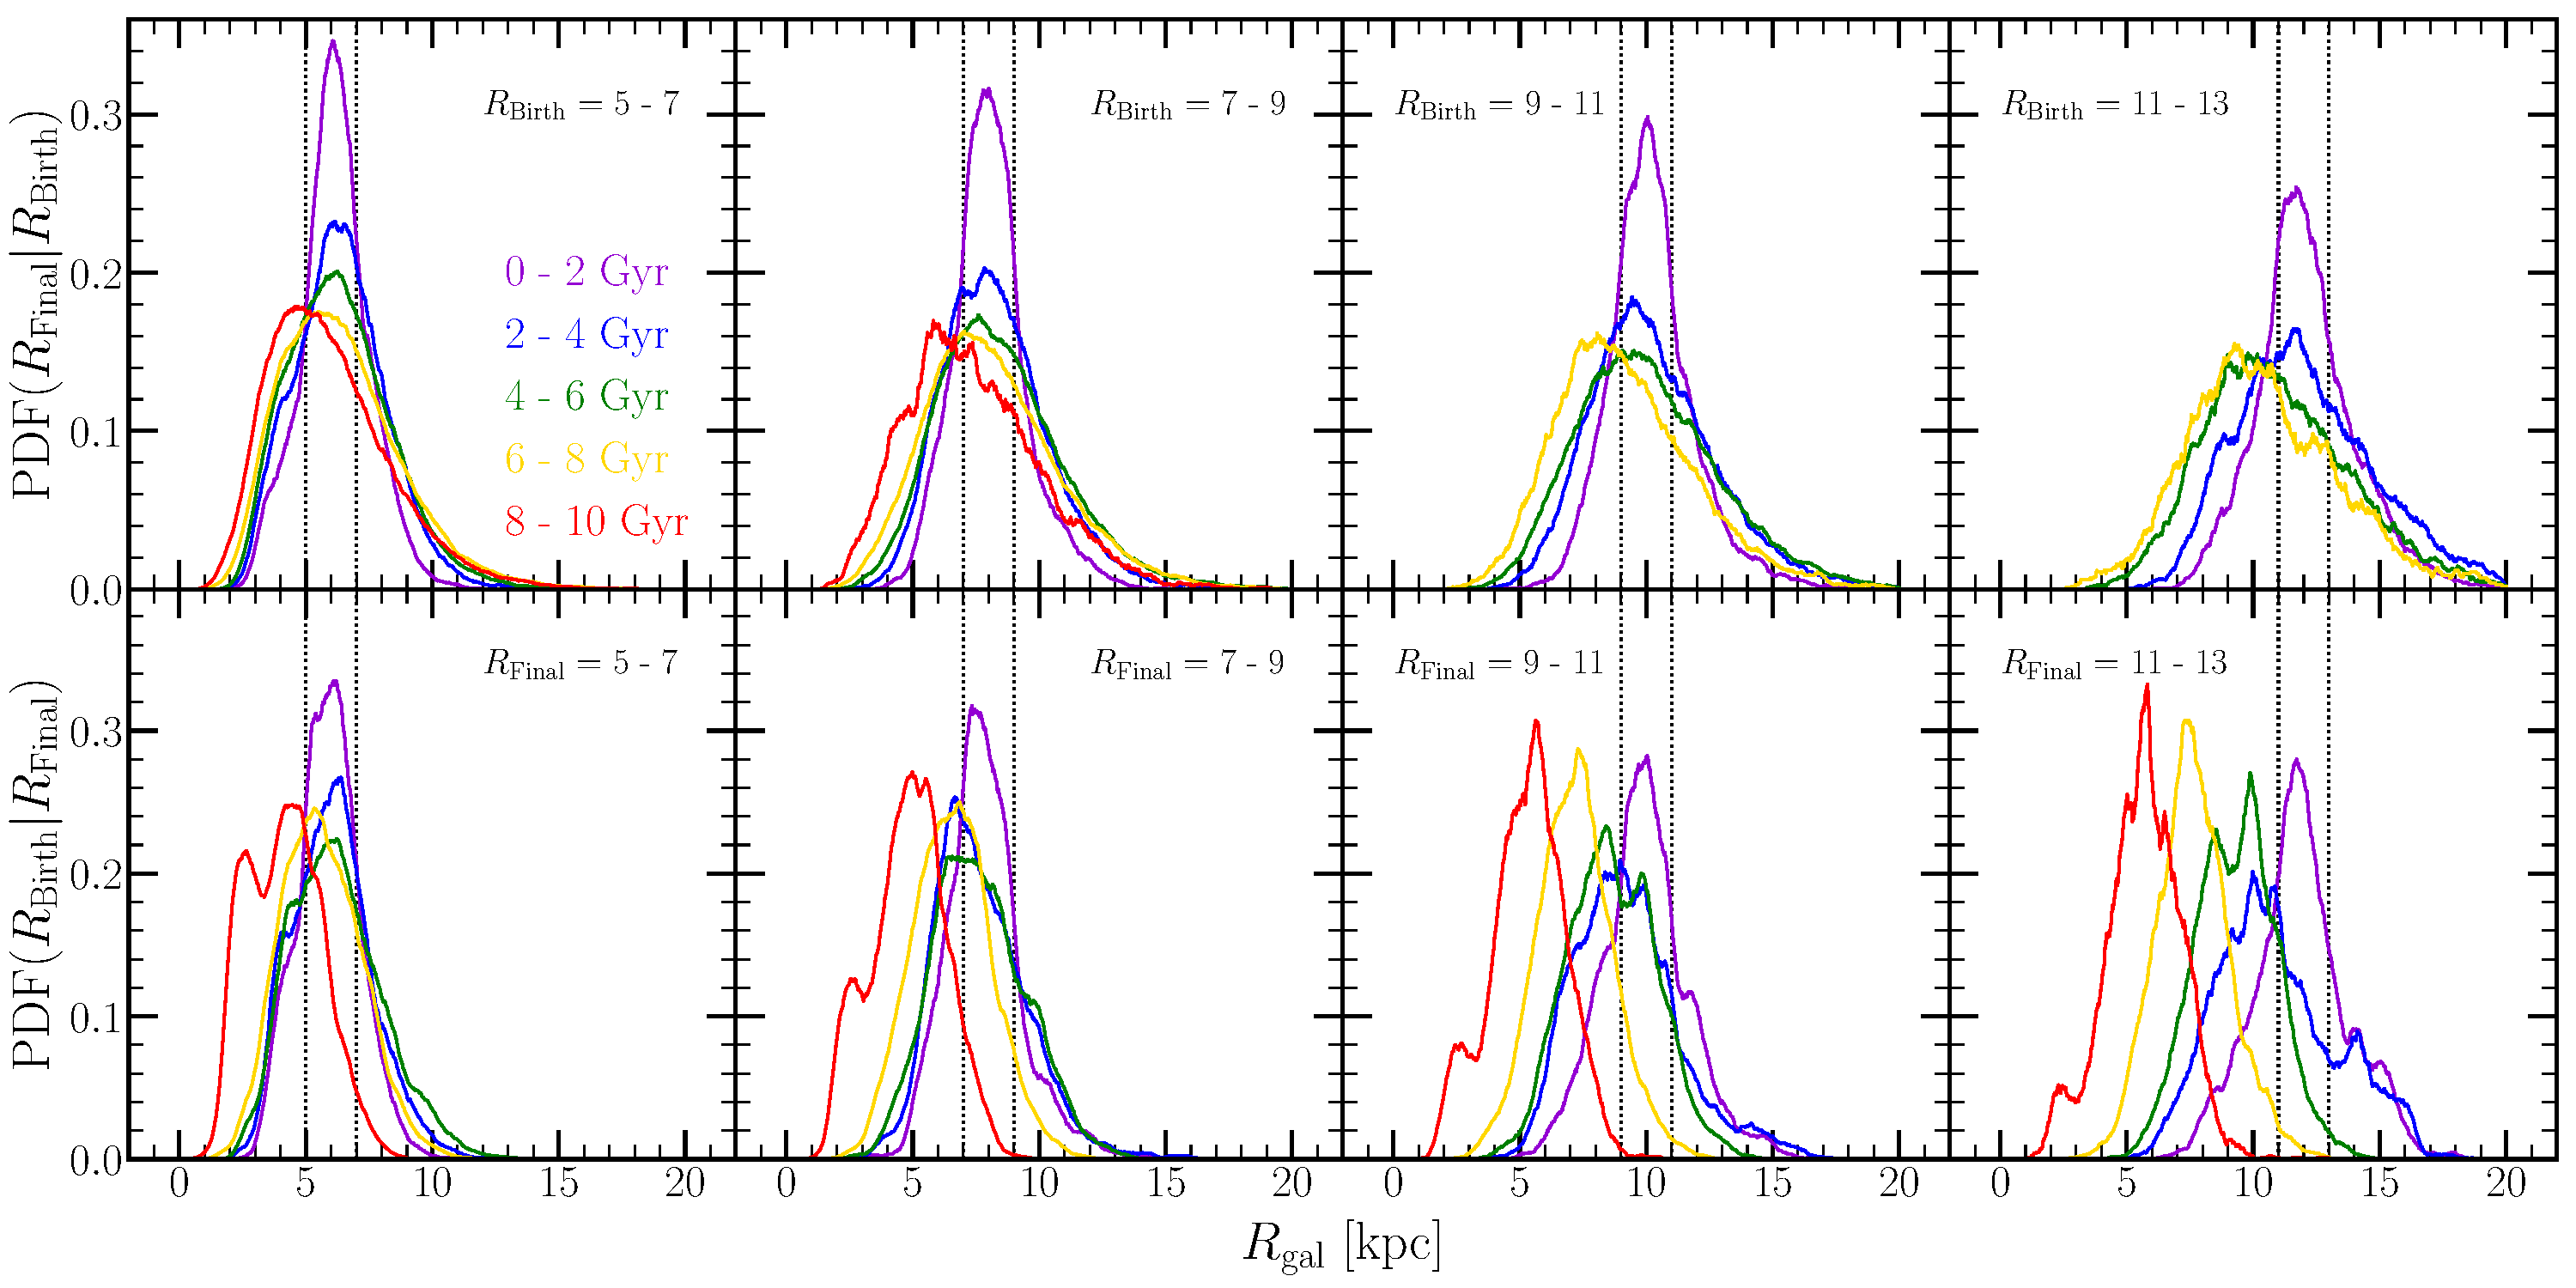
\includegraphics[scale = 0.32]{decomposition.pdf} 
\caption{Radial distributions of our star particles from 
\texttt{h277}. In the top row, we show distributions of~\textit{final} radius 
in bins of birth radius and age, and in the bottom row, we show distributions 
of~\textit{birth} radius in bins of final radius and age. Each bin in 
Galactocentric radius is shown in its own panel, denoted in text at the top of 
each panel and by vertical black dashed lines. We colour-code the distributions 
according to the age of the star particles, denoted by the legend in the upper 
left panel. We smooth all distributions with a box-car width of 0.5 kpc to 
improve clarity. We omit the distributions for 8 - 10 Gyr old stars born in the 
9 - 11 and 11 - 13 kpc bins due to an insufficient number of star particles 
with which to calculate the distribution. } 
\label{fig:h277_decomposition} 
\end{figure*} 

In the top row of Fig.~\ref{fig:h277_decomposition}, we plot the distributions 
of final radius in bins of birth radius and age for our sample of star 
particles. Conversely, the bottom rows distributions of birth radii in bins of 
final radius and age. Focusing on the top row of panels, we note that for star 
particles born at any radius and time, the distribution of final radius is 
still peaked near the birth radius, but moves slightly inward with increasing 
age. The tails of the distributions toward larger~$R_\text{gal}$ are nearly 
age-independent, while the tails toward smaller~$R_\text{gal}$ are not. This 
suggests that radial migration inward and outward occur on different timescales 
in~\texttt{h277}, specifically that inward migration is slower than outward 
migration. By extension, this suggests that the two may be tied to different 
physical processes. In a cosmological simulation,~\citet{Roskar2008a} 
demonstrate that resonant scattering at corotation causes stars to move 
outward and gas to move inward. It's possible that stellar migration inward has 
different origins. 
\par 
Focusing on the bottom row of panels in Fig.~\ref{fig:h277_decomposition}, we 
note that the mode of the birth radius distributions show a stronger dependence 
on age than the mode of the final radius distributions. At any Galactocentric 
radius at the present day, the youngest stars are overwhelmingly born at 
comparable radii, while the oldest stars are overwhelmingly born at smaller 
radii. This is most noticeable in at large~$R_\text{gal}$. The differences 
between the two can be understood by considering the steep nature of the radial 
gradient in stellar surface density. Take for example the 8 - 10 Gyr age bin in 
both~$R_\text{Birth}$ = 5 - 7 kpc and~$R_\text{Final}$ = 11 - 13 kpc bins (i.e. 
the red curves in the top-left and bottom-right panels). For these old stars 
born at 5 - 7 kpc, 11 - 13 kpc is far down the tail of the~$R_\text{Final}$ 
distribution, and yet 5 - 7 kpc is the mode~$R_\text{Birth}$ of all old stars 
presently at these radii. This implies that even though a plurality of 8 - 10 
Gyr old stars with~$R_\text{Final}$ = 11 - 13 kpc were born at 5 - 7 kpc, they 
account for only a small fraction of the stars with similar birth radii. This 
is only possible if there are many more stars born at small~$R_\text{gal}$ than 
large~$R_\text{gal}$, implying a stellar surface density which decreases as a 
strong function of Galactocentric radius. This is known to be the case 
\citep[e.g.][]{Bland-Hawthorn2016}. 
\par 
We also note that the top row of Fig.~\ref{fig:h277_decomposition} demonstrates 
that the number of stars which migrated inward and outward are comparable in 
\texttt{h277}. In fact, taking~$\left|\Delta R_\text{gal}\right| \geq$~500 pc 
between birth and final radii as the criterion for migration inward or outward, 
we indeed find as global percentages in our sample that 27\% migrated inward, 
29\% migrated outward, and the remaining 44\% stayed near their birth radius. 
Furthermore, these distributions contain some information on the timescales of 
radial migration. In all bins of birth radius, a good first-order estimate of 
the probability density that a star has a final radius in the same bin is 
$\sim$0.3. With bins in birth radius of 2 kpc, this suggests that only 
$\sim$60\% of stars remain in their birth radius bin by the time their~$\sim$2 
Gyr old. and the remaining~$\sim$40\% have migrated already. If the type Ia 
supernova delay-time distribution (SN Ia DTD) is a~$t^{-1.1}\approx t^{-1}$ 
power-law as suggested by observational results~\citep[e.g.][]{Maoz2012, 
Maoz2017}, then we expect similar numbers of SN Ia events to occur with delay 
times between 1 and 10 Gyr as we do between 100 Myr and 1 Gyr. With such an 
extended DTD, and the timescales for migration implied by Fig. 
\ref{fig:h277_decomposition}, its possible that SN Ia progenitors can migrate 
significant distances before exploding. Indeed, in the ASAS-SN bright SN 
catalog,~$\sim$10\% of SNe are seen at >10 kpc from their host galaxies 
\citep{Holoien2019}. While this catalog is for~\textit{all} supernovae seen by 
ASAS-SN, the majority of SN events are type Ia anyway. Based on this, it's 
reasonable to expect that the migration of nucleosynthetic may proceed 
alongside stellar migration. This effect has largely been neglected by GCE 
studies to date on the grounds that radial migration is a slow process, and 
thus the majority of nucleosynthesis should occur near a star's birth radius 
(e.g.~\citealp{Minchev2013}, and in the application of the 
\citealt{Weinberg2017} analytic models in~\citealt{Feuillet2018}). However, 
with the realization that the SN Ia duty cycle is also a slow process due to 
the long tail of the DTD, its possible that stellar migration and SN Ia occur 
on similar timescales. Therefore, we relax this assumption in the present 
paper. We discuss the application of the~\texttt{h277} star particle data to 
our model for radial migration and the time dependence thereof in the next 
section. 

\subsection{Radial Migration} 
\label{sec:methods:migration} 
As in previous studies~\citep[e.g.][]{Schoenrich2009, Minchev2013, Sharma2020}, 
in this paper we model the Milky Way as a series of concentric annuli with a 
uniform width~$\Delta R_\text{gal}$. To run numerical simulations of these 
models, we develop and make use of~\texttt{VICE}'s~\texttt{milkyway} object, 
designed specifically for such an approach. The~\texttt{milkyway} object is a 
subclass of a more general object named~\texttt{multizone}; at its core a 
\texttt{multizone} object is an array of~\texttt{singlezone} objects, which are 
designed to handle one-zone models of GCE and were the focus of 
\citet{Johnson2020},~\texttt{VICE}'s initial release paper. The 
\texttt{multizone} object affords users full control over which zone any 
individual stellar population is in at all timesteps following its formation as 
well as the ability to move gas between any two zones with any time dependence. 
In principle this should allow for arbitrarily complex zone configurations and 
migration prescriptions. The \texttt{milkyway} object is a user-friendly 
extension of this which enforces an annular zone configuration as we take here. 
As defaults, it adopts the stellar migration model detailed in this section and 
our star formation law discussed in~\S~\ref{sec:methods:sfe}. 
\par 
As in hydrodynamical simulations, stars in~\texttt{VICE} are stand-ins for 
entire stellar populations. They're said to be in a given zone if their radius 
is between the inner and outer edges of the annulus. At all times, their 
nucleosynthetic products and returned envelopes are placed in the ISM of the 
annulus that they are in~\textit{at that time}. Where hydrodynamical and 
N-body simulations of Galaxy evolution tend to use star particles of a fixed 
mass, however,~\texttt{VICE} forms a fixed number of stellar populations per 
zone per timestep, and allows their masses to vary to account for variations 
in the star formation rate (SFR). The mass of stars formed in a given zone is 
divided evenly among the stellar populations that form in a given zone and 
timestep. 
\par 
The final radius of a stellar population is then determined based on the birth 
and final radii of star particles in a hydrodynamical simulation, for which 
we've taken~\texttt{h277} in this paper (see discussion in~\S 
\ref{sec:methods:h277}). Describing the Galaxy as a series of concentric 
annuli,~\texttt{VICE}'s~\texttt{milkyway} object assumes stellar populations 
are born at the centres of each annulus. For a stellar population born at a 
time~$T$ and Galactocentric radius~$R_\text{gal}$, it first searches for star 
particles from~\texttt{h277} that formed at~$T \pm$~250 Myr and~$R_\text{gal} 
\pm$~250 pc. It then randomly selects a star particle from this subsample with 
no bias to act as an~\textit{analog}. This stellar population then assumes the 
change in orbital radius~$\Delta R_\text{gal}$ of its analog at face value, 
and moves from its birth radius to the implied final radius at~$T$ = 12.2 Gyr 
with an assumed time dependence. If no candidate analogs are found, 
\texttt{VICE} widens the search to~$T \pm$~500 Myr and~$R_\text{gal} \pm$~500 
pc. If still no analog is found, then it finds the star particle 
with the smallest difference in birth radius still within a birth time of 
$T \pm$~500 Myr, and assigns it as the analog. 
While this prescription allows stellar populations to be assigned analogs with 
significantly different birth radii, this is only an issue for small~$T$ and 
large~$R_\text{gal}$ where there are few star particles from~\texttt{h277}, 
and where few stars form in nature anyway due to the inside-out growth of 
galaxies~\citep{Bird2013}. Furthermore, due to the similarity of the histograms 
in the top row of Fig.~\ref{fig:h277_decomposition}, we expect taking 
$\Delta R_\text{gal}$ from a star particle which formed at a similar time but 
different birth radius in these instance to be accurate enough for our 
purposes. 
\par 
Our models assume that the Galaxy is vertically and azimuthally well-mixed, and 
that the radial direction is the only one in which there are significant 
differences in composition. That is, each annulus extends from the disc 
midplane at~$z$ = 0 to~$z = \pm \infty$, and whether or not a star particle is 
in a given annulus does not depend on~$z$ at all. In fact, this information is 
\textit{not} used in integrating our models with~\texttt{VICE}. Instead, we 
simply assume that each stellar population in our models are located at the 
present day~$z_\text{final}$ of its assigned analog. Furthermore, when an 
\texttt{h277} star particle is assigned as an analog, it is~\textit{not} 
thrown out of the sample of candidate analogs, in theory allowing a star 
particle to act as an analog for multiple stellar populations. This is a 
subtle difference between the~\citet{Minchev2013} model and ours; where we 
assign star particles to stellar populations for which~\texttt{VICE} then 
calculates a stellar mass and composition based on an assumed SFH, the 
\citet{Minchev2013} uses a chemical evolution model to assign compositions to 
star particles. 

% fig 2 
\begin{figure} 
\centering 
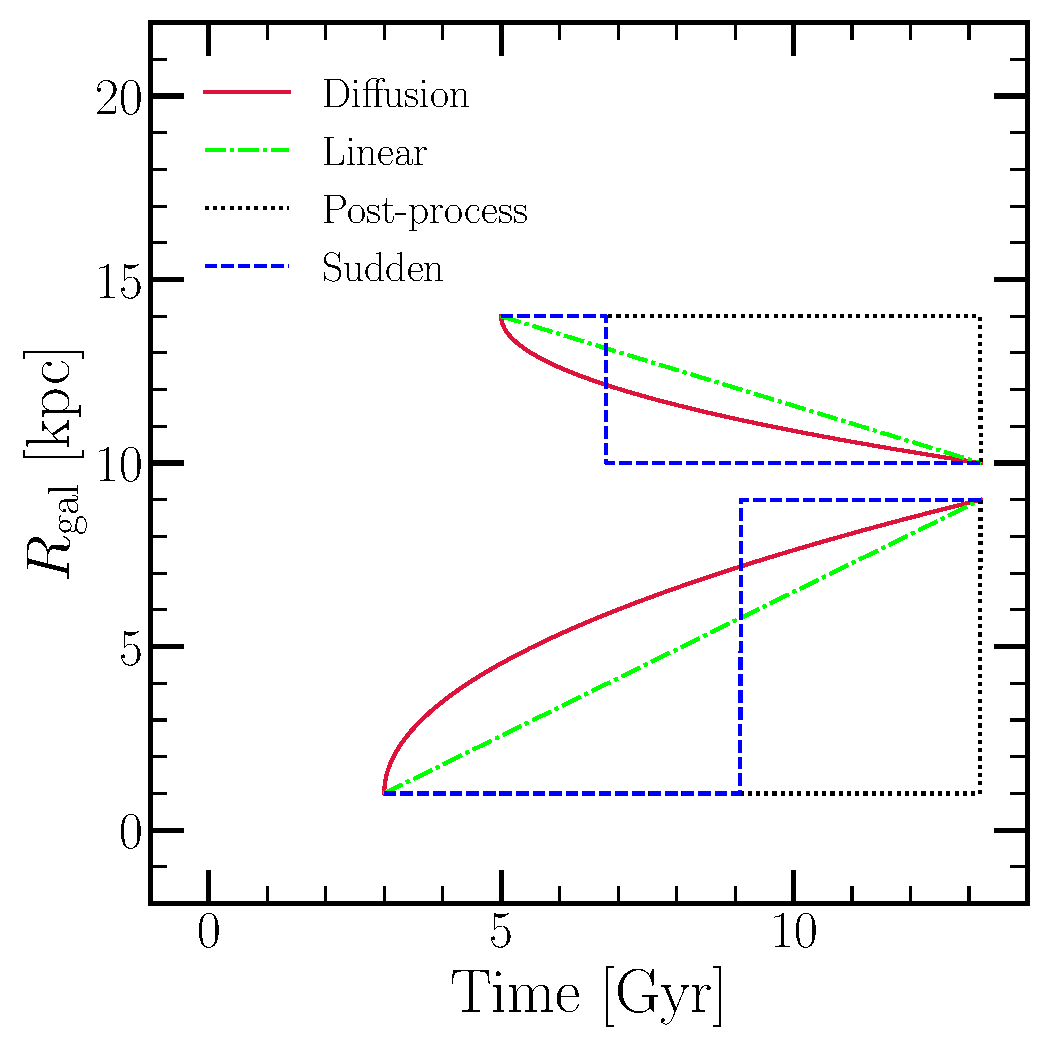
\includegraphics[scale = 0.45]{migration.pdf} 
\caption{A diagram illustrating how Galactocentric radius changes with time for 
two stellar populations under our migration schema: diffusion (crimson, solid), 
linear (lime, dot-dashed), post-process (black, dotted), and sudden (blue, 
dashed). Here the initial and final radii and birth times are chosen at random 
for illustrative purposes. With the initial and final Galactocentric radii of 
a stellar population, its birth time, and one of these assumptions regarding 
the time-dependence of radial migration, the Galactocentric radius at all times 
is known. } 
\label{fig:migration_schema} 
\end{figure} 

With a known birth radius and time from our GCE model and an implied 
$\Delta R_\text{gal}$ from a stellar population's assigned analog, the final 
radius is known and the only missing piece of information is the 
time-dependence with which it moves there. In the present paper we consider 
four parameterized assumptions to describe this, each of which are illustrated 
conceptually in Fig.~\ref{fig:migration_schema}. 
\begin{itemize} 
	\item \textbf{Post-Processing}: Stars stay where they are born until the 
	final timestep, at which point they instantly migrate to their final 
	radius. This retains the assumption that stars do not contribute to 
	nucleosynthesis beyond their birth radius as employed in previous studies 
	\citep[e.g.][]{Minchev2013}. In this scenario, each annulus is treated as 
	a one-zone model independent of all other zones. We illustrate this case 
	with a black dotted line in Fig.~\ref{fig:migration_schema}. 

	\item \textbf{Sudden}: A random number is drawn from a uniform distribution 
	between a stellar population's time of birth and the present day. That time 
	is taken to be the time of instantaneous migration to the present-day 
	annulus. This emulates a scenario in which a single dynamical interaction 
	changes a star's orbital radius, and be thought of mathematically as a 
	time-dependent extension of the post-processing scenario. We illustrate 
	this case with a blue dashed line in Fig.~\ref{fig:migration_schema}. 

	\item \textbf{Diffusion}: Stars move to their final radii in a continuous, 
	time-dependent manner in this case. So named because it corresponds to a 
	scenario in which angular momentum diffuses via a random walk, under this 
	assumption, the mean displacement of stars that migrate similar distances 
	would scale with~$\sqrt{\text{age}}$. This is our 
	fiducial migration model, and we present results with this assumption 
	unless otherwise noted. This is qualitatively similar to 
	\citet{Frankel2018, Frankel2020}, who also model radial orbit migration 
	with a~$\sqrt{\tau}$ dependence. We illustrate this case with a red solid 
	line in Fig.~\ref{fig:migration_schema}. 

	\item \textbf{Linear}: A simple variation of the diffusion model in which 
	the migration to the final radius scales linearly with age rather than with 
	$\sqrt{\text{age}}$. There is no physical motivation for this model other 
	than mathematical ease, but together with the diffusion model it 
	constitutes a test of how sensitive our conclusions are to the 
	time-dependence of stellar migration. We illustrate this case with a 
	green dot-dashed line in Fig.~\ref{fig:migration_schema}. 
\end{itemize} 
In all models, we neglect radial gas flows~\citep{Lacey1985, Bilitewski2012}, 
instead focusing on these simple assumptions describing how orbital radii 
change with time. While such an investigation would be an interesting extension 
of our study, we reserve it for future work. 
\par 
We emphasize that there is~\textit{no} N-body integration employed in our 
models aside from that which ran the~\texttt{h277} simulation. Furthermore, we 
use our sample of analog star particles from it~\textit{only} in determining 
$\Delta R_\text{gal}$ of each of our model stellar populations (see discussion 
in~\S~\ref{sec:methods:h277}). While~\texttt{h277} had its own SFH and chemical 
enrichment history, we make use of neither of these components here; rather, 
these are exactly what we seek to explore variations of. We acknowledge that 
stellar migration is often formulated using the processes ``blurring'' and 
``churning'', referring to a star's epicyclic motions and changes in the 
guiding center of its orbit~\citep[e.g.][]{Sellwood2002, Schoenrich2009, 
Minchev2011}; migration can also occur due to the overlap of spiral arm and 
bar resonances in the disc~\citep{Minchev2011}. We refrain from discussion of 
this approach here, because our models do not make use of such methodology. In 
the present paper, the orbital radii at all times are calculated and assumed at 
face value given one of the four assumptions detailed in the bullet list above. 
\par 


\subsection{Nucleosynthetic Yields, Outflows, and Recycling} 
\label{sec:methods:yields} 
Nucleosynthesis proceeds in our models according to~\textit{fractional net} 
yields, as required by~\texttt{VICE}. That is, our yields quantify the mass 
of some element~$x$ ejected to the interstellar medium (ISM) in units of the 
progenitor stellar population's total initial mass, and only accounts for 
\textit{newly produced} nucleosynthetic material.~\texttt{VICE} takes into 
account the return of previously produced nucleosynthetic products with a 
separate implementation. In the present paper, we focus our analysis on 
alpha and iron-peak elements, taking oxygen (O) and iron (Fe) as the 
representative cases. The dominant enrichment channels of 
interest in our models are thus core collapse and type Ia supernovae 
\citep{Johnson2019}. Though we choose O and Fe, we expect 
similar results to be found for other alpha (e.g. Ne, Mg, Si) and iron-peak 
elements (e.g. Mn, Ni, Co), with purely quantitative differences reflective of 
the relative yields between elements. 
\par 
Enrichment from core collapse supernovae (CCSNe) happens immediately following 
the formation of progenitor stars in~\texttt{VICE}. This is an adequate 
approximation, because the lifetimes of massive stars are short compared to 
the relevant timescales for galaxy evolution. For the most massive stars, the 
lifetimes are comparable to the timestep size we adopt in this paper anyway. 
This assumption implies a linear relationship between the CCSN enrichment 
rate and the SFR: 
\begin{equation} 
\dot{M}_x^\text{CC} = y_x^\text{CC}\dot{M}_\star 
\end{equation} 
where~$y_x^\text{CC}$ is the CCSN yield of some element~$x$. Physically, this 
quantity represents the mass of an element~$x$ ejected to the interstellar 
medium (ISM) from all CCSNe events associated with a stellar population in 
units of the stellar population's initial mass. For example, if 
$y_x^\text{CC} = 0.01$, a hypothetical 100~\msun~stellar population would 
add 1~\msun~of~$x$ to the ISM immediately. This procedure neglects the mass 
that would be lost to outflows, which like recycling, have a separate 
implementation in~\texttt{VICE}. In this paper, we adopt~$y_\text{O}^\text{CC}$ 
= 0.015 and~$y_\text{Fe}^\text{CC}$~= 0.0012 from~\citet{Johnson2020}, who 
in turn adopt these values from~\citet{Weinberg2017}. 
\par 
SN Ia nucleosynthesis products are injected according to a~$t^{-1.1}$ DTD with 
a minimum delay time of~$t_\text{D}$ = 150 Myr. This is the default DTD in 
\texttt{VICE}, which was also adopted by~\citet{Johnson2020}, and is suggested 
by recent observational results comparing the cosmic SN Ia rate to the cosmic 
SFH~\citep{Maoz2012, Maoz2017}. In a one-zone model at times~$t > t_\text{D}$, 
the enrichment rate of some element~$x$~can be expressed as the product of 
some yield~$y_x^\text{Ia}$ and the SFH weighted by the DTD: 
\begin{subequations}\begin{align} 
\dot{M}_x^\text{Ia} &= y_x^\text{Ia}\langle\dot{M}_\star\rangle_\text{Ia} \\ 
&= y_x^\text{Ia}\ddfrac{
	\int_0^{t - t_\text{D}} \dot{M}_\star(t') R_\text{Ia}(t - t') dt' 
}{
	\int_{t_\text{D}}^{t_\text{max}} R_\text{Ia}(t')dt' 
} 
\label{eq:mdot_ia} 
\end{align}\end{subequations} 
where~$R_\text{Ia}$ is the DTD itself, which has units of~$M_\odot^{-1}$ 
Gyr$^{-1}$. Like the CCSN yield,~$y_x^\text{Ia}$ is the mass of some element 
$x$ produced over the SN Ia duty cycle in units of the progenitor stellar 
population's initial mass. It can also be expressed as an integral over the 
DTD: 
\begin{equation} 
y_x^\text{Ia} = m_x^\text{Ia} \int_{t_\text{D}}^{t_\text{max}} R_\text{Ia}(t') 
dt' = m_x^\text{Ia}\frac{N_\text{Ia}}{M_\star} 
\label{eq:y_x_ia} 
\end{equation} 
where~$m_x^\text{Ia}$ is the average mass of the element~$x$ produced in a 
single SN Ia event and the integral evaluates to the mean number of SN Ia 
events~$N_\text{Ia}$ per mass of stars formed~$M_\star$. \texttt{VICE} forces 
$t_\text{max}$~= 15 Gyr always, though provided one is consistent with 
equations~\refp{eq:mdot_ia} and~\refp{eq:y_x_ia}, the results are independent 
of~$t_\text{max}$ since the integrals cancel. 
\par 
Extending this formalism to multi-zone models is simple - rather than an 
integral over the star formation history of a given annulus, the rate becomes 
a sumation over all stellar populations that are in a given zone at some time: 
\begin{equation} 
\dot{M}_x^\text{Ia} = y_x^\text{Ia} \ddfrac{
	\sum_i M_i R_\text{Ia}(\tau_i) 
}{
	\int_{t_\text{D}}^{t_\text{max}} R_\text{Ia}(t')dt' 
} 
\label{eq:mdot_ia_multizone} 
\end{equation} 
where~$M_i$~and~$\tau_i$~are the mass and age of the~$i$'th stellar population, 
respectively. 
\par 
Initially, we adopt~$y_\text{O}^\text{Ia}$~= 0 and~$y_\text{Fe}^\text{Ia}$~= 
0.0017 from~\citet{Johnson2020}, who in turn adopt these values from 
\citet{Weinberg2017}. However, in practice we find that the e-folding 
timescales of star formation in our models are sufficiently long (see 
discussion in~\S~\ref{sec:methods:sfhs}) such that our fiducial, inside-out SFH 
model predicts [O/Fe]~$\approx$~+0.05 for young stars. We therefore multiply 
$y_\text{Fe}^\text{Ia}$~by~$10^{0.1}$, adopting instead~$y_\text{Fe}^\text{Ia}$ 
= 0.00214 in order for our fiducial model to predict a late-time [O/Fe] ratio 
in better agreement with observations. Although there is no motivation for such 
a change aside from this, this decision is likely within the uncertainties in 
SN Ia nucleosynthetic yields anyway. 
\par 
Our models assume that all supernova yields of O and Fe are independent of 
metallicity. While this appears to be empirically true in the Milky Way for O 
and Fe (\citealp{Weinberg2019};~\citealp*{Griffith2019}; 
\citealp{Griffith2020}), our CCSN yields are based on 
supernova explosion models in which all >8~\msun~progenitors produce a CCSN 
event~\citep[e.g.][]{Chieffi2004, Chieffi2013}. Recent findings with regard to 
black hole formation and stellar explodability have demonstrated that many 
massive stars instead collapse directly to a black hole (see theoretical 
discussion by, e.g.,~\citealp{Pejcha2015, Sukhbold2016, Ertl2016}, and 
observational evidence from~\citealp*{Gerke2015};~\citealp{Adams2017, 
Basinger2020}). Such effects would necessarily lower CCSN yields of all 
elements. While~\texttt{VICE} includes functionality with which to calculate 
$y_x^\text{CC}$~for some element~$x$~using built-in tables from supernova 
nucleosynthesis studies, an in-depth investigation of the impact of these 
effects is outside the scope of this paper. Such an investigation which expands 
the capabilities of~\texttt{VICE} will be presented in Griffith et al. (2021, 
in prep). 
\par 
With regard to our SN Ia yields,~\citet{Brown2019} demonstrate that the local 
specific SN Ia rate shows a strong, inverse dependence on galaxy stellar mass. 
They argue that this may imply a metallicity dependent~$R_\text{Ia}$ that 
produces more SN Ia events at early times when the metallicity is low. However, 
these metallicity are only present in our models at very early times. 
Furthermore, when outflows are taken into account, these yields are known to 
predict observationally plausible abundances~\citep{Andrews2017, Weinberg2017}. 
We find similar results in our models. 
\par 
\citet{Weinberg2017} demonstrate that, to first order, the nucleosynthetic 
yields of a given element and the strength of outflowing winds determine the 
late-time equilibrium abundance in the ISM. We retain their characterization 
of outflows here, in terms of a mass-loading factor~$\eta$~describing the ratio 
of the mass outflow to the SFR: 
\begin{equation} 
\eta \equiv \frac{\dot{M}_\text{out}}{\dot{M}_\star} 
\end{equation} 
Here we adopt a scaling of~$\eta$~with~$R_\text{gal}$~such that the late-time 
equilibrium abundance as a function of radius describes a metallicity 
gradient in agreement with observations;~\citet{Nidever2014} employ a similar 
methodology. 
\par 
The procedure outlined here makes two assumptions: 1) that the equilibrium 
abundance at a given radius corresponds to the mode of the observed MDF, and 2) 
that radial migration does not significantly alter the overall form of the 
gradient. We demonstrate that this holds in our models in~\S 
\ref{sec:obs_comp:gradient}. For alpha elements,~\citet{Weinberg2017} defines 
the equilibrium abundance under a constant SFH as: 
\begin{equation} 
Z_{\alpha,\text{eq}} = \frac{y_\alpha^\text{CC}}{1 + \eta(R_\text{gal}) - r} 
\end{equation} 
where~$r$~is the recycling parameter ($\approx$0.4 for the sake of this scaling 
with a~\citealp{Kroupa2001} IMF; see discussion in~\S~2.2 
of \citealp{Weinberg2017}). Solving for~$\eta(R_\text{gal})$ yields: 
\begin{equation} 
\eta(R_\text{gal}) = \frac{y_\alpha^\text{CC}}{Z_{\alpha,\text{eq}}} + r - 1 = 
\frac{y_\alpha^\text{CC}}{Z_{\alpha,\odot}}10^{-\text{mode([$\alpha$/H])}
(R_\text{gal})} + r - 1 
\end{equation} 
The metallicity gradient in the Milky Way has been the focus of a number of 
studies to date.~\citet{Nordstroem2004b} find a gradient of -0.099 kpc$^{-1}$ 
in [Fe/H] in main sequence stars from the Geneva Copenhagen Survey 
(\citealp{Nordstroem2004a};~\citealp*{Holmberg2007}).~\citet{Daflon2009} report  
-0.04 kpc$^{-1}$ in [S/H] in OB stars.~\citet{Frinchaboy2013} derive -0.09 
kpc$^{-1}$ in [M/H] in open clusters.~\citet{Hayden2014} also find -0.09 
kpc$^{-1}$ in [M/H] for~$R_\text{gal} \gtrsim$~6 kpc for low-$\alpha$ stars, 
but find the gradient to be relatively flat within~$R_\text{gal} \lesssim$~6 
kpc. \citet{Weinberg2019} report a gradient of -0.06 kpc$^{-1}$ in mode([Mg/H]) 
for upper red giant branch stars in the disc (see their Fig. 23). In tentative 
agreement with these studies, we adopt a slope of -0.08 kpc$^{-1}$. To set the 
normalization, we assume the mode([$\alpha$/H]) to be~$\sim$+0.3 at 
$R_\text{gal}$ = 4 kpc, since this would produce mode([$\alpha$/H])~$\approx$~0 
at~$R_\text{gal}$ = 7 - 9 kpc. This results in the following form for~$\eta$ 
as a function of Galactocentric radius: 
\begin{equation} 
\eta(R_\text{gal}) = \frac{y_\alpha^\text{CC}}{Z_{\alpha,\odot}} 
10^{(-0.08\text{ kpc}^{-1})(R_\text{gal} - 4\text{ kpc}) + 0.3} + r - 1 
\label{eq:eta_rgal} 
\end{equation} 
where we adopt our CCSN yield of O for~$y_\alpha^\text{CC}$ and the solar 
abundance of O of~$Z_{\text{O},\odot}$ = 0.00572 based on~\citet{Asplund2009}. 
We plot this adopted scaling in the top panel of Fig.~\ref{fig:eta_tau_sfh}, 
highlighting a value of~$\sim$2.15 for the solar circle with a red dotted line. 
This does assume a uniformly linear gradient at all~$R_\text{gal}$, in tension 
with the findings of~\citet{Hayden2014} who find it to flatten within~$\sim$6 
kpc. However, this procedure can be easily repeated for any desired gradient, 
since the functional form simply goes into the power of 10 in equation 
\refp{eq:eta_rgal}. 

% fig 3 
\begin{figure} 
\centering 
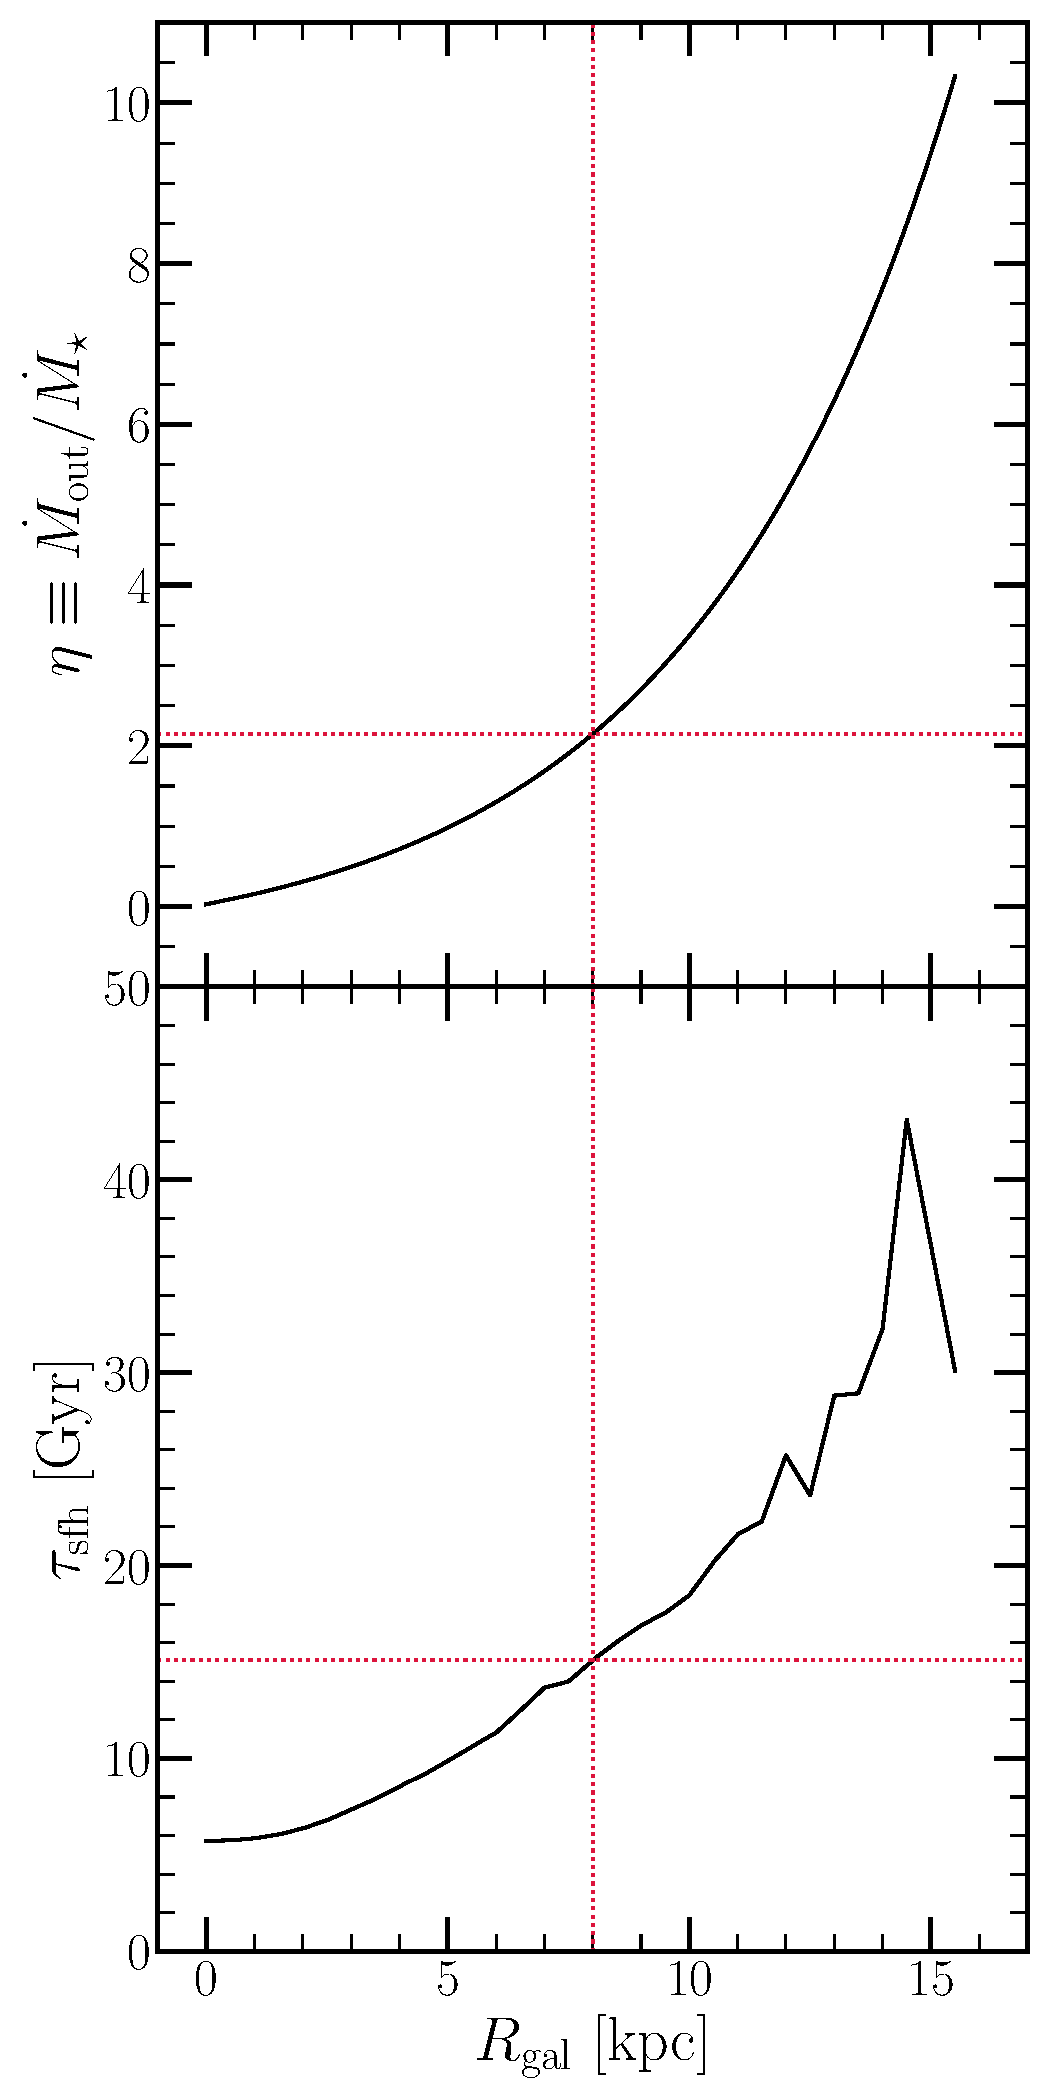
\includegraphics[scale = 0.45]{eta_tau_sfh.pdf} 
\caption{\textbf{Top}: Our implemented scaling of the mass loading factor 
$\eta$~with Galactocentric radius (black) as defined by equation 
\refp{eq:eta_rgal}.~\textbf{Bottom}: The e-folding timescales of the star 
formation histories of our model galaxies (black). These values come from a 
fit to the~$\Sigma_\star$-age relation in bins of~$R/R_\text{e}$~for 
$10^{10.5}$~-~$10^{11}$~\msun~Sa/Sb Hubble type spiral galaxies as reported by 
\citet[][see discussion in~\S~\ref{sec:methods:sfhs}]{Sanchez2020}. The 
horizontal and vertical red dashed lines in both panels highlight a mass 
loading factor of~$\eta \approx$~2.15 and a star formation timescale of 
$\tau_\text{sfh} \approx$~15 Gyr at an assumed radius of the sun of 
$R_\odot$ = 8 kpc. } 
\label{fig:eta_tau_sfh} 
\end{figure} 

Both AGB star enrichment and the recycling of previously produced metals in 
this paper proceed as they did in~\citet{Johnson2020}, with the caveat that the 
mass is added to the annulus that a stellar population is in at a given time, 
which may or may not be the annulus it was born in. Recycling proceeds 
according to the~\citet{Kalirai2008} initial-remnant mass relation assuming a 
\citet{Kroupa2001} IMF and a mass-lifetime relationship of 
$\tau = 1.1\tau_\odot(M/M_\odot)^{-3.5}$, where~$\tau_\odot$~= 10 Gyr is the 
main sequence lifetime of the sun and the factor of 1.1 accounts for the 
post-main sequence lifetime.~\texttt{VICE} in its current version forces an AGB 
enrichment channel in all models; it is thus included in the present paper. For 
this enrichment channel, we adopt the net yields sampled on a table of stellar 
initial mass and metallicity from the FRUITY database \citep{Cristallo2011}. 
However, the AGB star yields of O and Fe are negligible compared to their 
supernova yields; we therefore conclude discussion of this component of our 
models here. 
\par 

\subsection{Star Formation Histories} 
\label{sec:methods:sfhs} 
\texttt{VICE} handles models in either infall, star formation, or gas mode, 
referring simply to which component of the evolutionary history the user has 
specified. The starburst models presented in~\citet{Johnson2020} ran in infall 
mode, but here we run~\texttt{VICE} in star formation mode, because we are 
after specific forms for the star formation histories of our models. In 
Appendix~\ref{sec:normalize_sfh}, we present justification of how we normalize 
the parameters of our star formation histories to produce a realistic model 
Galaxy at the present day. In short, it takes in a unitless description of the 
dependence of the SFH at a given Galactocentric radius, denoted 
$f(t|R_\text{gal})$, and a unitless description of the present day stellar 
surface density gradient, denoted~$g(R_\text{gal})$. We integrate 
$f(t|R_\text{gal})$ with time for each annulus, assuming~$R_\text{gal}$ to 
correspond to the centre of the zone, and attach a prefactor to 
$f(t|R_\text{gal})$ in each annulus such that the desired gradient is achieved 
with a total stellar mass similar to the Milky Way. This procedure neglects the 
impact of radial migration, assuming that it does not significantly alter the 
form of~$g(R_\text{gal})$. We demonstrate that these assumptions hold in~\S 
\ref{sec:methods:surface_density_gradient}, in which we also detail our 
adopted form of~$g(R_\text{gal})$. As long as this assumption is not violated, 
the equation derived in Appendix~\ref{sec:normalize_sfh} can be used to 
calculate these prefactors for future models of Milky Way-like galaxies. 
\par 
In the present paper, we present four fiducial SFHs, which we dub ``constant'', 
``inside-out'', ``late-burst'', and ``outer-burst''. They're defined as 
follows: 
\begin{itemize} 
	\item \textbf{Constant}: The SFH at a given radius is time-independent. 
	\begin{equation} 
	f_\text{C}(t|R_\text{gal}) = 1 
	\label{eq:constant_sfh} 
	\end{equation} 
	This case is of particular theoretical interest because it quantifies the 
	effect of stellar migration while removing the impact of a time-dependent 
	SFH. 

	\item \textbf{Inside-Out}: This is our fiducial SFH. 
	\begin{equation} 
	f_\text{IO}(t|R_\text{gal}) = (1 - e^{-t / \tau_\text{rise}}) 
	e^{-t / \tau_\text{sfh}} 
	\label{eq:insideout_sfh} 
	\end{equation} 
	We adopt this mathematical form over a more traditional 
	linear-times-exponential characterization, because the latter does not 
	offer control over the position of the maximum SFR. The form we adopt has 
	a maximum near~$\tau_\text{rise}$, for which we adopt a value of 2 Gyr 
	everywhere here. This produces a peak in star formation at lookback times 
	of~$\sim$10 Gyr, roughly corresponding to a redshift of~$z \approx$~2, in 
	agreement with observational results on the cosmic SFH~\citep{Madau2014}. 
	In this paper,~$\tau_\text{sfh}$ is a function of~$R_\text{gal}$, discussed 
	in this section. We present results assuming this model throughout this 
	paper except in cases where a different SFH impacts the predictions. 

	\item \textbf{Late-Burst}: In this model, the inside-out SFH is modified to 
	exhibit a recent, gradual burst in star formation described by a Gaussian: 
	\begin{equation} 
	f_\text{LB}(t|R_\text{gal}) = f_\text{IO}(r|R_\text{gal}) 
	(1 + A_be^{-(t - t_b)^2/2\sigma_b^2}) 
	\label{eq:lateburst_sfh} 
	\end{equation} 
	$A_b$ is a dimensionless parameter describing the strength of the 
	starburst,~$t_b$ is the time of the local maximum in the SFH during the 
	burst, and~$\sigma_b$ is the width of the Gaussian describing it. This 
	model being loosely motivated by the findings of~\citet{Mor2019} and 
	\citet{Isern2019}, we adopt~$A_b$ = 1.5,~$t_b$ = 10.2 Gyr, and 
	$\sigma_b$ = 1 Gyr, finding in practice that~$A_b$ = 1.5 produces a 
	local maximum SFR that is a factor of~$\sim$2 larger than the preceding 
	local minimum. 

	\item \textbf{Outer-Burst}: A variation of the late-burst model in which 
	only~$R_\text{gal} \geq$~6 kpc experience the starburst. This is loosely 
	motivated by the findings of~\citet{Vincenzo2020} where a hydrodynamical 
	simulation of a Milky Way-like galaxy showed radially dependent infall. 
	\begin{equation} 
	f_\text{OB}(t|R_\text{gal}) = \begin{cases} 
	f_\text{IO}(t|R_\text{gal}) & (R_\text{gal} < 6\text{ kpc}) \\ 
	f_\text{LB}(t|R_\text{gal}) & (R_\text{gal} \geq 6\text{ kpc}) 
	\end{cases} 
	\label{eq:outerburst_sfh} 
	\end{equation} 
\end{itemize} 
Although we do not consider such models here, an investigation into the impact 
of more episodic star formation histories would be an interesting extension of 
the present paper. For example,~\texttt{VICE} has all of the necessary 
capabilities to handle models in which major episodes of star formation 
coincide with close passages of the Sagittarius dwarf 
\citep[e.g.][]{RuizLara2020}. 
\par 
We derive the scaling of the e-folding timescales of star formation 
$\tau_\text{sfh}$ with~$R_\text{gal}$ from the data in~\citet{Sanchez2020}. 
They present the stellar surface density~$\Sigma_\star$ as a function of age 
in bins of~$R/R_\text{e}$ for MaNGA galaxies, where~$R_\text{e}$ is the 
half-light radius. Here we take their~$M_\star = 10^{10.5} - 10^{11}$ 
\msun~ bin for Sa/Sb spirals and simultaneously fit the normalization and 
e-folding timescale~$\tau_\text{sfh}$ of our~$f_\text{IO}(t|R_\text{gal})$ form 
to the data. Although the normalization is irrelevant to our models and 
determined via the method outlined in Appendix~\ref{sec:normalize_sfh}, we 
adopt the resulting~$\tau_\text{sfh}-R_\text{gal}$ relation in our models. With 
our adopted stellar surface density gradient (see discussion in~\S 
\ref{sec:methods:surface_density_gradient}), we know the present-day half-mass 
radius to be very near 4 kpc. The findings of~\citet{Garcia-Benito2017} and 
\citet{GonzalezDelgado2014} suggest that half-light radii are marginally larger 
than half-mass radii. Based on equation (4) of~\citet{GonzalezDelgado2014} 
relating the two for circular apertures, we expect our model Galaxy to have a 
half-light radius near 5 kpc. We therefore adopt~$R_\text{e}$ = 5 kpc to 
convert the~$\tau_\text{sfh}-R_\text{gal}/R_\text{e}$ relation resulting from 
our fit to the~\citet{Sanchez2020} data into a~$\tau_\text{sfh}-R_\text{gal}$ 
relation. {\color{red} If there are references suggesting a similar value for 
the Milky Way, we should note them here. } 
\par 
We illustrate this relationship in the bottom panel of Fig. 
\ref{fig:eta_tau_sfh}, noting that the resulting timescales are long, 
particularly for the outer Galaxy. With a red dotted line, we highlight a value 
of~$\tau_\text{sfh} \approx$~15 Gyr at an assumed orbital radius of the sun of 
$R_\odot$ = 8 kpc. Although these timescales at most radii are considerably 
longer than a Hubble time, this is no cause for worry; this simply means that 
these regions of the Galaxy in our models experience less than 1 e-folding in 
their SFR, and that in the outer Galaxy the SFH is nearly constant after the 
initial rise in the first~$\sim$2 Gyr. It is nonetheless interesting that 
these timescales are considerably longer than that derived for the cosmic 
SFH~\citep{Madau2014}. 

% fig 4 
\begin{figure*} 
\centering 
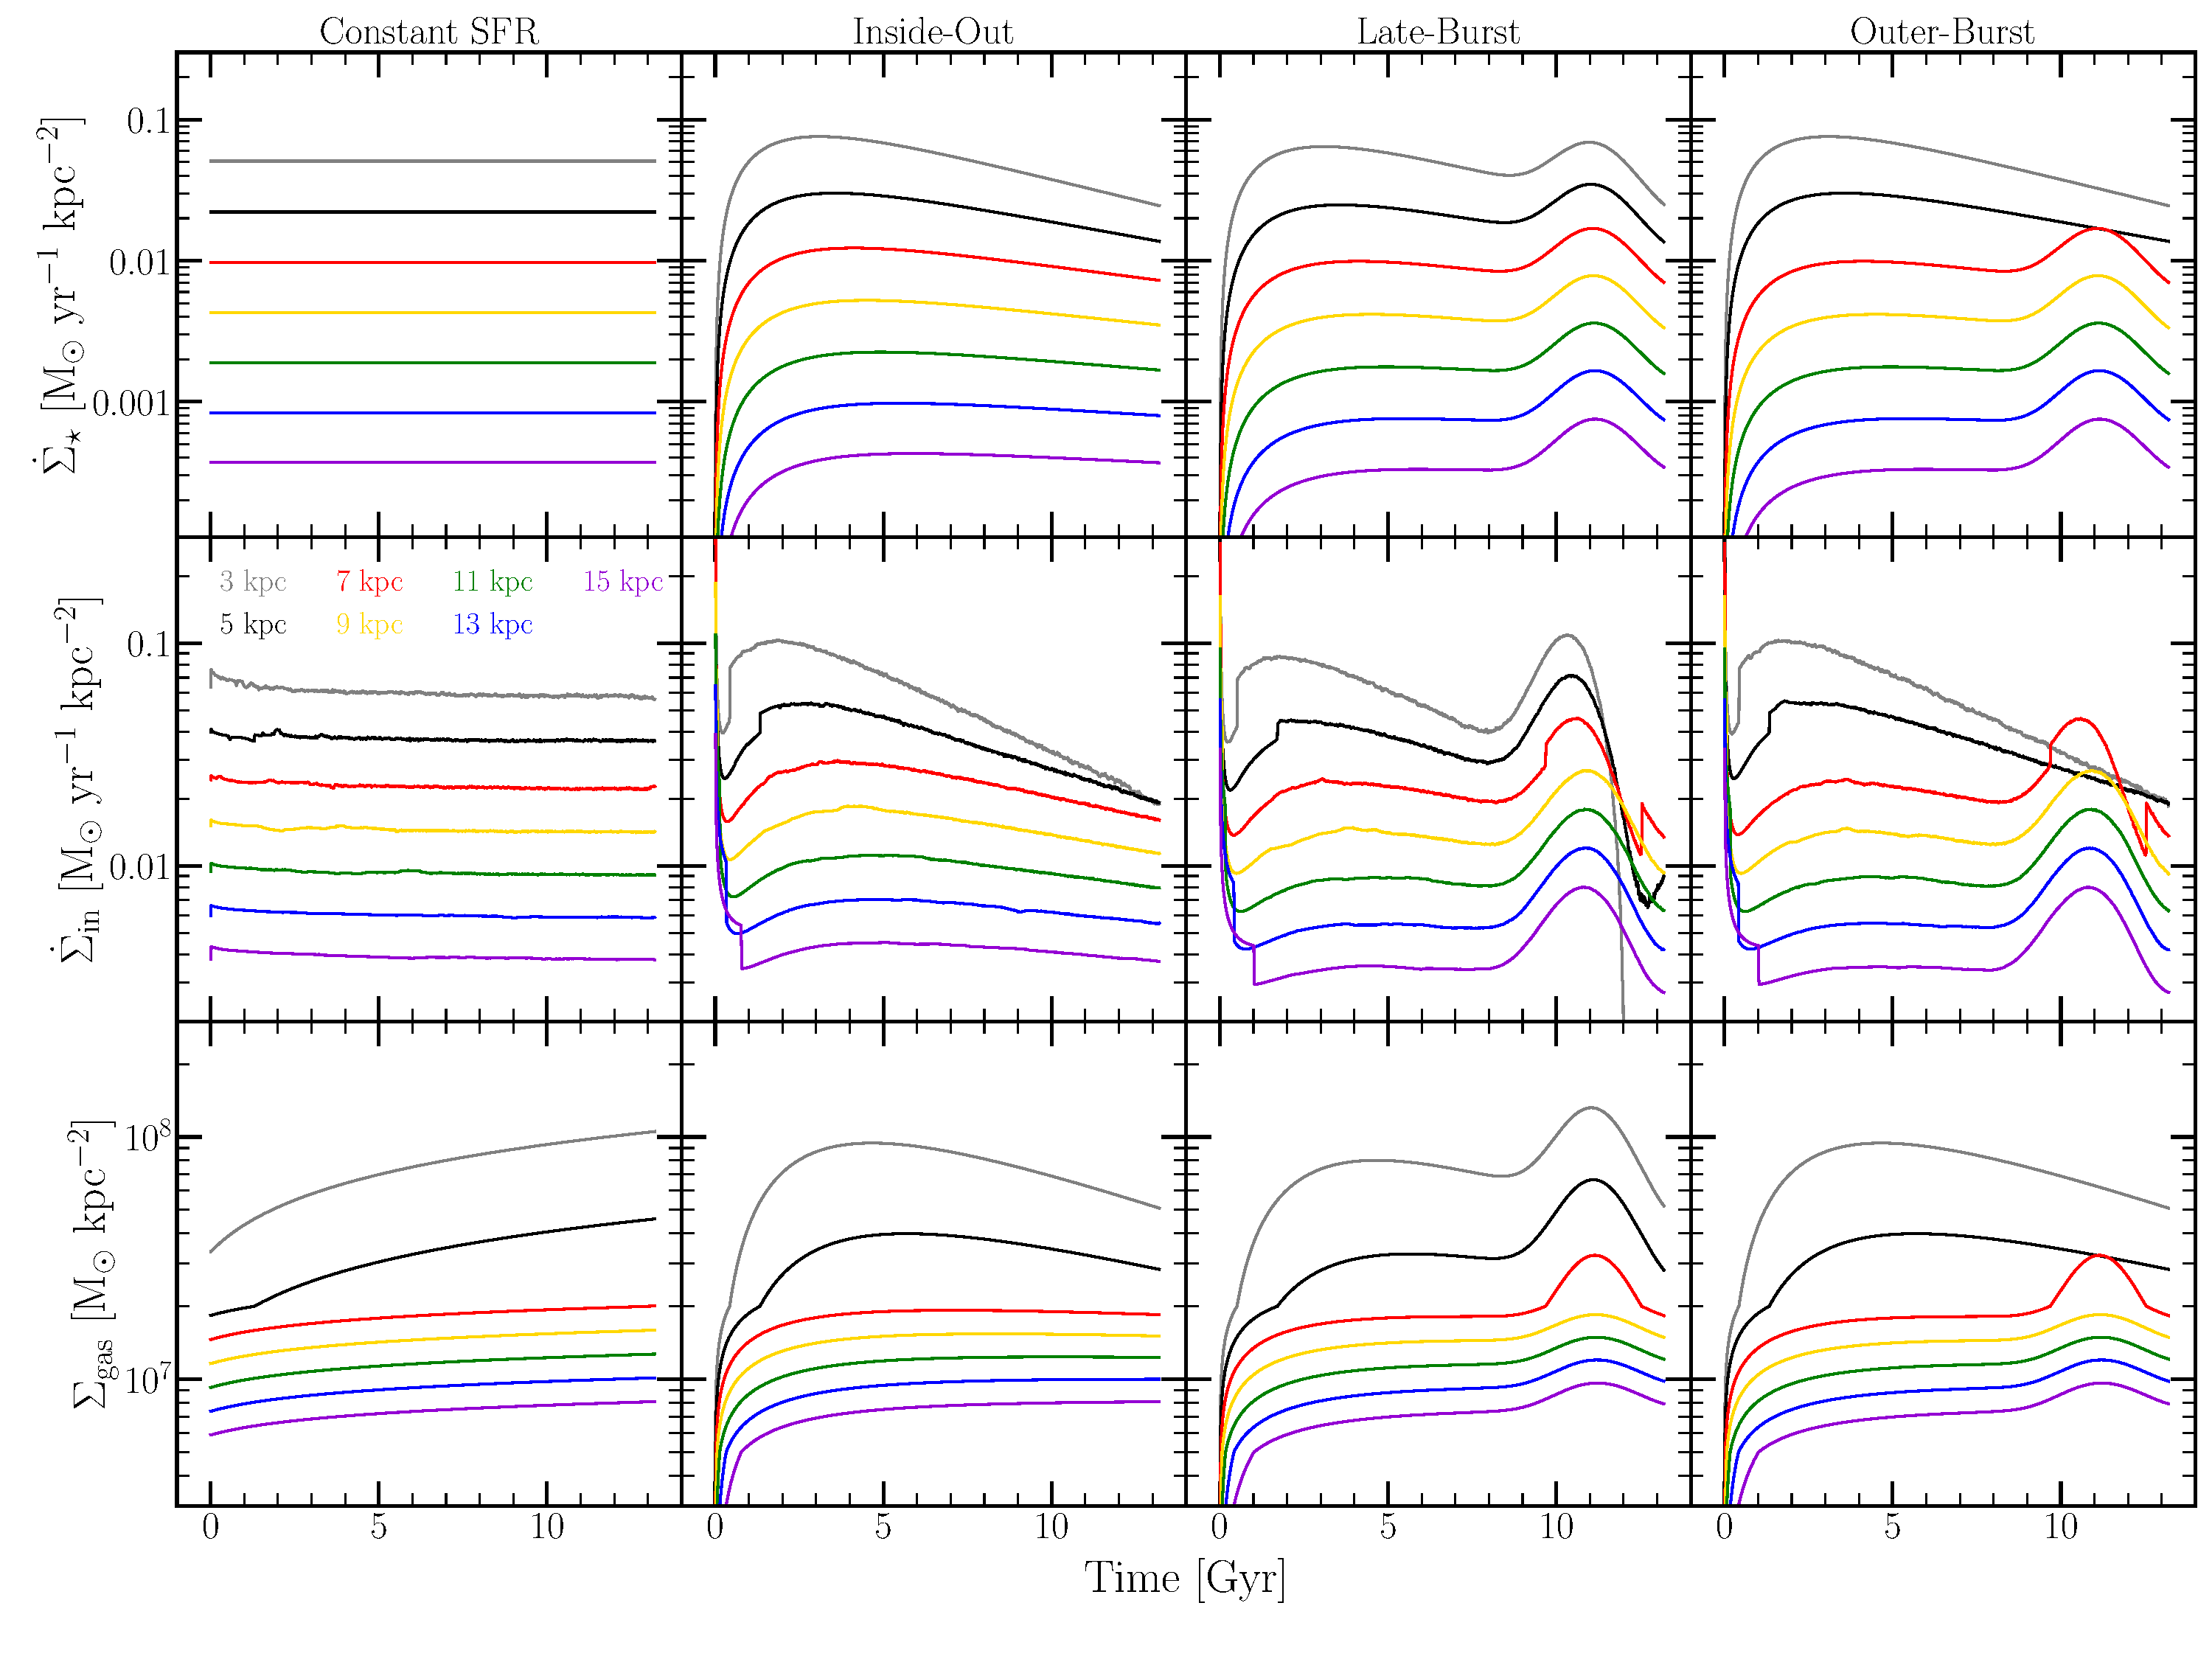
\includegraphics[scale = 0.32]{evol.pdf} 
\caption{The surface densities of star formation~$\dot{\Sigma}_\star$ (top 
row), infall $\dot{\Sigma}_\text{in}$ (middle row), and gas~$\Sigma_\text{g}$ 
(bottom row) as functions of simulation time for our four fiducial SFHs: 
constant (far left), inside-out (left middle), late-burst (right middle), and 
outer-burst (far right). We plot curves for the annuli whose inner radii are 
3 kpc (grey), 5 kpc (black), 7 kpc (red), 9 kpc (yellow), 11 kpc (green), 13 
kpc (blue), and 15 kpc (purple) (see equations~\refp{eq:constant_sfh}, 
\refp{eq:insideout_sfh},~\refp{eq:lateburst_sfh}, and~\refp{eq:outerburst_sfh} 
for the mathematical definition of each SFH). 
}
\label{fig:evol} 
\end{figure*} 

We plot the resultant SFHs or our models in the top row of Fig.~\ref{fig:evol} 
for a handful of radii. At all timesteps, the gas supply is known via the star 
formation efficiency timescale~$\tau_\star$ (see discussion in~\S 
\ref{sec:methods:sfe}). This quantity is illustrated in the bottom row of 
Fig.~\ref{fig:evol}.~\texttt{VICE} automatically calculates the implied infall 
rate by comparing the amount of gas lost to outflows and star formation in a 
given timestep to that which is required to sustain the user-specified level of 
star formation at the next timestep; we assume the infalling gas to be of zero 
metallicity at all times. This quantity is shown in the middle row of Fig. 
\ref{fig:evol}. 

\subsection{Star Formation Efficiency} 
\label{sec:methods:sfe} 
The term ``star formation efficiency'' (SFE) is somewhat overloaded in the 
literature. In the star formation and feedback community, it usually 
refers to the fraction of a molecular cloud's mass which will eventually be 
converted into stars. In the chemical evolution literature, however, it 
typically refers to the inverse timescale relating the SFR within some star 
forming reservoir and the mass of gas in that region: 
$\tau_\star \equiv \Sigma_\text{g}/\dot{\Sigma}_\star$. High (Low) values of 
$\tau_\star$ indicate slow (fast) star formation and thus low (high) SFE; when 
we refer to SFE here, we're referring to the definition based on this 
timescale. In the star formation and feedback literature, this is often 
referred to as the ``depletion time''. 
\par 
Based on the findings of~\citet{Kennicutt1998}, it is common practice in the 
chemical evolution literature a single power-law describing the relationship 
between the surface densities of gas and star formation~$\Sigma_\text{g}$ and 
$\dot{\Sigma}_\star$, often referred to as the star formation law or the 
Kennicutt-Schmidt relation: 
\begin{equation} 
\dot{\Sigma}_\star \sim \Sigma_\text{g}^N 
\end{equation} 
\citet{Kennicutt1998} derive~$N = 1.4 \pm 0.15$ relating the total 
$\dot{\Sigma}_\star$~and~$\Sigma_\text{g}$~within the disc across a sample of 
quiescent spiral galaxies and infrared and circumnuclear starbursts. However, 
recent studies have found evidence that much of the observed scatter in this 
relation is physical in origin~\citep{delosReyes2019} and that there are 
significant breaks in both the power-law index and zero-points 
\citep{Kennicutt2020}. Much of the uncertainty surrounding the details of the 
star formation law is a consequence of the ongoing debate about the CO-to-H$_2$ 
conversion factor (\citealp{Kennicutt2012};~\citealp*{Liu2015}). Although 
\citet{Ellison2020a} demonstrate that there are significant galaxy-to-galaxy 
variations in the star formation law, suggesting that individual galaxies do 
not follow the population averaged trend,~\citet{delosReyes2019} argue that 
this is still a reasonable recipe for Galaxy evolution models. We adopt such a 
formalism here. 
\par 
\citet{Krumholz2018} compare model-predicted star formation laws to the 
observations of~\citet{Bigiel2010} and~\citet{Leroy2013} (see their Fig. 2). We 
find that the following by-eye fit to the power-law index~$N$~is a reasonble 
description of the aggregate data: 
\begin{equation} 
N = \begin{cases} 
1.0 & (\Sigma_\text{g} \geq \Sigma_{\text{g},2}) \\ 
3.6 & (\Sigma_{\text{g},1} \leq \Sigma_\text{g} \leq \Sigma_{\text{g},2}) \\ 
1.7 & (\Sigma_\text{g} \leq \Sigma_{\text{g},1}) 
\end{cases} 
\label{eq:sf_law_indeces} 
\end{equation} 
where~$\Sigma_{\text{g},1} = 5\times10^6$~\msun~\persqkpc~and 
$\Sigma_{\text{g},2} = 2\times10^7$~\msun~\persqkpc. The apparent linearity of 
the relationship above~$\sim2\times10^7$~\msun~\persqkpc~suggests that in this 
regime, star formation proceeds at the fastest possible rate, and that 
$\tau_\star \equiv \Sigma_\text{g}/\dot{\Sigma}_\star$~= constant. The 
observations of~\citet{Leroy2013} and~\citet{Kennicutt2020} would suggest that 
these are the 
surface densities at which the molecular fraction~$f_\text{mol} = M_{\text{H}_2} 
/ (M_{\text{H}_2} + M_\text{HI}) \approx$~1. We therefore adopt the assumption 
that above~$\Sigma_\text{g} = 2\times10^7$~\msun~\persqkpc,~$\tau_\star$ 
reaches its minimum value, and increases with decreasing~$f_\text{mol}$. We 
denote this value as~$\tau_\text{mol}$, the value of~$\tau_\star$ for a gas 
reservoir with~$f_\text{mol}$~= 1. This, combined with our three-component 
power-law index N results in the following final form for our adopted star 
formation law: 
\begin{equation} 
\dot{\Sigma}_\star = \begin{cases} 
\Sigma_\text{g} \tau_\text{mol}^{-1} & 
(\Sigma_\text{g} \geq \Sigma_{\text{g},2}) 
\\ 
\Sigma_\text{g} \tau_\text{mol}^{-1} \left(\frac{
	\Sigma_\text{g}
}{
	\Sigma_{\text{g},2} 
}\right)^{2.6} & 
(\Sigma_{\text{g},1} \leq \Sigma_\text{g} \leq \Sigma_{\text{g},2}) 
\\ 
\Sigma_\text{g} \tau_\text{mol}^{-1} \left(\frac{
	\Sigma_{\text{g},1} 
}{
	\Sigma{\text{g},2} 
}\right)^{2.6}\left(\frac{
	\Sigma_\text{g}
}{
	\Sigma_{\text{g},1} 
}\right)^{0.7} & 
(\Sigma_\text{g} \leq \Sigma_{\text{g},1}) 
\end{cases} 
\label{eq:sf_law} 
\end{equation} 
where we choose the power-law indeces such that this formalism is consistent 
with equation~\refp{eq:sf_law_indeces}, and prefactors are added to ensure 
piece-wise continuity. In implementation,~\texttt{VICE} requires the 
$\tau_\star-\dot{\Sigma}_\star$ relation when ran in star formation mode and 
the~$\tau_\star-\Sigma_\text{g}$ relation when ran in infall and gas modes. 
Both follow algebraically from this relationship given the substitution 
$\tau_\star \equiv \Sigma_\text{g} / \dot{\Sigma}_\star$. 
\par 
Although it is more physically motivated to use an adopted star formation law 
to infer a star formation rate from the ISM properties at a given timestep, as 
discussed in~\S~\ref{sec:methods:sfhs}, we are using~\texttt{VICE} in star 
formation mode. This means that it is~$\dot{\Sigma}_\star$ which is specified 
\textit{a priori} by our models - not~$\Sigma_\text{g}$. That is,~\texttt{VICE} 
is inferring~$\Sigma_\text{g}$ from~$\dot{\Sigma}_\star$ in our models, not 
the other way around. While we acknowledge the findings of~\citet{Ellison2020b}, 
this another reason we must invoke a simple parameterization for the star 
formation law, which~\citet{Kennicutt2020} argue is still a reasonable 
approach. This decision also means that changing our assumptions about the 
star formation law do not impact our SFHs, instead impacting the inferred 
$\Sigma_\text{g}$ as a function of radius and time. 
\par 
Based on the observed Kennicutt-Schmidt at different redshifts, 
\citet{Tacconi2018} suggest that~$\tau_\text{mol}$ should scale with redshift 
$z$ and the deviation from the star forming main sequence~$\delta$MS via 
$\tau_\text{mol} \propto (1 + z)^{-0.6}\delta\text{MS}^-0.44$. We don't take 
into account the effect of~$\delta$MS in our models, but we do investigate the 
redshift dependence. A reasonable approximation to the~$t - z$ relation out to 
$z \approx$~3 assuming typical~$\Lambda$CDM cosmology is given by: 
\begin{equation} 
\frac{t}{t_0} \approx (1 + z)^{-5/4} 
\end{equation} 
where~$t_0$ is the present-day age of the universe, and~$t$ is not simulation 
time but the age of the universe. Plugging this relation into the 
\citet{Tacconi2018} scaling yields the following time-dependence for 
$\tau_\text{mol}$: 
\begin{equation} 
\tau_\text{mol} = \tau_{\text{mol},0}(t/t_0)^{12/25} \approx 
\tau_{\text{mol},0}(t/t_0)^{1/2} 
\end{equation} 
where~$\tau_{\text{mol},0}$ is simply~$\tau_\text{mol}$ at the present day. We 
generalize this formula to the following form: 
\begin{equation} 
\tau_\text{mol} = \tau_{\text{mol},0}(t/t_0)^\gamma 
\label{eq:tau_mol}
\end{equation} 
In this paper we present models which adopt~$\tau_{\text{mol},0}$ = 2 Gyr 
\citep{Leroy2008, Leroy2013, Tacconi2018} and~$\gamma$ = 1/2 based on this 
argument. We have also ran simulations which adopt~$\tau_{\text{mol},0}$ = 1 
Gyr and~$\gamma$ = 0 (a time-independent~$\tau_\text{mol}$), and found similar
results. In all timesteps an annnuli,~\texttt{VICE} infers~$\Sigma_\text{g}$ 
from~$\dot{\Sigma}_\star$ given our equations~\refp{eq:sf_law} and 
\refp{eq:tau_mol}. 

% fig 5 
\begin{figure} 
\centering 
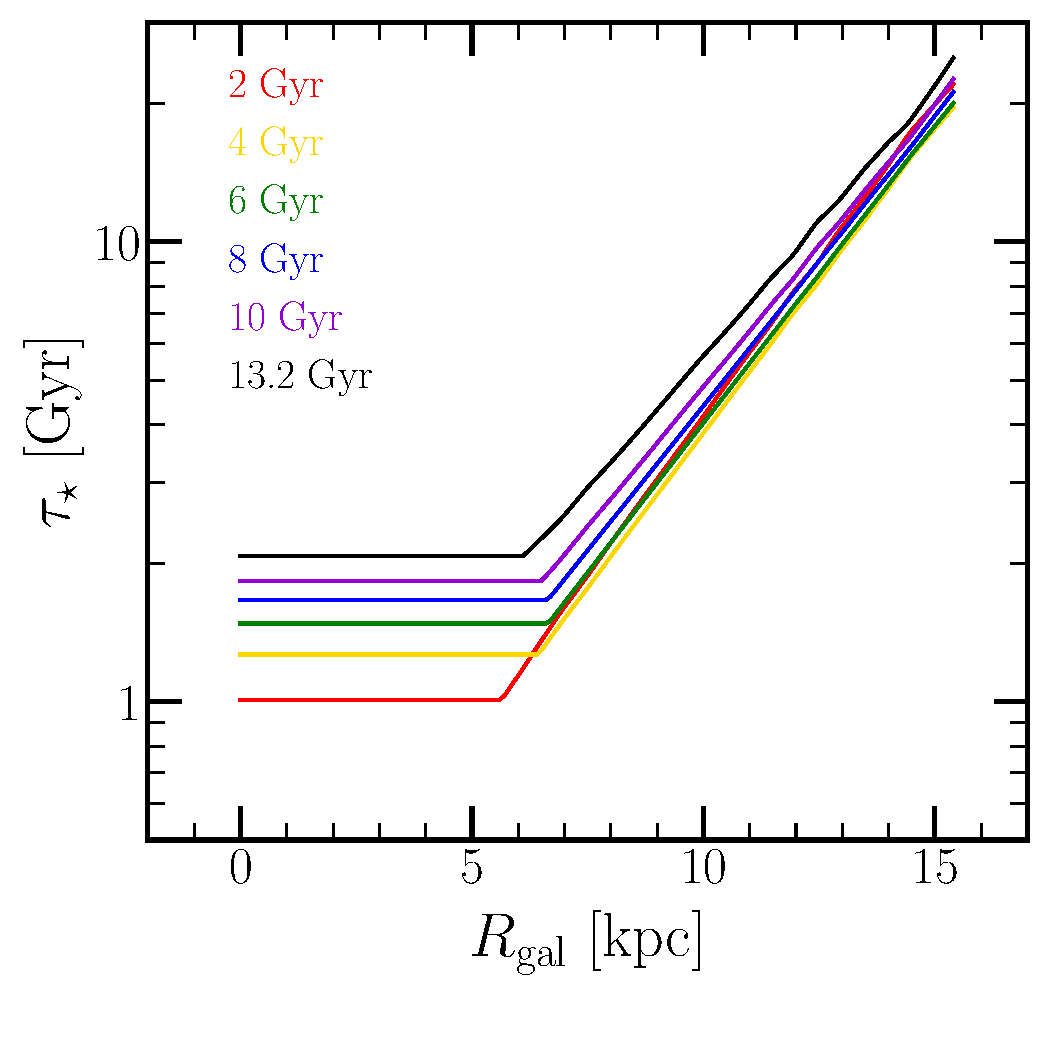
\includegraphics[scale = 0.45]{sfe.pdf} 
\caption{The star formation efficiency timescale~$\tau_\star$ as a function of 
Galactocentric radius at simulation times of 2 Gyr (red), 4 Gyr (yellow), 
6 Gyr (green), 8 Gyr (blue), 10 Gyr (purple), and 12.2 Gyr (the present day, 
black) predicted by our inside-out SFH model. } 
\label{fig:sfe} 
\end{figure} 

In Fig.~\ref{fig:sfe}, we plot~$\tau_\star$ as a function of~$R_\text{gal}$ at 
six different time stamps predicted by our fiducial, inside-out SFH model. At 
$R_\text{gal} \lesssim$ 6 kpc,~$\tau_\star$ is near~$\tau_\text{mol}$ at all 
times, implying a molecular fraction of unity at these radii. Although this 
prediction is likely unrealistic because 21-cm line observations suggest the 
presence of neutral hydrogen as close to the Galactic centre as several hundred 
pc~\citep{Kalberla2009}, we find in practice that changing our assumptions 
about the star formation law does not impact our conclusions. In collecting 
results for this paper, we investigated purely linear, purely power-law, and 
broken power-law characterizations, finding similar predictions in all cases. 
In general we find that the detailed form of the SFH, and to some extent the 
time-dependence of radial migration, exert much greater power in establishing 
the model predictions than does the star formation law. Nonetheless it is an 
interesting result that a~$\dot{\Sigma}_\star - \Sigma_\text{g}$ relation 
informed by the observed, population averaged trend and the normalization of 
our SFHs implied by the stellar mass of the Milky Way predicts such a 
discrepancy with the observed HI distribution. We refrain from further 
discussion of this with the finding that it doesn't impact the conclusions 
detailed in the present paper. 

\subsection{Surface Density Gradient} 
\label{sec:methods:surface_density_gradient} 

% fig 6 
\begin{figure} 
\centering 
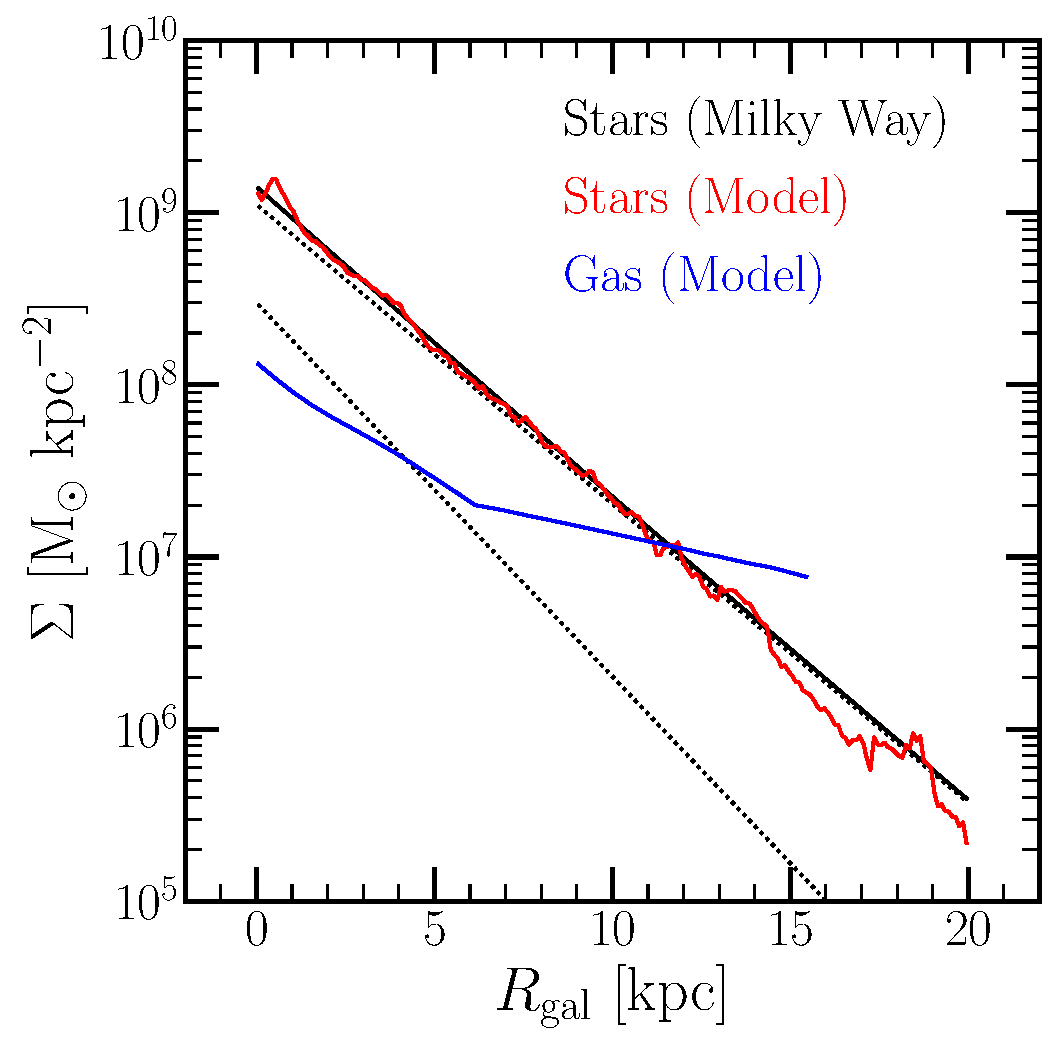
\includegraphics[scale = 0.45]{surface_density_gradient.pdf} 
\caption{The surface density of gas (blue) and stars (red) as predicted by our 
inside-out SFH model. The dotted black line with the higher normalization 
denotes a thin disc profile with scale length~$R_t$ = 2.5 kpc; the other 
denotes a thick disc profile with scale length~$R_T$ = 2.0 kpc, and a ratio of 
$\Sigma_T/\Sigma_t$~= 0.27 at~$R_\text{gal}$~= 0. The solid black line denotes 
the sum of the two; this is the surface density gradient of the Milky Way as 
reported by~\citet{Bland-Hawthorn2016}, renormalized to imply the same total 
stellar mass within the disc as our models. } 
\label{fig:surface_density} 
\end{figure} 

As discussed in~\S~\ref{sec:methods:sfhs}, Appendix~\ref{sec:normalize_sfh} 
presents justification of a recipe in which we select a unitless function 
describing the stellar surface density gradient~$g(R_\text{gal})$. In setting 
the normalization, our model ensures that the integral of~$g(R_\text{gal})$ 
over the surface area of the disc predicts a total stellar mass in agreement 
with that observed for the Milky Way. For this value, we adopt 
$M_\star^\text{MW} = (6.08 \pm 1.14)\times10^{10}$~\msun~\citep{Licquia2015}. 
This is the total stellar mass of the Galaxy, including the bulge; 
\citet{Licquia2015} report~$(5.17 \pm 1.11)\times10^{10}$~\msun~as the mass of 
the disc alone. Although we aren't modeling the bulge here, our model extends 
to~$R_\text{gal}$ = 0 and our sample of candidate analog star particles from 
\texttt{h277} includes those with bulge-like kinematics. 
\par 
In this paper we adopt the following double exponential form for 
$g(R_\text{gal})$, describing the thin and thick disc components of the 
Galaxy: 
\begin{equation} 
g(R_\text{gal}) = e^{-R_\text{gal}/R_t} + \frac{\Sigma_T}{\Sigma_t} 
e^{-R_\text{gal}/R_T} 
\label{eq:gradient} 
\end{equation} 
where~$R_t$~and~$R_T$~are the scale radii of the thin and thick discs, 
respectively, and~$\Sigma_T/\Sigma_t$~is the ratio of their surface densities 
at~$R_\text{gal}$~= 0. We adopt~$R_t$~= 2.5 kpc,~$R_T$~= 2.0 kpc, and 
$\Sigma_T/\Sigma_t$~= 0.27 based on the findings of~\citet{Bland-Hawthorn2016}. 
We plot the single exponential forms of each disc component as a dotted black 
line in Fig.~\ref{fig:surface_density}, with the solid black line denoting the 
sum of the two. Althoug these scale radii are smaller than the commonly adopted 
scale radius for a single exponential disc of~$r_s \approx$~3 kpc 
\citep[e.g.][]{Binney2008}, our choice of a double exponential disc here 
necessitates a choice be made for not one but two scale radii. 
\par 
We plot the resultant surface density gradients from our fiducial, inside-out 
SFH model in Fig.~\ref{fig:surface_density} as well, with red denoting the 
stellar gradient and the gas in blue. We note that the stellar gradient very 
nearly follows our target gradient denoted by the solid black line and 
expressed by equation~\refp{eq:gradient}. Stellar migration has indeed not 
altered the overall form of the gradient, simply introducing scatter around the 
adopted trend. Although there are slight enhancements at small~$R_\text{gal}$ 
and deficits at large~$R_\text{gal}$, the agreement is excellent in the regions 
of the Galaxy where the gradient is best constrained observationally. The 
$R_\text{gal}$ > 15.5 kpc populations are also composed entirely of stars that 
migrated there, since that is the radius at which we shut of star formation; 
with this mind, the under-prediction at these radii is unsurprising. 
Furthermore, in this paper we are interested primarily in the~$R_\text{gal}$~= 
3 - 15 kpc range anyway, since this is the region where disc stars are the 
dominant populations. We also note that the gas gradient
shows a break in the scale radius near~$R_\text{gal} \approx$ 
6 kpc. This is a consequence of our adopted star formation law; at 
$\Sigma_\text{g} = 2\times10^7$~\msun~\persqkpc~the relation changes from 
linear at higher densities to~$\dot{\Sigma}_\star \sim \Sigma_\text{g}^{3.6}$ 
at lower densities (see discussion in~\S~\ref{sec:methods:sfe}). Because we are 
running~\texttt{VICE} in star formation mode, it's more accurate to say that 
$\Sigma_\text{g}$~is a weak function of~$\dot{\Sigma}_\star$~at 
$\Sigma_\text{g} \leq 2\times10^7$~\msun~\persqkpc~in this range as opposed to 
$\dot{\Sigma}_\star$~being a strong function of~$\Sigma_\text{g}$. When looking 
at the present-day gradient, this presents as a flattening of the gradient at 
the radius where~$\Sigma_\text{g} = 2\times10^7$~\msun~\persqkpc; further 
inspection along the y-axis of Fig.~\ref{fig:surface_density} confirms that 
this break indeed occurs at this value of~$\Sigma_\text{g}$. 
\par 
Although we adopt the~\citet{Licquia2015} stellar mass of the Milky Way here, 
we find similar results when taking a value which differs by an order of 
magnitude. While mass typically cancels in one-zone models of chemical 
evolution, the abundances instead determined by the evolutionary parameters 
(e.g.~$\eta$~and~$\tau_\star$), this value sets the normalization of the 
SFH~$\dot{\Sigma}_\star(t, R_\text{gal})$ in our models. In turn this impacts 
the surface densities of gas~$\Sigma_\text{g}$ inferred at each timestep, and 
thus the abundances to some extent. This choice only matters insofar as the 
choice of star formation law matters, which we find to not impact our 
conclusions. 

\subsection{Summary} 
\label{sec:methods:summary} 
In summary, our fiducial model has an inside-out SFH with e-folding timescales 
derived from the observations of~\citet[][see discussion in~\S 
\ref{sec:methods:sfhs}]{Sanchez2020}. Radial migration proceeds in a manner in 
which our model stellar populations have a change in radius 
$\Delta R_\text{gal}$ informed from the~\texttt{h277} hydrodynamical simulation 
\citep[][see discussion in~\S~\ref{sec:methods:h277}]{Christensen2012, 
Zolotov2012, Loebman2012, Loebman2014, Brooks2014}. In the base-line model, 
stars move to their final radius with a~$\sqrt{\text{age}}$~dependence 
(\citealp{Frankel2018, Frankel2020} model stellar migration with a similar 
characterization; see discussion in~\S~\ref{sec:methods:migration}). Using 
\texttt{VICE} to calculate abundances for O and Fe in this paper, our supernova 
yields are adopted from~\citet{Johnson2020}, who in turn take these values from 
\citet{Weinberg2017}. Outflows are characterized such that the equilibrium 
abundance of oxygen under a constant SFH follows an abundance gradient in 
agreement with observational results in the Milky Way (see discussion in 
\S~\ref{sec:methods:yields};~\citet{Nidever2014} make use of similar 
methodology). Our star formation law is based on the~\citet{Bigiel2010} and 
\citet{Leroy2013} data presented in comparison with theoretical models in 
\citet[][see discussion in~\S~\ref{sec:methods:sfe}]{Krumholz2018}. To describe 
the stellar surface density gradient, we adopt the two-exponential form 
describing the thin and thick discs from~\citet[][see discussion in~\S 
\ref{sec:methods:surface_density_gradient}]{Bland-Hawthorn2016}. 
\par 
Our quality cuts imposed on the star particles from~\texttt{h277} yields a 
sample of 3,000,556 candidate analog star particles (see discussion in~\S 
\ref{sec:methods:h277}), only~$\sim$57\% of which have disc-like kinematics 
at the present day. Since we're modeling the thin and thick disc populations 
here,~$\sim$1.71 million is a much better estimate of the number of star 
particles that we can realistically sample from. We take~$\Delta R_\text{gal}$ 
= 100 pc as the width of each annulus from~$R_\text{gal} = 0$~to 20 kpc and a 
timestep size of~$\Delta T$~= 10 Myr from~$T = 0$~to 12.2 Gyr. With the 
resulting 200 zones and 1,221 timesteps, we let~\texttt{VICE} form~$n = 9$ 
stellar populations per annulus per timestep, resulting in 2,197,000 total 
stellar populations with predicted masses and abundances. While this is more 
than the number of disc particles in our sample of candidate analogs, we force 
the star formation rate to zero beyond~$R_\text{gal}$ = 15.5 kpc; while these 
stellar populations exist within~\texttt{VICE} and are a part of the 
computational overhead, they have zero mass and thus do not contribute to the 
chemical evolution in our models. This results in 1,692,306 stellar 
populations with~\textit{non-zero} masses and abundances predicted by 
\texttt{VICE}, reasonably within the limit of what we can sample. These 
simulations run in~$\sim$2.5 hours and take up~$\sim$235 MB of disc space per 
output, including the extra data that we record for each stellar population's 
analog star particle. Lastly, we adopt a~\citet{Kroupa2001} IMF throughout this 
paper. 
\par 
We have ran~\texttt{VICE} for all four of our SFHs, all four migration 
models, and all four variations in~$\tau_\text{mol}$ noted in~\S 
\ref{sec:methods:sfe} - a total of 64 simulations, as well as a variety of 
other test cases. In this paper, we present results wherever the model 
prescriptions are sensitive to the assumptions. However, in general the 
differences can be understood with only the variations in star formation 
history and the qualitative notion that many stars have moved beyond their 
birth radius. \texttt{VICE} calculates abundances for nearly 2 million stellar 
populations per model; to ensure that resolution does not impact our 
conclusions, we have also ran variations with~$n$~= 2 stellar populations per 
zone per timestep, and found similar results in all cases. 

\section{Comparison to Observations} 
\label{sec:obs_comp} 

% fig 7 
\begin{figure*} 
\centering 
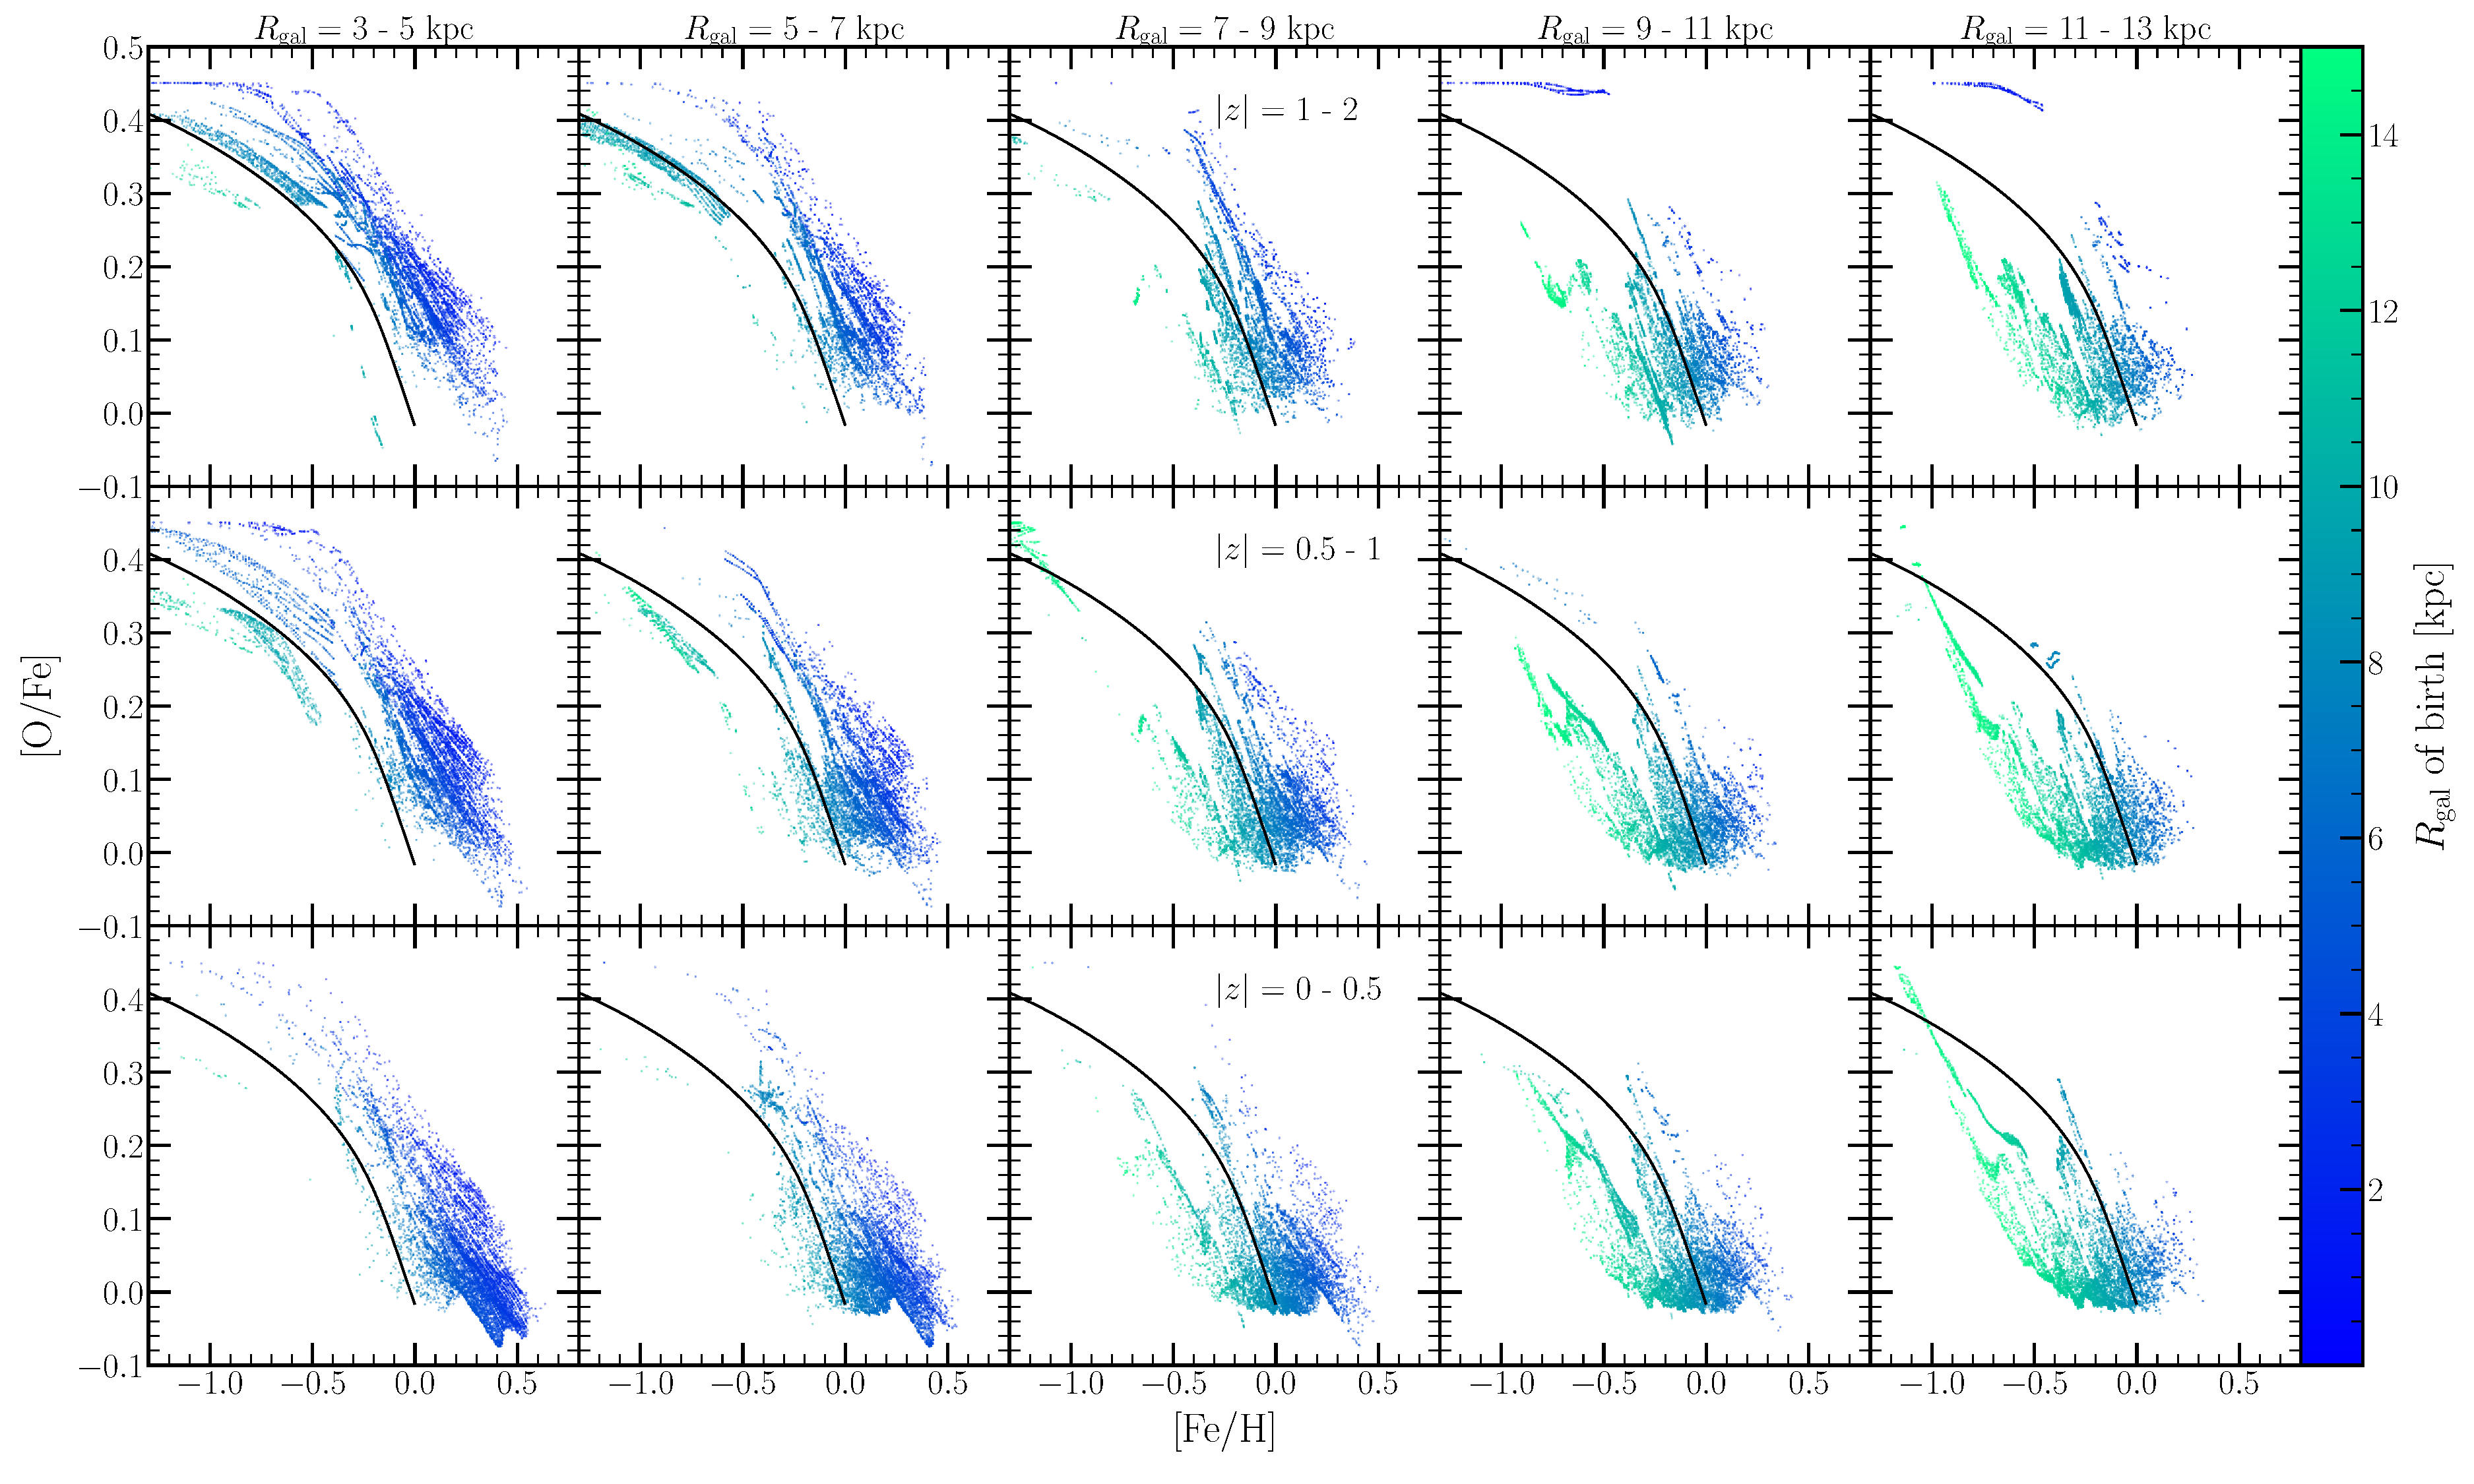
\includegraphics[scale = 0.28]{ofe_feh_densitymap.pdf} 
\caption{[O/Fe]-[Fe/H] diagrams for 15 Galactic regions spanning five bins in 
$R_\text{gal}$ and~$\left|z\right|$. Each region has its own panel, with 
radial bins shown in columns denoted at the top, and with bins in 
$\left|z\right|$ shown in rows denoted in text in the middle column. For each 
region, we plot~$N$~= 10,000 points sampled from our simulated stellar 
populations predicted by our inside-out SFH model, where the probability of 
sampling is proportional to the present-day mass of each stellar population. 
In all panels, points are colour-coded according to the Galactocentric radius 
of birth of the stellar population. For reference, we plot in a solid black 
line in all panels the gas-phase [O/Fe]-[Fe/H] track predicted by the same 
SFH in the~$R_\text{gal}$ = 8 kpc annulus, but with the post-processing 
migration model; this curve is the same in all panels. } 
\label{fig:ofe_feh_diagram} 
\end{figure*} 

We begin the comparison of our model predictions to observational data with the 
distribution of stellar populations in the [O/Fe]-[Fe/H] plane. We separate 
stars into bins based on their present-day Galactic regions defined by five 
bins in~$R_\text{gal}$ (3 - 5, 5 - 7. 7 - 9, 9 - 11, and 11 - 13 kpc) and three 
bins in~$\left|z\right|$ (0 - 0.5, 0.5 - 1, and 1 - 2 kpc). Within each of the 
resulting 15 regions, we sample 10,000 stars at random from our base-line 
inside-out SFH model. Since stars in~\texttt{VICE} are stand-ins for entire 
stellar populations, we let the probability of sampling one of them be 
proportional to its present day mass. We plot the results of this procedure in 
Fig.~\ref{fig:ofe_feh_diagram}, colour-coding each stellar population by its 
birth radius; for reference, we also plot the gas-phase track which resulted 
from the~$R_\text{gal}$ = 8 kpc annulus with the post-processing migration 
model in a black solid line in all panels. 
\par 
In Fig.~\ref{fig:ofe_feh_diagram}, we note that high-$\alpha$~sequence stars 
are predicted to be the dominant population at small~$R_\text{gal}$ and high 
$\left|z\right|$; conversely, the low-$\alpha$~sequence dominates the 
statistics at large~$R_\text{gal}$~and low~$\left|z\right|$. This is consistent 
with the observational results of~\citet{Hayden2015}, who present a density map 
in the [O/Fe]-[Fe/H] for the same Galactic regions (see their Fig. 4). 
Furthermore, the locus of the low-$\alpha$ sequence shifts from super-solar 
[Fe/H] to sub-solar [Fe/H] with increasing~$R_\text{gal}$, a shift which is 
expected given the abundance gradient that we have built into our models (see 
discussion in~\S~\ref{sec:methods:yields}). The colour-coding of the points 
further suggests that the width of the low-$\alpha$~sequence arises out of 
stellar migration. Though this wouldn't occur in our models without mixing, it 
is to some extent expected from that in combination with the built-in gradient. 
Nonetheless this theoretical interpretation of the low-$\alpha$ sequence is 
consistent with the arguments of~\citet{Schoenrich2009} and~\citet{Nidever2014}. 
\par 
We clarify that we do not claim to recover the bimodality in [$\alpha$/Fe] as 
observed here. Although there are authors who argue to have successfully 
reproduced such results using an inside-out SFH with stellar migration 
\citep[e.g.][]{Sharma2020}, we find that our fiducial model fails to reproduce 
these results (see discussion in~\S~\ref{sec:obs_comp:ofe_dists}). These 
results do nonetheless suggest that the spatial dependence of the two sequences 
can be attributed to stellar migration. Lastly, we note that we find similar 
results with our other three SFHs, increasing confidence in our argument that 
migration establishes such a spatial dependence rather than the SFH. The only 
notable difference is that the starburst models predict a slightly higher 
characteristic [O/Fe] for the low-$\alpha$ sequence ($\sim$+0.1). This is a 
natural consequence of the starburst producing young,~$\alpha$-enhanced stars 
in excess of what is predicted by the baseline model~\citep{Johnson2020}. 

\subsection{Abundance Gradients} 
\label{sec:obs_comp:gradient} 

% fig 8
\begin{figure*} 
\centering 
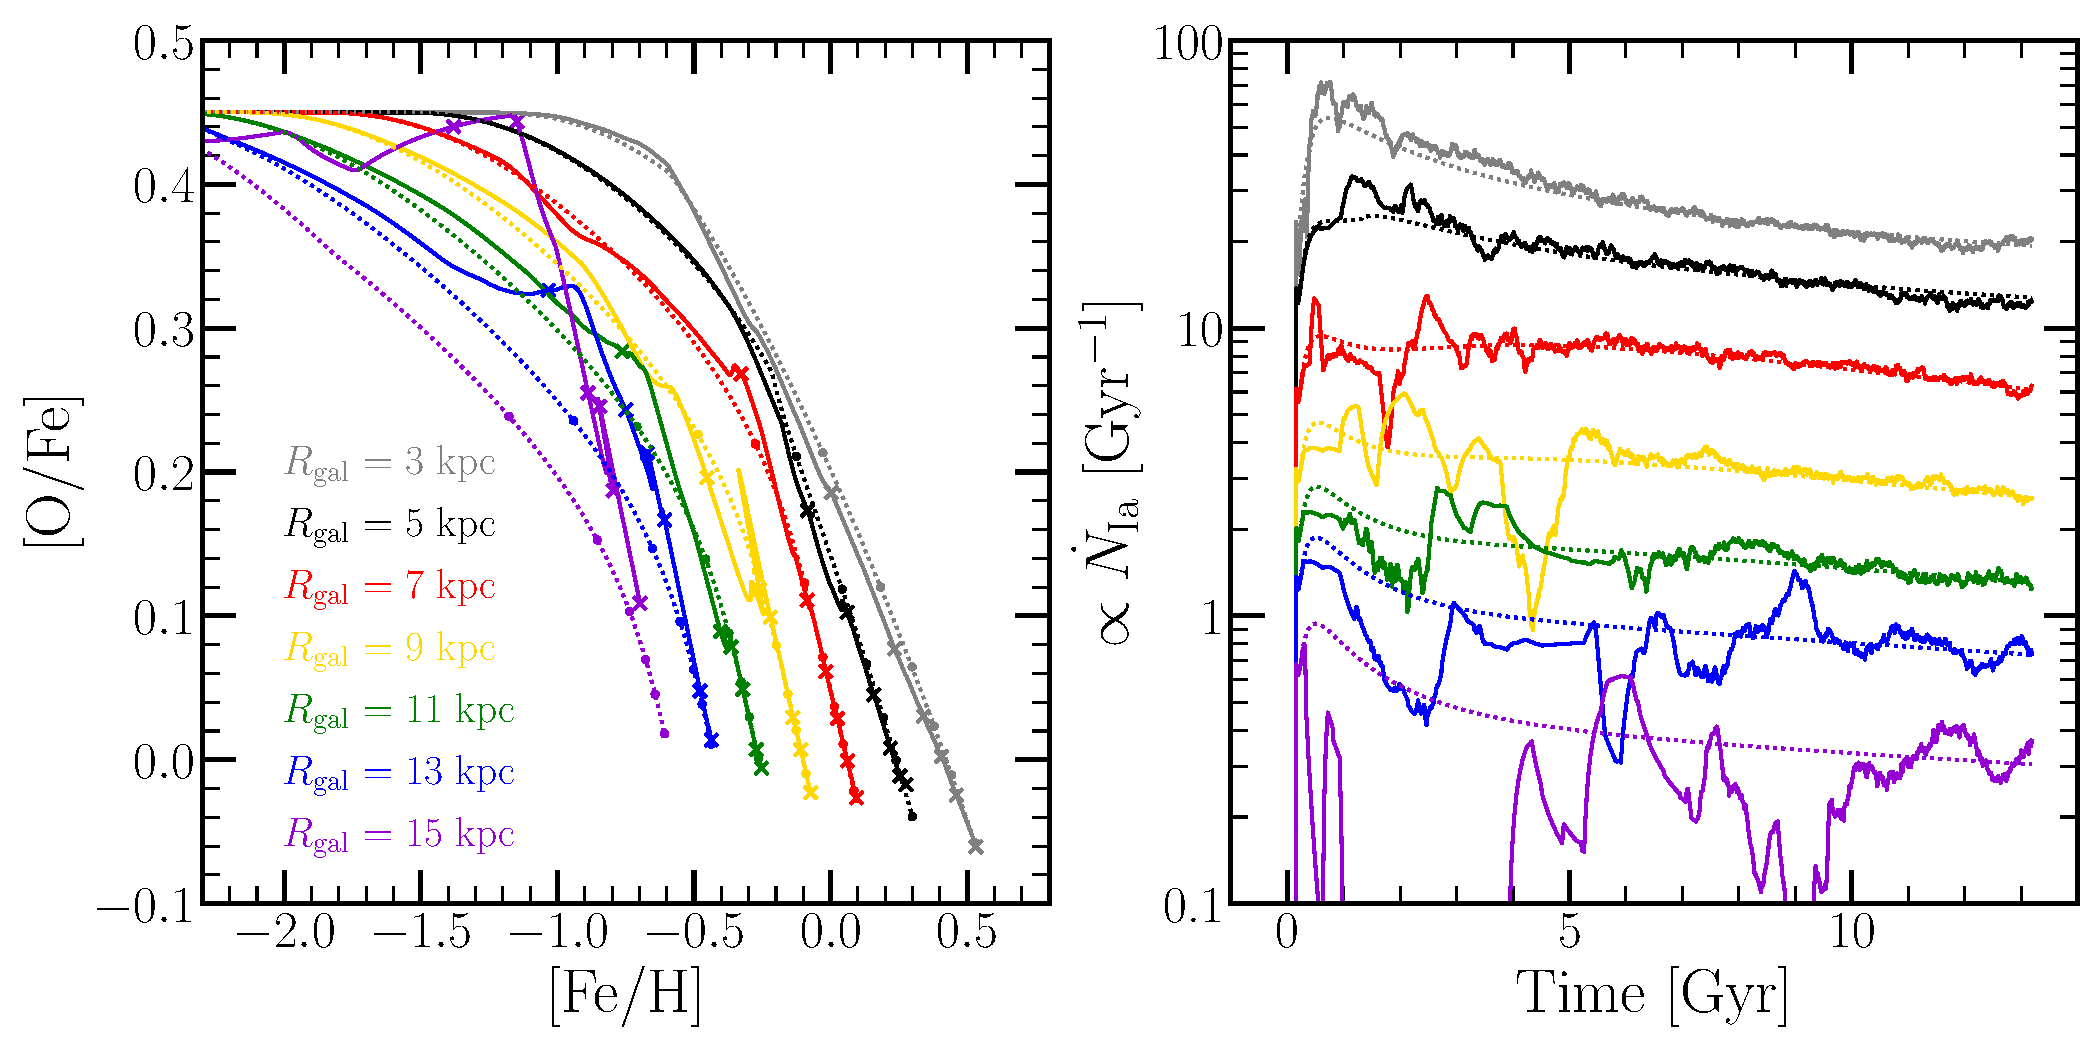
\includegraphics[scale = 0.42]{tracks.pdf} 
\caption{\textbf{Left}: Gas phase evolutionary tracks in the [O/Fe]-[Fe/H] 
plane for our inside-out SFH with either post-processing (dotted lines) or 
diffusion (solid lines) migration models. We plot tracks for seven annuli, 
colour-coded according to their Galactocentric radius and denoted by the 
legend in the lower-left. We mark simulation times of 2, 4, 6, 8, 10, and 12.2 
Gyr in X's for the diffusion model and points for the post-processing model. 
\textbf{Right}: As a function of simulation time, a proxy for the SN Ia rate 
using the total time-derivative of the Fe mass in a given annulus, calculated 
by subtracting the contribution from recycling and CCSN enrichment and adding 
back that lost to star formation and outflows. We show these rates for the 
same annuli as in the left-hand panel, multiplying them by various prefactors 
to improve clarity. } 
\label{fig:tracks} 
\end{figure*} 

We continue by assessing the impact of stellar migration on the gas-phase 
tracks in the [O/Fe]-[Fe/H] plane. To this end, we compare the predictions of 
our post-processing migration model, which has stars stay at their radii of 
birth until they instantaneously migrate at the present day, and our diffusion 
model, which has stars migrating continuously with a~$\sqrt{\text{age}}$ 
dependence. In the left-hand panel of Fig.~\ref{fig:tracks}, we plot the 
[O/Fe]-[Fe/H] tracks at several radii assuming the inside-out 
SFH, with post-processing shown in dotted lines and the diffusion in solid 
lines. We also mark simulation times of 2, 4, 6, 8, 10, and 12.2 Gyr on each 
track for reference. 
\par 
We note first and foremost that there are considerable differences between the 
two sets of tracks, particularly at high [O/Fe]. We demonstrate here that this 
arises out of variability in SN Ia rates caused by the time-dependent radial 
migration of the diffusion model. From our~\texttt{VICE} outputs, the total 
time derivative of the Fe mass in a given annulus can be obtained by its change 
across a single timestep. By then subtracting the CCSN contribution (known 
exactly given our adopted yield and the SFR), approximately correcting for 
recycling, and adding back that which was lost to star formation and outflows, 
we obtain a simple estimate of the rate of Fe production by SNe Ia. 
\par 
We plot this proxy as a function of simulation time in the right-hand panel of 
Fig.~\ref{fig:tracks}, with dotted and solid lines again denoting 
post-processing and diffusion migration models and the same colour-coding as in 
the left-hand panel; we have also multiplied these curves by various prefactors 
to improve clarity. As expected, the post-processing model predicts a SN Ia 
rate which is a smooth function of time at a given~$R_\text{gal}$. The diffusion 
model on the other hand exhibits significant variability on~$\sim$Gyr 
timescales; the time-averaged SN Ia rate tends to follow the post-processing 
prediction, but the instantaneous rates do not agree. A close comparison allows 
one to realize that whenever one of the tracks in the left-hand panel shows 
higher (lower) [O/Fe] at a given [Fe/H], there is an excess (deficit) in the SN 
Ia rate at a similar time and radius. Early times in the~$R_\text{gal}$ = 15 
kpc annulus illustrates a rather extreme example whereby the SN Ia rate is 
effectively zero for nearly 3 Gyr. We also note that the fractional amplitude 
of the variability increases with~$R_\text{gal}$; the log-scaled y-axis makes 
this clear. This makes sense physically because the lower stellar number 
density in the outer Galaxy means it would be much more susceptible to sampling 
noise. That is, a single star migrating has a larger fractional impact at 
large radii than small radii. 

% fig 9 
\begin{figure*} 
\centering 
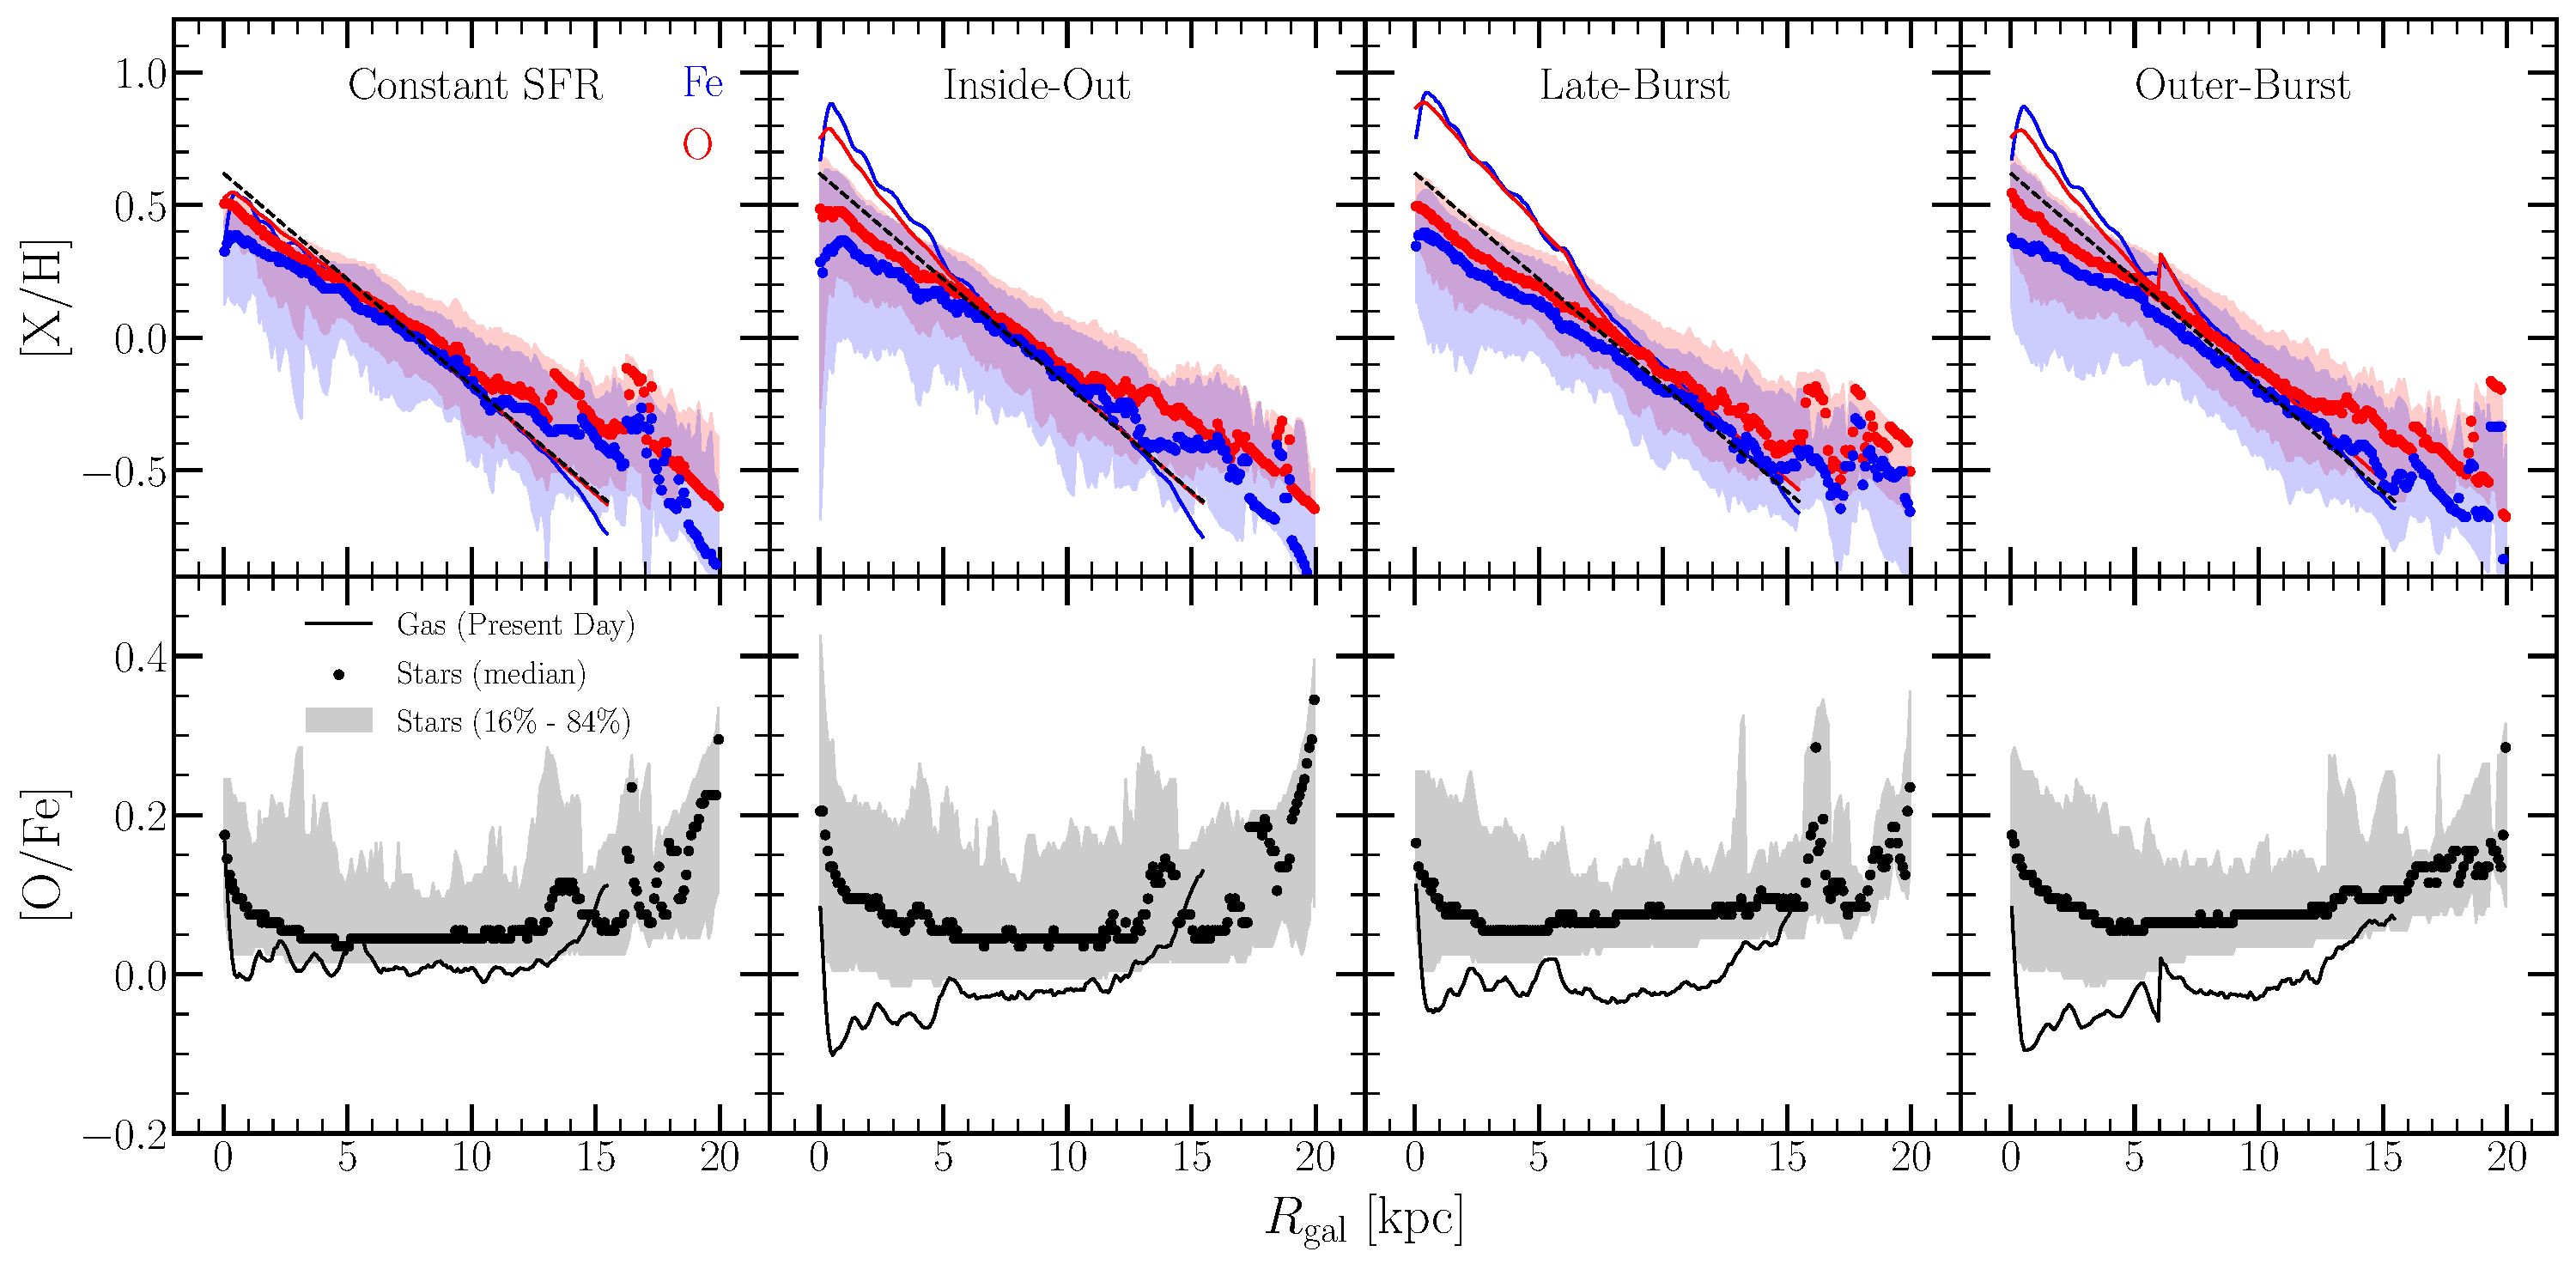
\includegraphics[scale = 0.32]{metallicity_gradient.pdf} 
\caption{Radial abundance gradients in [O/H] (top, red), [Fe/H] (top, blue), 
and [O/Fe] (bottom) for our four fiducial SFHs - constant (far left), 
inside-out (left-middle), late-burst (right-middle), and outer-burst (far 
right). We plot the gas-phase abundance at the present day as a function of 
Galactocentric radius in solid lines. Stars denote the median of the stellar 
MDF of the 100-pc width annulus at a given radius, with shaded regions marking 
the 16th and 84th percentiles thereof. Black lines in the top panels denote our 
target [$\alpha$/H] gradient of mode([$\alpha$/H]) = +0.3 at~$R_\text{gal}$~= 
4 kpc with a slope of -0.08 kpc$^{-1}$. } 
\label{fig:metallicity_gradient} 
\end{figure*} 

Although one may expect the rates predicted by the two migration models to 
agree based on the dynamical argument that a star migrating outward should be 
balanced by a star migrating inward due to the conservation of energy, the SN 
Ia rate depends not only on stellar number density but also on the masses and 
ages of the stellar populations. While an inwardly migrating star should be 
balanced dynamically by an outwardly migrating one, the SN Ia rate is 
unaffected only when the two have masses and ages such that the SN Ia DTD has 
the same value for both stars. Fluctuations in the SN Ia rate at these 
amplitudes can be understood through a comparison of the timescales associated 
with radial migration and SN Ia events. In Fig.~\ref{fig:h277_decomposition}, 
we plotted the distribution of final radii in bins of birth radius and age, 
which are used in driving stellar migration in our models (see discussion in~\S 
\ref{sec:methods:h277}). From this, we noted that~$\sim$40\% of~\texttt{h277} 
star particles migrated beyond their birth radius by the time they were~$\sim$2 
Gyr old. Though our adopted form differs slightly in detail, if the SN Ia DTD 
is a~$\sim t^{-1}$ power-law with a minimum delay time of~$\sim$100 Myr 
\citep{Maoz2012, Maoz2017}, then there should be similar numbers of SN Ia 
events with delay times between 1 and 10 Gyr as there are between 100 Myr and 1 
Gyr. While our~$R_\text{gal}$~= 15 kpc annulus is something of an extreme 
example, when one realizes that this means~$\sim$half of SN Ia progenitors may 
move significantly beyond their birth radius, the amplitude of the variability 
seen in the right-hand panel of Fig.~\ref{fig:tracks} is not surprising. The 
fact that >10\% of events are seen at >10 kpc from their host galaxies in the 
ASAS-SN bright SN catalog~\citep{Holoien2019} adds qualitative, observational 
support to the argument that SN Ia progenitors may often form at significantly 
different radii than where the explosions are observed. 
\par 
We thus argue that the radial migration of nucleosynthetic yields can occur 
alongside stellar migration for delayed sources. Though we do not investigate 
this effect for such elements in this paper, it would be reasonable to expect 
similar predictions for s-process elements produced in AGB stars like carbon, 
nitrogen, strontium, yttrium, and zirconium as well as r-process elements from 
neutron star mergers if the associated DTD is sufficiently long. What we really 
learn from this investigation is that tracks are not simple functions when 
stellar migration is taken into account. To first order, they're characterized 
by the late-time equilibrium abundance and the value of~$\tau_\star$~setting 
the position of the ``knee''~\citep{Weinberg2017}, though migration causes 
noticeable variations which should depend on the details of the adopted 
dynamical history. In~\S~\ref{sec:obs_comp:age_alpha}, we demonstrate that 
this is a means with which truly young, super-solar [$\alpha$/Fe] stars in the 
solar neighborhood can be explained theoretically. 
\par 
We continue with an investigation into the radial abundance gradients predicted 
by our models. To some extent, a gradient is built into our models via a 
scaling of the mass loading factor~$\eta$~with Galactocentric radius (see 
discussion in~\S~\ref{sec:methods:yields}). In parameterizing the 
$\eta-R_\text{gal}$ scaling, we assumed our constant SFH model and the 
associated equilibrium abundance for alpha elements. Like the surface density 
gradient, we also assumed that stellar migration does not alter the overall 
form. We plot the radial [O/H] and [Fe/H] gradients predicted by all our 
models in the top row of Fig.~\ref{fig:metallicity_gradient}, and the [O/Fe] 
gradients in the bottom row. In all panels, stars denote the median abundance 
in each annulus, and the shaded region denotes the 16th and 84th percentiles of 
the MDF in that zone; solid lines denote the gas-phase gradient at the present 
day. Although we built the gradient into our models based on the mode abundance, 
we illustrate them here according to the median; we find that with annuli as 
narrow as~$\Delta R_\text{gal}$~= 100 pc, the mode is a sufficiently noisy 
statistic to introduce noticeably more scatter in this relation. Nonetheless we 
have verified that it follows the trend implied by our target gradient, 
illustrated by the solid black line. The median gradient for all of our model 
SFHs follows a slightly shallower trend than the mode, which is expected when 
the metallicity distribution is skew-negative in the inner Galaxy and 
skew-positive in the outer Galaxy. 
\par 
We note that our models indeed recover an~$R_\text{gal}$-[O/H] relation 
resembling that which was adopted. As was the case for the surface density 
gradient (see discussion in~\S~\ref{sec:methods:surface_density_gradient}), 
stellar migration appears to only introduce scatter. While our procedure for 
setting setting the abundance gradient did not consider Fe, our models predict 
it to follow a gradient similar to that of O. We further note that all SFHs 
predict an [O/Fe] gradient which is relatively flat at all radii, steepening 
only at very small and very large~$R_\text{gal}$. The trend toward higher 
[O/Fe] beyond~$R_\text{gal}$~= 15.5 kpc is expected, since this is the radius 
at which we shut off star formation; all stellar populations at these radii at 
the present day formed in the disc and migrated there, meaning this region of 
space in our model is populated only by stars sufficiently old to have migrated 
such distances. Because they're old, they also tend to be~$\alpha$-enhanced. 
This is consistent with the findings of~\citet{RadburnSmith2012}, who argue 
that the outskirts of the NGC 7793 disc formed largely out of stellar 
migration. {\color{red} Observational reference on the increase in [O/Fe] at 
small~$R_\text{gal}$? Maybe~\citet{Hayden2015}, but I'm not sure.} 
\par 
We also note that our models predict differences between the stellar and 
present-day gas-phase gradients which are sensitive to the adopted SFH. In the 
constant SFH model, the gas-phase gradient follows the mode abundance by 
construction. In the inside-out, late-burst, and outer-burst models, the 
ISM at small~$R_\text{gal}$~is considerably more metal-rich than the stars at 
similar radii. The late-burst model shows the largest difference; this is a 
consequence of the starburst at small~$R_\text{gal}$, an effect which is absent 
in the outerburst model. In accretion-induced starbursts, re-enrichment can 
briefly produce super-equilibrium abundances in the gas-phase which then decay 
back to the equilibrium abundance as the SFR declines~\citep{Johnson2020}. This 
effect can also be seen in the outer-burst model; at~$R_\text{gal}$ slightly 
larger than 6 kpc where the starburst did occur, the abundances are larger than 
at slightly less than 6 kpc, where the star burst did~\textit{not} occur. 
Altogether, these differences are reflective of the notion that the stellar 
abundance gradient is sensitive to stars of all ages and thus the entire star 
formation history, while the gas-phase gradient is more reflective of 
enrichment over the previous depletion time. 

\subsection{Metallicity Distributions Functions} 
\label{sec:obs_comp:mdfs} 

% fig 10 
\begin{figure} 
\centering 
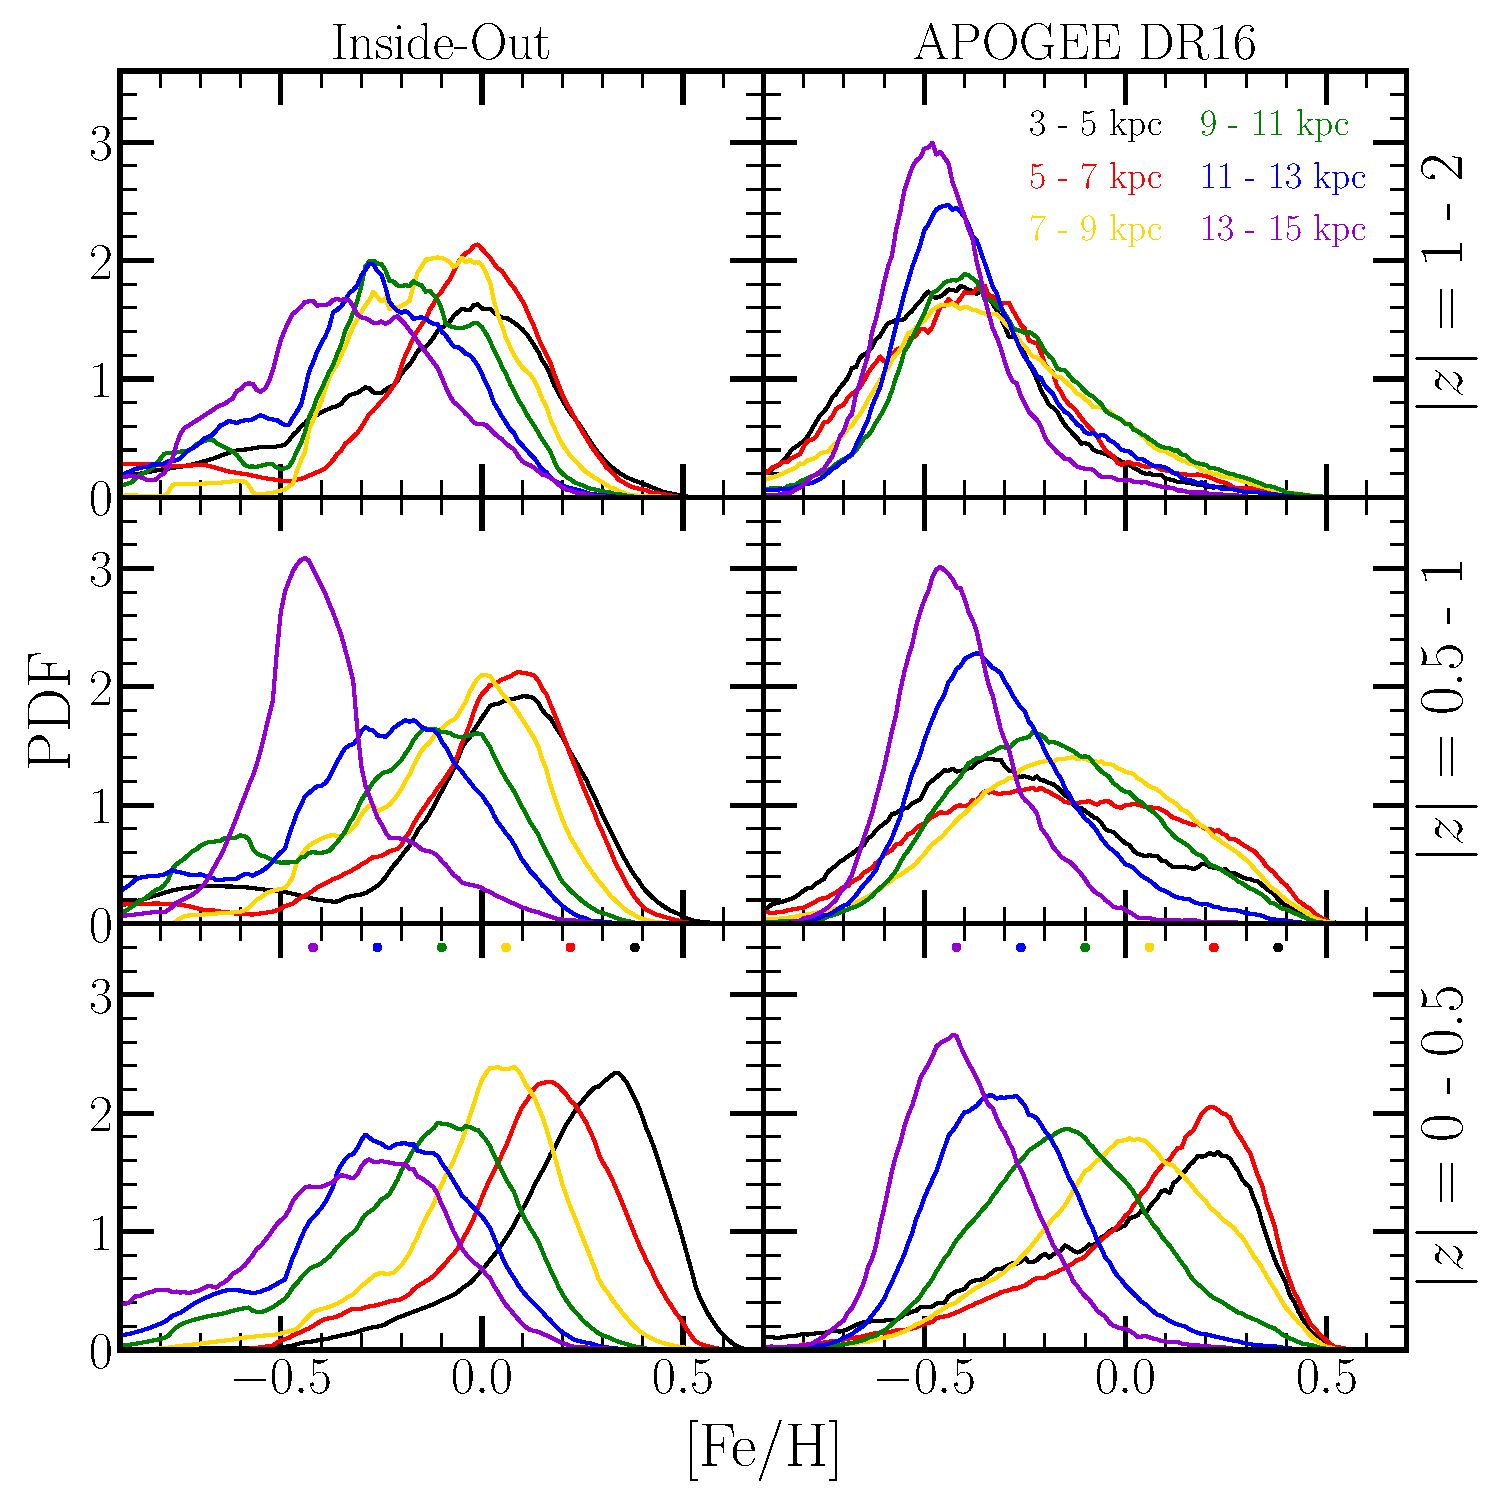
\includegraphics[scale = 0.34]{mdf_3panel_fe.pdf} 
\caption{Metallicity distribution functions (MDFs) in [Fe/H] predicted by our 
fiducial, inside-out model (left) and as observed in APOGEE DR16 (right), for 
stars and simulated stellar populations with present-day~$\left|z\right|$~= 0 - 
0.5 kpc (bottom), 0.5 - 1 kpc (middle), and 1 - 2 kpc (top). MDFs are shown in 
bins of Galactocentric radius: 3 - 5 kpc (black), 5 - 7 kpc (red), 7 - 9 kpc 
(yellow), 9 - 11 kpc (green), 11 - 13 kpc (blue), and 13 - 15 kpc (purple). 
The points near the top of the bottom panels denote what the mode abundance 
would be if it followed out target gradient of [Fe/H] = +0.3 at~$R_\text{gal}$ 
= 4 kpc with a slope of -0.08 kpc$^{-1}$ exactly, assuming the inner radius of 
each bins (i.e. there is no point plotted for 15 kpc). All distributions are 
smoothed with a box-car width of [Fe/H]~$\pm$~0.1 for clarity. } 
\label{fig:mdf_3panel_fe} 
\end{figure} 

% fig 11 
\begin{figure} 
\centering 
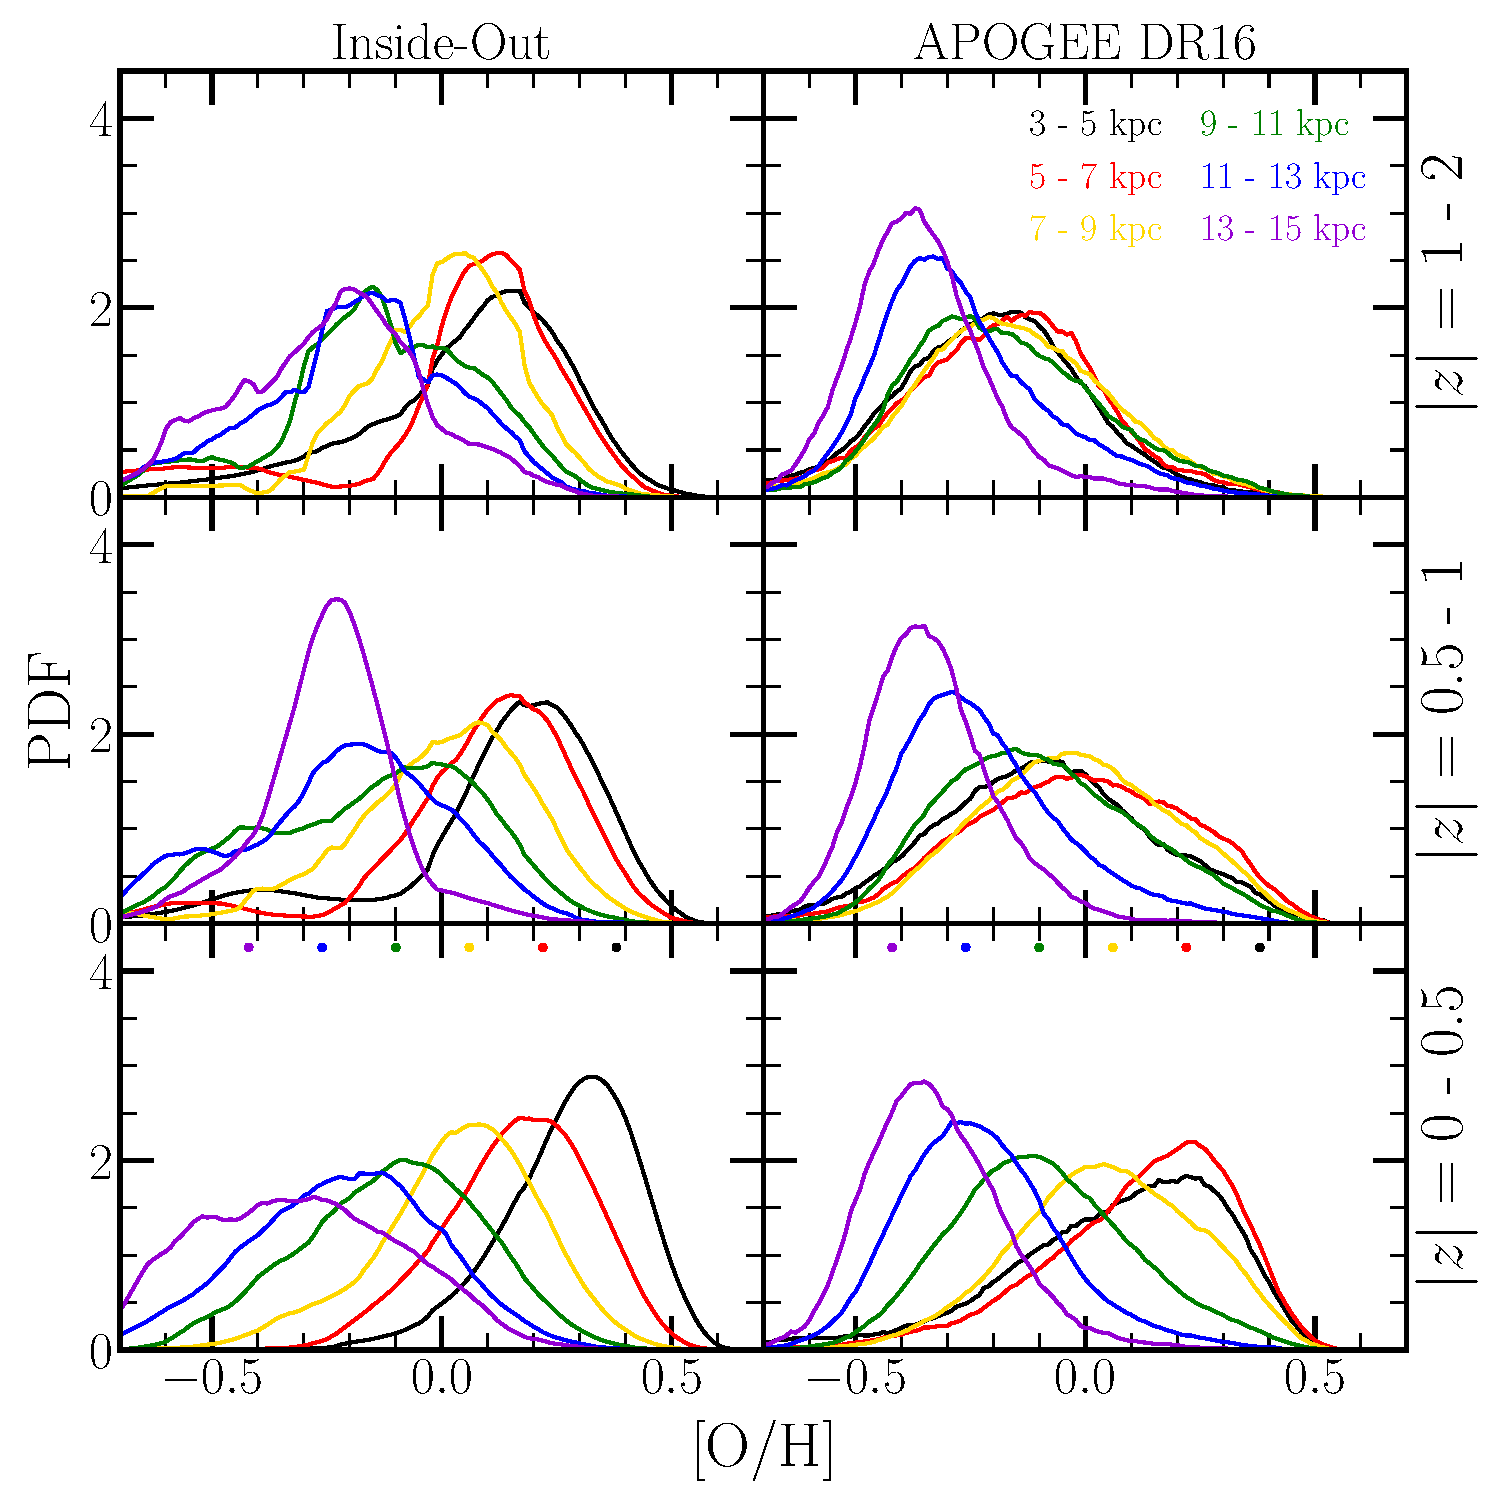
\includegraphics[scale = 0.34]{mdf_3panel_o.pdf} 
\caption{The same as Fig.~\ref{fig:mdf_3panel_fe}, but for [O/H]. } 
\label{fig:mdf_3panel_o} 
\end{figure} 

Metallicity distribution functions (MDFs) and how they vary with Galactic 
region are one of the core predictions of chemical evolution models. In this 
section, we compare our model predicted MDFs to those observed in the 16th 
data release of APOGEE (DR16;~\citealp{Ahumada2020, Majewski2017}). The 
data are reduced using the APOGEE Stellar Parameters and Chemical Abundances 
Pipeline (ASPCAP;~\citealp{Holtzman2015, GarciaPerez2016}). For further details 
of the APOGEE survey, a brief summary can be found in~\S~2 of 
\citet{Weinberg2019}. We restrict our sample to stars with effective 
temperatures of 4000 K~$\leq T_\text{eff} \leq$~4600 K, surface gravities of 
1.0~$\leq \log g \leq$~2.5, and signal-to-noise ratios of at least 100. These 
cuts ensure that our sample consists of stars on the upper red giant branch, 
safely excluding red clump stars to avoid obvious systematics in the 
abundance distributions. 
\par 
In the disc midplane, stars as observed by APOGEE are known to exhibit mode 
[$\alpha$/H] and [Fe/H] abundances that depend on Galactocentric radius, with a 
skew-negative distribution in the inner Galaxy and skew-positive in the outer 
Galaxy~\citep{Hayden2015, Weinberg2019}. Off the midplane, the MDFs converge on 
[$\alpha$/H]~$\approx$~[Fe/H]~$\approx$~-0.5. This result is replicated in the 
right-hand column of panels~\ref{fig:mdf_3panel_fe} and~\ref{fig:mdf_3panel_o}. 
The left-hand columns show the distributions predicted by our fiducial 
inside-out model. We note that these replicate the qualitative scaling of the 
mode [O/H] and [Fe/H] with present-day Galactocentric radius, though our APOGEE 
data suggest that the 3 - 5 and 5 - 7 kpc bins share a common mode abundance. 
This was also seen in~\citet{Hayden2015}. Our models do not predict this 
detail; this could indicate that we have incorrectly parameterized outflows in 
the inner Galaxy (see discussion regarding our scaling of the mass loading 
factor~$\eta$~with~$R_\text{gal}$ in~\S~\ref{sec:methods:yields}). We would 
expect a flat [X/H] gradient and MDFs with similar modes if we simply chose it 
to be so by letting~$\eta$~be constant at small~$R_\text{gal}$. Another 
possibility is the cessation of star formation in these regions; by tracing 
products of star formation such as HII regions~\citep{Guesten1982}, supernova 
remnants~\citep{Leahy1989}, and pulsars (\citealp*{Lyne1985}; 
\citealp{Case1998}), the surface density of star formation~$\dot{\Sigma}_\star$ 
in the Milky Way is known to reach a maximum at~$R_\text{gal} \approx$~4 kpc 
(see Fig. 1 of~\citealt{Peek2009} and Fig. 2 of~\citealt{Fraternali2012}). Our 
models by construction predict~$\dot{\Sigma}_\star$ to decrease monotonically 
with~$R_\text{gal}$~(see Fig.~\ref{fig:evol}). If the Milky Way has begun 
quenching star formation, a process which is believed to begin in the centres 
of galaxies at this mass~\citep[e.g.][]{Ellison2020b}, then fewer stars would 
form in the most metal-rich regions than do in our models, cutting off the MDF 
at high [O/H] and [Fe/H]. 
\par 
Beyond the midplane, our models fail to fully replicate the convergence of the 
MDFs at [X/H]~$\approx$~-0.5. The observed MDF at small radii shfits from 
skew-negative with a metal-rich mode to skew-positive with a metal-poor 
mode with increasing~$\left|z\right|$. In our model predicted MDFs for small 
$R_\text{gal}$, the mode does shift to lower abundances, but not to the same 
extent as in the observed sample, and with minimal change in skewness. 
Although the model predicts a portion of the effect, it cannot account for the 
entire~$\left|z\right|$-dependence of the MDF shape in the inner Galaxy. 

\subsection{[O/Fe] distributions in Bins of [Fe/H]} 
\label{sec:obs_comp:ofe_dists} 
In this section we compare our predicted [O/Fe] distributions in various 
Galactic regions to those recently published in~\citet{Vincenzo2021a}. As in our 
\S~\ref{sec:obs_comp:mdfs}, they also make use of APOGEE DR16 
\citep{Ahumada2020, Majewski2017}, and impose a similar set of cuts on 
effective temperature, surface gravity, and signal-to-noise (see their~\S~2). 
These distributions are estimates of the~\textit{intrinsic} [O/Fe] 
distributions that, when 
convolved with observational uncertainties and the APOGEE selection function, 
would resemble the observed MDFs like those in~\citet{Hayden2015}. We show the 
distributions predicted by our fiducial model in~$\Delta$[O/Fe] = 0.04 bins 
across 15 Galactic regions in comparison to the~\citet{Vincenzo2021a} 
distributions shown in dashed lines in Fig.~\ref{fig:ofe_mdfs_insideout}. 
Galactic regions 
are defined by a range in~$R_\text{gal}$, shown in columns and denoted at the 
top of the figure, and a range in~$\left|z\right|$, shown in rows and denoted 
in text in the left-hand column. We show this comparison for two bins in 
[Fe/H], colour-coded according to the legend in the top-right panel. 

\begin{figure*} 
\centering 
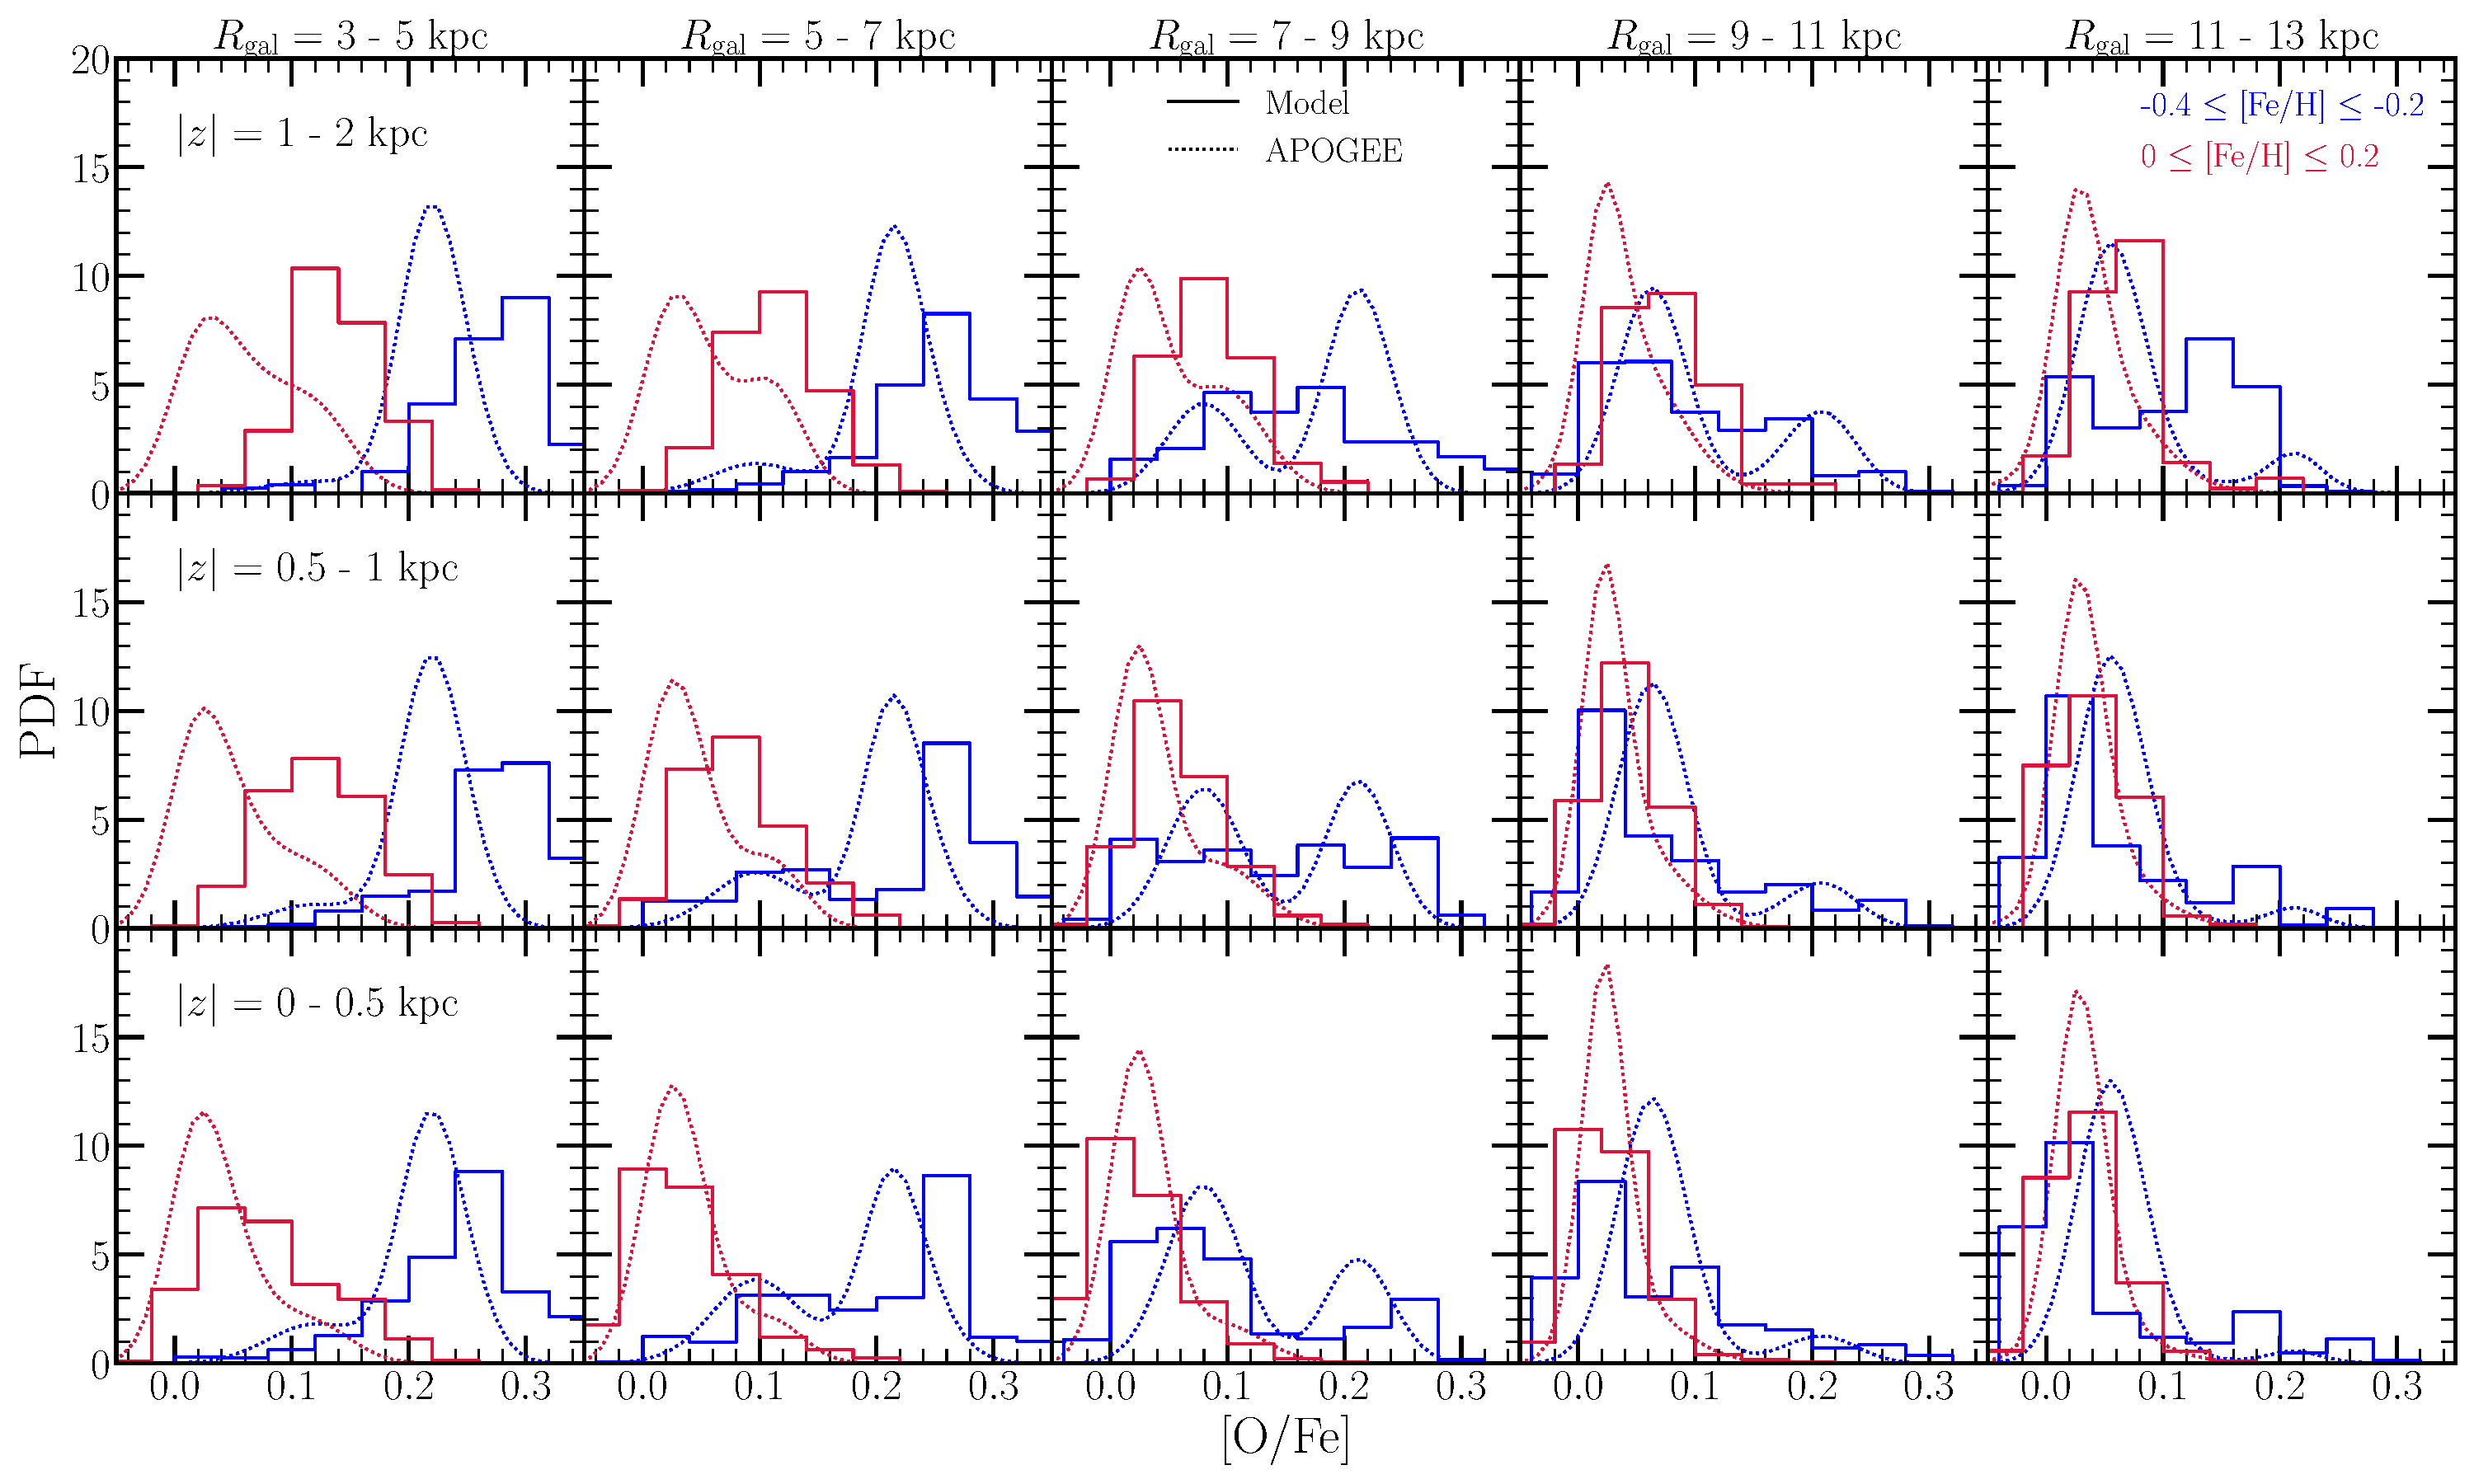
\includegraphics[scale = 0.32]{ofe_mdfs.pdf} 
\caption{Predicted distributions in [O/Fe] in 15 Galactic regions and in two 
bins in [Fe/H]. Columns correspond to bins in~$R_\text{gal}$, denoted at the 
top of each column. Rows correspond to bins in~$\left|z\right|$, denoted in 
text in the left-hand column. Distributions are color-coded according to the 
[Fe/H] the sample is drawn from, denoted by the legend in the upper right 
panel. Solid lines represent that predicted by our inside-out SFH in 
$\Delta$[O/Fe] = 0.04 bins, while dashed lines correspond to the fits to the 
APOGEE DR16 data presented in~\citet{Vincenzo2021a}, which quantify the 
intrinsic distributions accounting for observational uncertainties and the 
APOGEE selection function. } 
\label{fig:ofe_mdfs_insideout} 
\end{figure*} 

Finding similar results for all of our SFHs, we note that our model adequately 
reproduces the broad nature of the [O/Fe] distributions at fixed [Fe/H] seen in 
the APOGEE data. Some distributions in a specific Galactic region and [Fe/H] 
bin show a bimodality in decent agreement with the observations (e.g. the 
-0.4~$\leq$~[Fe/H]~$\leq$~-0.2 bin at~$R_\text{gal}$~= 7 - 9 kpc and 
$\left|z\right|$ = 1 - 2 kpc), but this is not true of all Galactic regions in 
both metallicity bins. Instead, the principle failure of our model is that it 
overpredicts the number of intermediate [O/Fe] stars. 
\par 
In the inner Galaxy, our model overestimates the mode [O/Fe] to some extent for 
both [Fe/H] bins, but the difference is larger for the higher of the two. This 
discrepancy also increases with increasing~$\left|z\right|$. At fixed 
$R_\text{gal}$, the~\citet{Vincenzo2021a} distributions show two peaks which do 
not change with~$\left|z\right|$; only their relative heights vary. This is 
an assumption built into the model, but the agreement with the APOGEE data is 
good. However, this is a region of the Galaxy where there aren't many APOGEE 
stars. At~$\left|z\right|$ = 1 - 2 kpc for ~$R_\text{gal}$ = 3 - 5 and 5 - 7 
kpc, the~\citet{Vincenzo2021a} model is fit to 31 and 17 stars, respectively. In 
comparison, there are 109 in the solar annulus, and all other bins have >75 
stars involved in the fit. It's possible the observed distributions shift 
slightly to higher [$\alpha$/Fe], but at most at the~$\lesssim$~0.05 level 
(see their Fig. 11). 
\par 
If this discrepancy persists in subsequent APOGEE data releases which will 
better characterize the distributions in these regions, it's possible the 
origin is tied to the Sagittarius dwarf. The~\texttt{h277} simulation, which 
drives stellar migration in our models (see discussion in~\S 
\ref{sec:methods}), did not have such an accretion event. With its most recent 
major merger occurring at a redshift of~$z \approx$~3, this galaxy has 
previously been selected for investigation expressly because of its quiescent 
merger history~\citep[e.g.][]{Zolotov2012}. N-body models for the tidal 
disruption of the Sagittarius dwarf, on the other hand, suggest pericentric 
passages around 6.5, 4.5, 2.75, 1, and 0.1 Gyr ago~\citep{Law2010}. In addition 
to potentially triggering episodes of star formation 
\citep[e.g.][]{RuizLara2020}, more frequent pericentric passages of a massive 
satellite could kinematically heat low-[$\alpha$/Fe] disc stars to higher 
$\left|z\right|_\text{max}$~orbits. Such effects are not a component of the 
dynamical history of~\texttt{h277}; this is one instance where running our 
models with a different hydrodynamical simulation's star particles may be an 
enlightening comparison. 
\par 
The notion that an [$\alpha$/Fe] dichotomy can arise out of radial migration 
alone traces back to~\citet{Schoenrich2009}, and was later explored by 
\citet{Nidever2014} and recently by~\citet{Sharma2020}. This however suggests 
that an inside-out star formation history combined with stellar migration is not 
conducive to predicting this observed result, even when a recent starburst is 
added. The primary failure being an overpredicted frequency of intermediate 
[$\alpha$/Fe] stars, this could point to a number of things. If the bimodality 
is to arise out of inside-out Galaxy evolution and stellar migration alone, 
then the transition between high- and low-$\alpha$ sequences needs to occur 
faster than it does in these models. The analytic arguments of 
\citet{Weinberg2017} suggest that the approach to equilibrium occurs on the 
order of the SFE timescale~$\tau_\star$ (see~\S~\ref{sec:methods:sfe}). 
Since we've adopted a star formation law which is motivated by observational 
results, the failure of these models to reproduce the observed dichotomy 
suggests that the typical SFE timescales as observed are not short enough to 
explain such a fast transition. This would imply that either the Milky Way 
occupied a special place in the scatter of the observed 
$\dot{\Sigma}_\star-\Sigma_\text{g}$ relation at a time early in its 
evolutionary history, or the bimodality arose out of alternative pathways. 
Under our current assumptions, the simplest way to decrease the frequency of 
intermediate [$\alpha$/Fe] stars is to simply shut off (or turn down) star 
formation when the ISM is at such a composition. This is an indication 
that two-infall evolutionary histories~\citep[e.g.][]{Chiappini1997, 
Chiappini2001, Romano2010, Grisoni2017, Noguchi2018, Palla2020, Spitoni2016, 
Spitoni2018, Spitoni2019a, Spitoni2020, Spitoni2021} would improve the 
agreement between our model predictions and the observed distributions. 

\subsection{The Age-[$\alpha$/Fe] Relation} 
\label{sec:obs_comp:age_alpha} 
In this section, we assess the predicted age-[O/Fe] relations of our models, 
using the results of~\citet{Feuillet2019} as the observational benchmark; their 
stellar age measurements are based on isochrone matching. While we made 
use of APOGEE DR16 data in comparing our model predictions to the observed 
MDFs~\citep[][see~\S~\ref{sec:obs_comp:mdfs}]{Ahumada2020, Majewski2017}, they 
made use of APOGEE DR14 stars for which parallax measurements are available 
from Gaia~\citep{Abolfathi2014, GaiaDR2}. With their spatial and quality cuts, 
the final 
sample consisted of 77,562 stars. In bins of [O/Fe], they assume a gaussian 
log age distribution, fitting the mean and standard deviation to the stars in 
that bin. Because they assume a gaussian, they would report an equal mean 
and median log age. This means that a one-to-one comparison of our model 
predictions to their results is not free of nuance, because they predict 
log age distributions which are highly non-gaussian at fixed [O/Fe]. 
\par 
The stellar populations from our simulations have different masses; this 
necessitates weighting the age-distributions by present-day mass, because that 
scales with the number of stars that a model stellar population represents. We 
therefore adopt the 50th percentile of the mass-weighted age distribution in a 
bin of [O/Fe] as the characteristic age to compare to the~\citet{Feuillet2019} 
measurements. We refer to this quantity as the mass-weighted median age. 

% fig 13 
\begin{figure*} 
\centering 
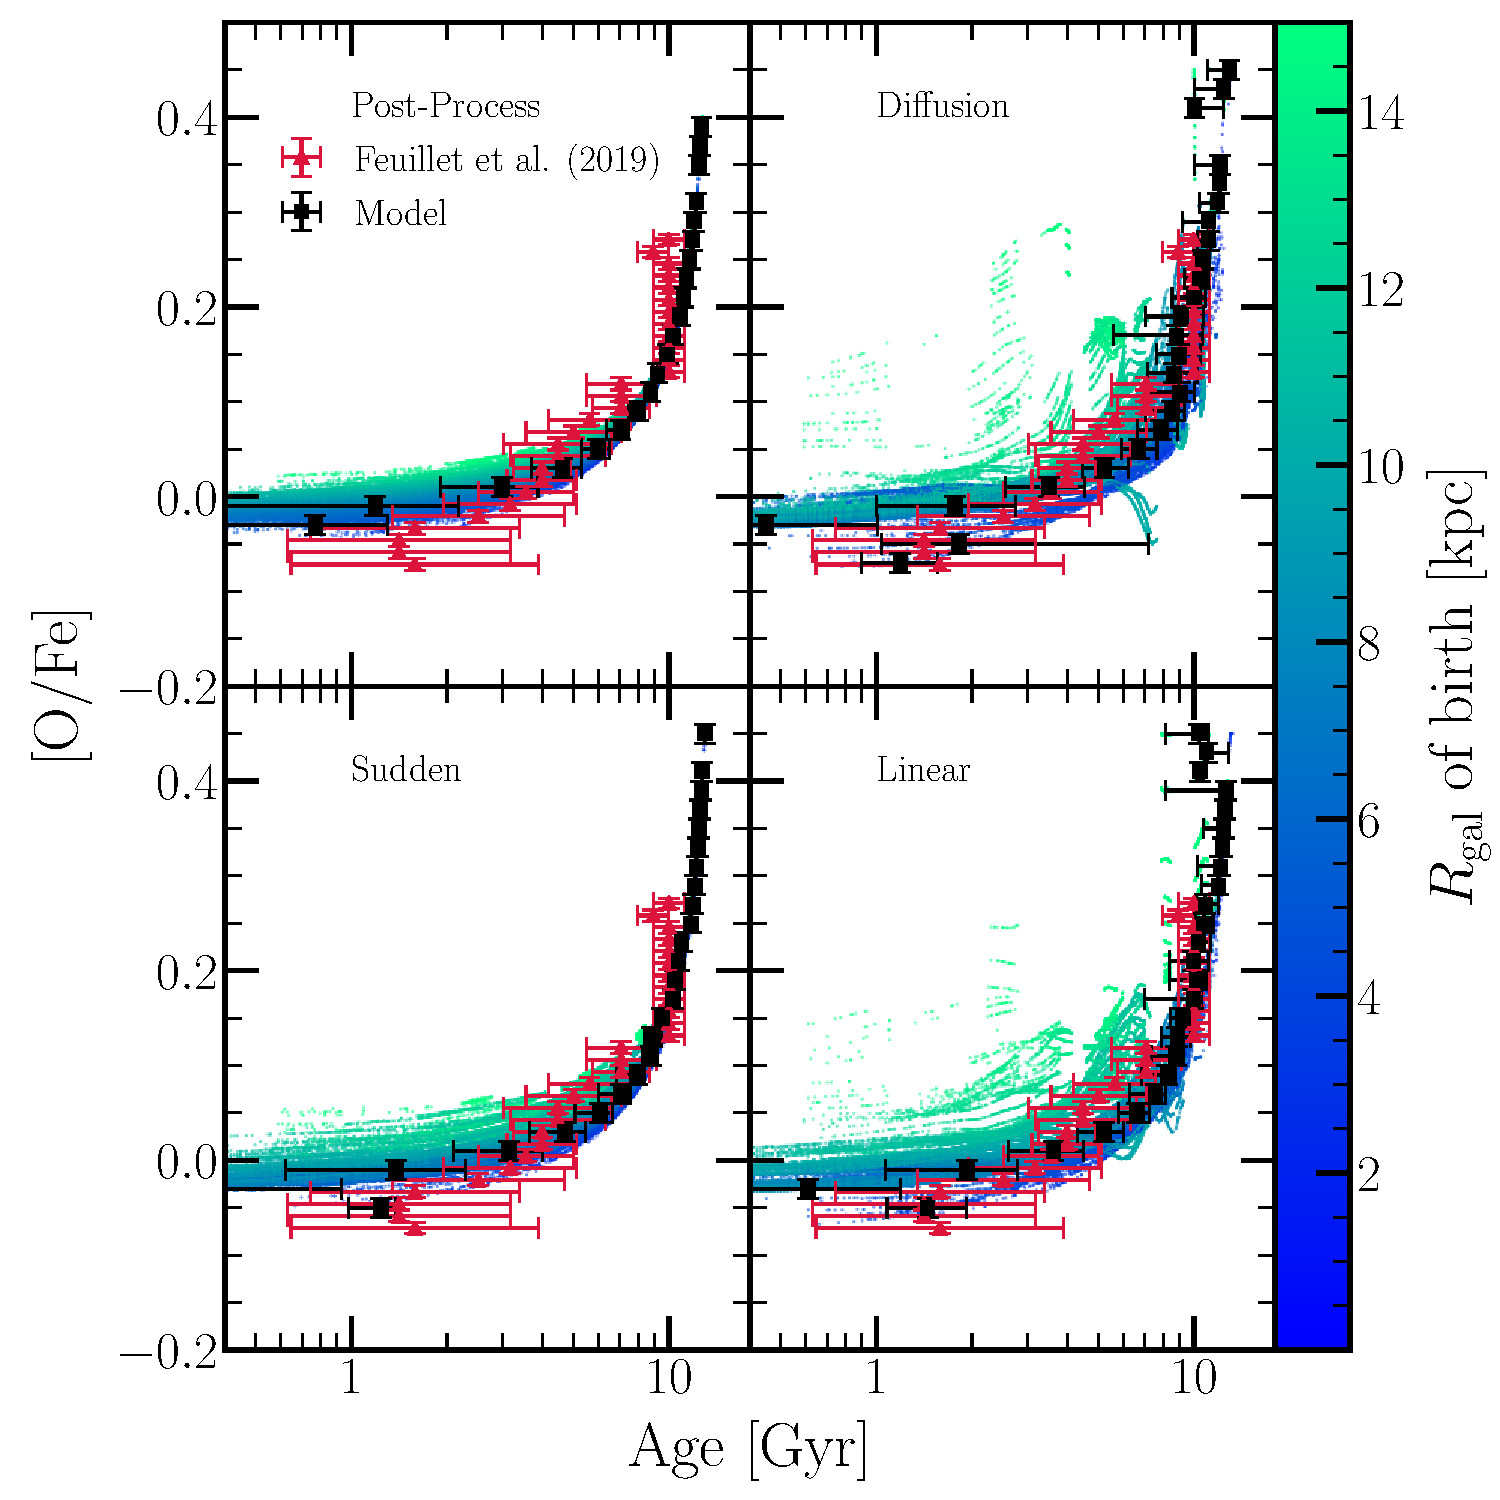
\includegraphics[scale = 0.34]{age_ofe_migration_comparison.pdf} 
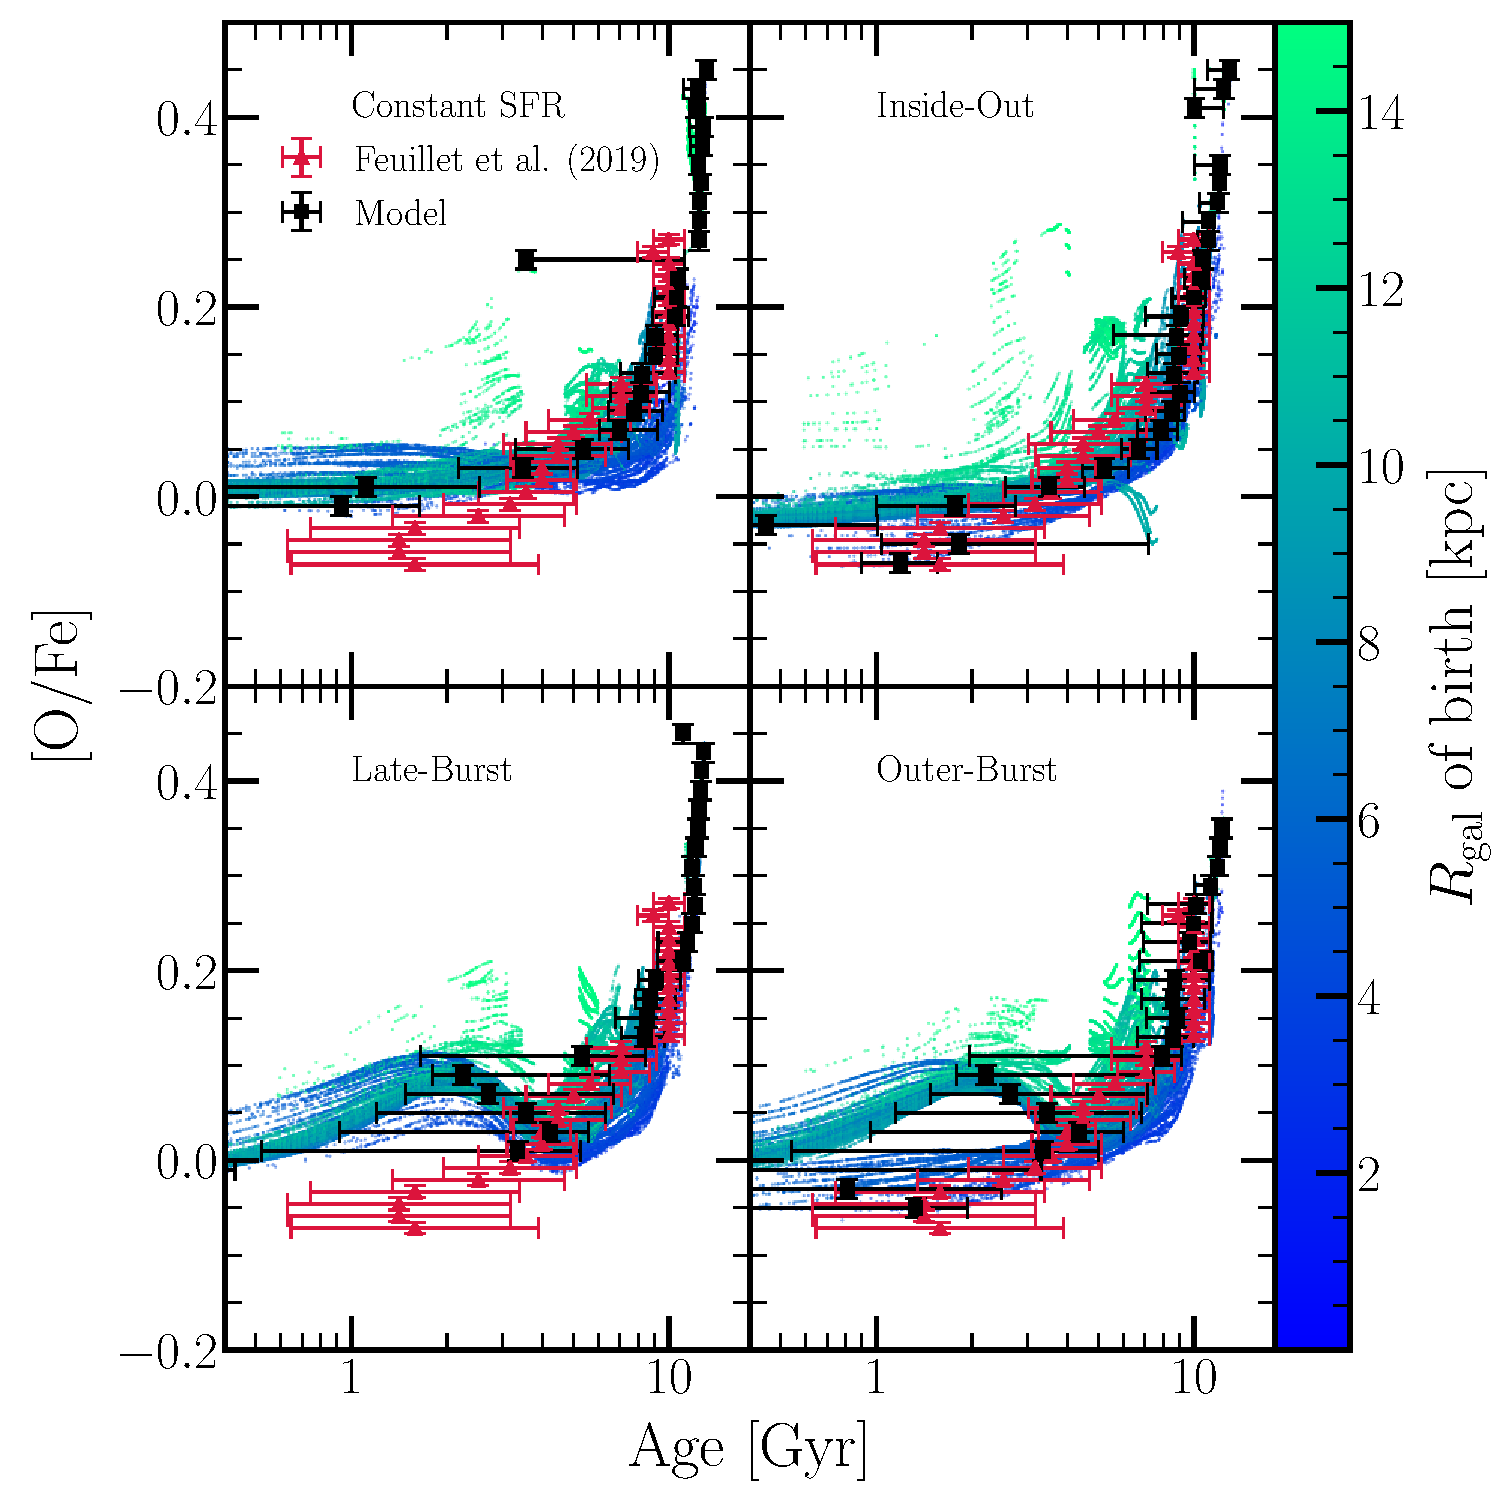
\includegraphics[scale = 0.34]{age_ofe_sfh_comparison.pdf} 
\caption{
\textbf{Left}: A comparison of the predicted age-[O/Fe] relation for the solar 
annulus ($R_\text{gal}$ = 7 - 9 kpc and~$\left|z\right|$ = 0 - 0.5 kpc) between 
the post-processing (upper left), diffusion (upper right), sudden (lower left), 
and linear (lower right) migration models, assuming our inside-out SFH. 
\textbf{Right}: The same as the left-hand panels, instead comparing the impact 
of our constant (upper left), inside-out (upper right), late-burst (lower left), 
and outer-burst (lower right) SFHs, assuming diffusion migration. In all panels, 
red triangles and error bars denote the observed mean age and dispersion 
thereof in bins of [O/Fe] as reported by~\citet{Feuillet2019}; here we include 
only the bins containing at least 15 stars. Black squares denote the 
mass-weighted median age in 0.02-dex bins in [O/Fe] predicted by our models, 
with error bars denoting the 16th and 84th percentiles of the mass-weighted 
age distribution in those bins. Points in the background denote each individual 
stellar population from the model with a final position in the solar annulus, 
colour-coded according to their Galactocentric radius of birth. 
}
\label{fig:age_alpha} 
\end{figure*} 

In the left-hand set of panels of Fig.~\ref{fig:age_alpha}, we compare the 
age-[O/Fe] relation in the solar annulus ($R_\text{gal}$~= 7 - 9 kpc and 
$\left|z\right|\leq$~0.5 kpc) predicted by our four migration models to the 
\citet{Feuillet2019} measurements, shown in red triangles. We mark the 
mass-weighted median age in bins of [O/Fe] in each model with black squares, 
and plot for reference in the background each individual stellar population in 
the solar annulus, colour-coded according to its Galactocentric radius of birth. 
\par 
We note that the inside-out SFH, assumed by all four of the models illustrated 
here, provides a reasonable description of the age-[O/Fe] relation as observed 
in APOGEE. We also note that each model for the time-dependence of stellar 
migration predicts differing amounts of scatter in the age-[O/Fe] relation. 
Diffusion has the most, followed by linear, then sudden, and lastly 
post-processing. We interpret this as a consequence of the variability in the 
SN Ia rate as a function of radius and time caused by time-dependent migration 
(see Fig.~\ref{fig:tracks} and associated discussion near the beginning of~\S 
\ref{sec:obs_comp}). When the SN Ia rate is higher or lower than expected given 
the SFH of an annulus, then the Fe abundance in that zone will increase or 
decrease accordingly. This can occur if there is a significant net gain or loss 
of SN Ia progenitors in a given time interval due to time-dependent migration. 
The gas-phase [O/Fe] then decreases or increases in turn, and the stars which 
form out of that gas inherit these compositions. When migration is taken into 
account and stellar populations are mixed as a consequence, the observational 
signature is intrinsic scatter in the age-[$\alpha$/Fe] relation. 
\par 
All of the models in the left-hand set of panels predict a correlation between 
mass-weighted median age and [O/Fe] in good agreement the~\citet{Feuillet2019} 
measurements assuming the inside-out SFH. This suggests that the population 
averaged trend is unaffected by stellar migration. However, only the diffusion 
and linear migration models predict a population of young ($\lesssim$~4 Gyr), 
[$\alpha$/Fe]~$\approx$~+0.1 - 0.2 stars in the solar neighbourhood. These 
stars are a part of the noticeable upward scatter in the relationship, and we 
therefore interpret their origin to be the same as the scatter itself - they 
formed in a region of the Galactic ISM at a time when it was particularly 
alpha-enhanced due to a rather lasting deficit in SN Ia events. These stars 
then migrated to the solar annulus, where they showed up in the APOGEE data 
when stellar ages were measured using carbon-to-nitrogen ratios 
\citep{Martig2016}, isochrone matching~\citep{Feuillet2018, Feuillet2019}, 
and with the asteroseismic ages of the origin APOKASC catalog 
\citep{Chiappini2015, SilvaAguirre2018, Pinsonneault2014}. 
\par 
\citet{SilvaAguirre2018} demonstrate that the observed young $\alpha$-rich 
stars in the solar annulus have kinematics similar to the rest of the 
high-$\alpha$ population, and suggested this may be the result of stellar 
mergers or mass transfer events. This would produce a population of truly old 
stars masquerading as young stars. In a sample of 51 young, $\alpha$-rich 
red giants,~\citet{Hekker2019} demonstrate that a portion of these stars have 
carbon-to-nitrogen ratios consistent with mass transfer events, but that others 
do not, indicating they're either truly young stars or the result of mergers 
on the main sequence. As far as we know, the mechanism discussed here is the 
first theoretical explanation of the origin of these stars. We note 
additionally that under this explanation, the young~$\alpha$-rich stars are 
not so much $\alpha$-rich as they are Fe-poor, and form overwhelmingly at 
large~$R_\text{gal}$ where the SN Ia rate is most variable (see discussion in 
\S~\ref{sec:obs_comp:gradient}). 
\par 
In the right-hand set of panels in Fig.~\ref{fig:age_alpha}, we 
compare the model predictions of our four different SFHs, assuming our 
diffusion migration model, with the same plotting scheme and colour-coding as 
in the left-hand panels. We note that the constant and inside-out SFHs describe 
the data the best. Although our e-folding timescales for star formation are 
sufficiently long at large~$R_\text{gal}$ such that there is little difference 
between the constant and inside-out SFHs there anyway (see discussion in~\S 
\ref{sec:methods:sfhs}), our constant SFH is idealized and of purely 
theoretical interest, making the inside-out model the more likely of the two. 
Below [O/Fe]~$\approx$~+0.1, the~\citet{Feuillet2019} data seem to follow a 
slightly steeper age-[$\alpha$/Fe] relation than our inside-out model 
predicts. This could point to any number of things being an inaccuracy in our 
models: the detailed form of the SFH or the SN Ia DTD, our supernova yields, 
or observational [O/Fe] errors, all of which are plausible. 
\par 
We note that our starburst models, both late-burst and outer-burst, disagree 
with the~\citet{Feuillet2019} measurements. The late starburst produces a 
population of young, $\alpha$-rich stars due to the perturbed ratio of core 
collapse to type Ia supernova rates~\citep{Johnson2020}. With the starburst 
occurring in a substantial fraction of the ISM in both models, the result is an 
increase in the bulk [$\alpha$/Fe] for young stars which simply is not seen in 
the observed sample. The effect is strong enough that at [O/Fe]~$\approx$~+0.1, 
both models considerably overpredict the width of the distribution, 
simultaneously predicting a mass-weighted median age many times the standard 
deviation younger than observed. This discrepancy is of interest, because these 
models were motivated by the observational results of~\citet{Mor2019} and 
\citet{Isern2019} which suggest such a recent starburst. Although our 
functional forms differ from what they reported in detail, they're reasonable 
descriptions of the measurements within the error bars. This suggests that the 
results of~\citet{Mor2019} and~\citet{Isern2019} are at odds with chemical 
evolution models of the Milky Way. If the Galaxy truly experienced a recent 
starburst, then something not included in our models had to prevent this global 
increase in [$\alpha$/Fe]. 

% fig 14 
\begin{figure*} 
\centering 
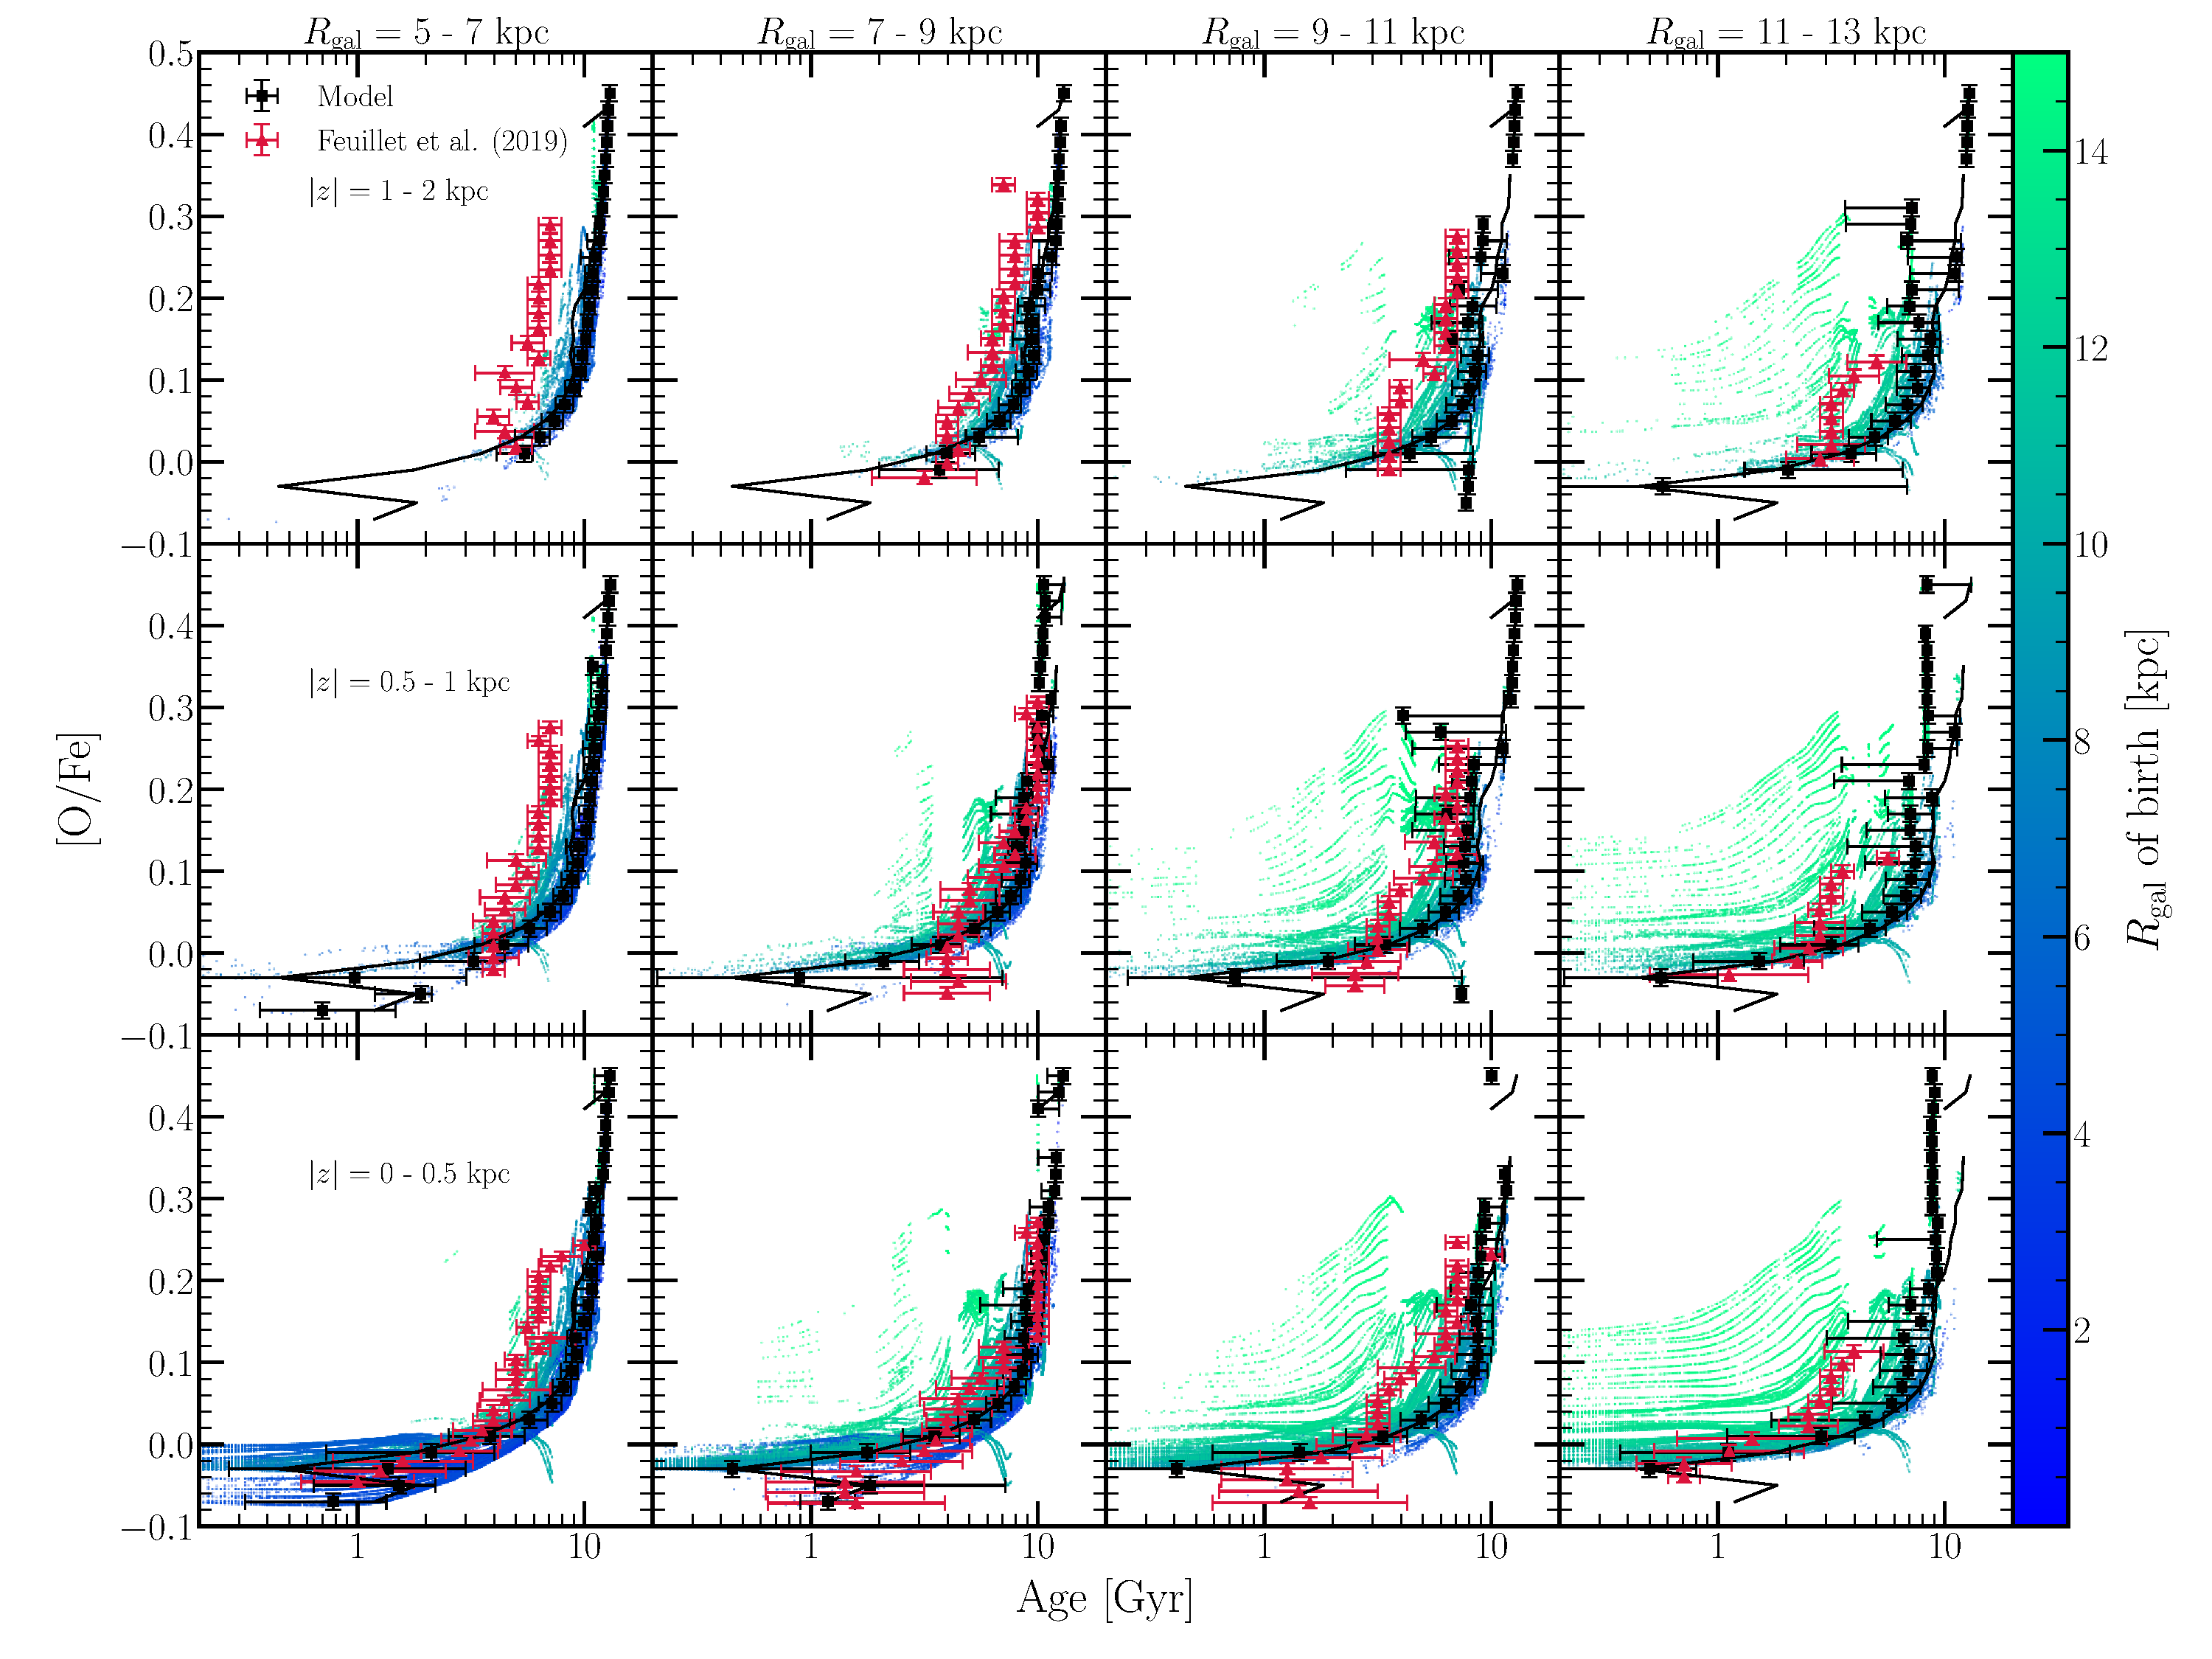
\includegraphics[scale = 0.32]{age_alpha_regions.pdf} 
\caption{The age-[O/Fe] relation in 12 Galactic regions predicted by our 
inside-out SFH. Bins in Galactocentric radius are shown in columns, and labeled 
at the top. Bins in the height~$\left|z\right|$ above/below the disc midplane 
are shown in rows, noted in the left-hand column. Red triangles, black squares, 
error bars, and background points are as in Fig.~\ref{fig:age_alpha} for the 
corresponding Galactic region. The solid black line connects the black squares 
in the bottom, left-middle panel, and is replicated elsewhere for reference. } 
\label{fig:age_alpha_regions} 
\end{figure*} 

In Fig.~\ref{fig:age_alpha_regions}, we extend the comparison of our base-line, 
inside-out model and the observations of~\citet{Feuillet2019} to other 
Galactic regions. We visualize the data there in the same manner as for 
previous figures in this section. While the inside-out model shows the best 
agreement with the observed result in the solar annulus, there are some mild 
discrepancies for stars farther from the sun.~\citet{Feuillet2019} report ages 
for~$\alpha$-rich stars that are younger at large~$R_\text{gal}$ and high 
$\left|z\right|$, though in most cases only by~$\sim$20\%. Our model does not 
capture this effect. To illustrate this, we connect the black squares in the 
panel corresponding to the solar annulus with a black line, and then reproduce 
this line in all panels for reference. If the observational result is correct, 
this is an interesting effect that our model doesn't reproduce in any of the 
variants we've explored. Furthermore, we note that the model overpredicts ages 
at large~$\left|z\right|$. As with the overpredicted [O/Fe] ratios at small 
$R_\text{gal}$, we speculate that this may be tied to the Sagittarius dwarf 
(see discussion in~\S~\ref{sec:obs_comp:ofe_dists}). By using a hydrodynamical 
simulation of a 
galaxy which exhibited more pericentric passages of a massive satellite, more 
young stars may be kinematically heated to high~$\left|z\right|_\text{max}$ 
orbits. This is another instance where running our models with a different 
hydrodynamical simulation's star particles may be an enlightening comparison. 
\par 
We note that the intrinsic scatter in the age-[O/Fe] relation is predicted to 
grow with increasing~$R_\text{gal}$; this can be seen in the error bars on the 
black squares as well as the coloured points. We identify two sources of this 
dependence; the bulk of the scatter, at least at [O/Fe]~$\gtrsim$~+0.05, arises 
from the variability in the SN Ia rates as described in~\S 
\ref{sec:obs_comp:gradient}. Having demonstrated that the SN Ia rate is most 
variable at large~$R_\text{gal}$, the in-situ populations in the outskirts of 
the Galactic disc formed from an ISM whose gas-phase [O/Fe] ratio varied with 
a higher amplitude. Since the observational signature of this variability is 
scatter in the observed age-[O/Fe] relation, our model predicts the most 
intrinsic scatter in Galactic regions where that variability has the highest 
amplitude. Second, the analytic models of~\citet{Weinberg2017} suggest that 
as the e-folding timescale for star formation~$\tau_\text{sfh}$ increases, the 
model-predicted [O/Fe] of the youngest stars increases with a weak dependence. 
With a range of e-folding timescales in our model, this implies a distribution 
of [O/Fe] at age = 0 with nonzero width without considering the migration of 
nucleosynthetic yields. This can be seen in the post-processing model 
predicted age-[O/Fe] relation in Fig.~\ref{fig:age_alpha}. In this pathway, 
scatter is induced by mixing populations that follow age-[O/Fe] relations of 
slightly different normalizations which are nearly flat intrinsically, 
producing a noticeably wide age distribution near solar [O/Fe]. 
\par 
Although the iron-peak is the only class of elements with a delayed 
nucleosynthetic source that we consider in the present paper, we expect similar 
results for other delayed sources with regard to the variability in enrichment 
rates and scatter in age-[X/Y] relations. The details of SN Ia nucleosynthesis 
did not matter in our interpretations in this section; it is based purely on 
the characteristic delay-times of the source and how they compare to the 
timescales of stellar migration. Our models should then find similar 
predictions with, for example, s-process (slow neutron capture) elements like 
carbon, nitrogen, strontium, yttrium, and zirconium produced in asymptotic 
giant branch stars. In fact, using hydrodynamical simulations from the Auriga 
project~\citep{Grand2017},~\citet{vandeVoort2020} find that the intrinsic 
scatter in r-process (rapid neutron capture) abundances increases for models 
with longer characteristic delay times. Although the first observations of a 
binary neutron star merger (GW170817) exhibited an optical counterpart which 
was consistent with being powered by the radioactive decay of r-process 
elements~\citep{Abbott2017, Coulter2017, Drout2017, Pian2017}, it remains 
unclear the extent to which neutron star mergers contribute to r-process 
nucleosynthesis in the universe~\citep{Cote2019, Mishenina2019, Siegel2019, 
vandeVoort2020, Vincenzo2021b}. Although it's likely unfeasible at present due 
to the requirement for high precision abundance measurements of intrinsically 
rare elements in many stars, with future observational capabilities, the 
application of our results as well as~\citet{vandeVoort2020} suggests that the 
intrinsic scatter in r-process abundances may provide constraints on the 
characteristic delay times of such nucleosynthetic events. 

\subsection{The Age-Metallicity Relation} 
\label{sec:obs_comp:amr} 

% fig 15 
\begin{figure} 
\centering 
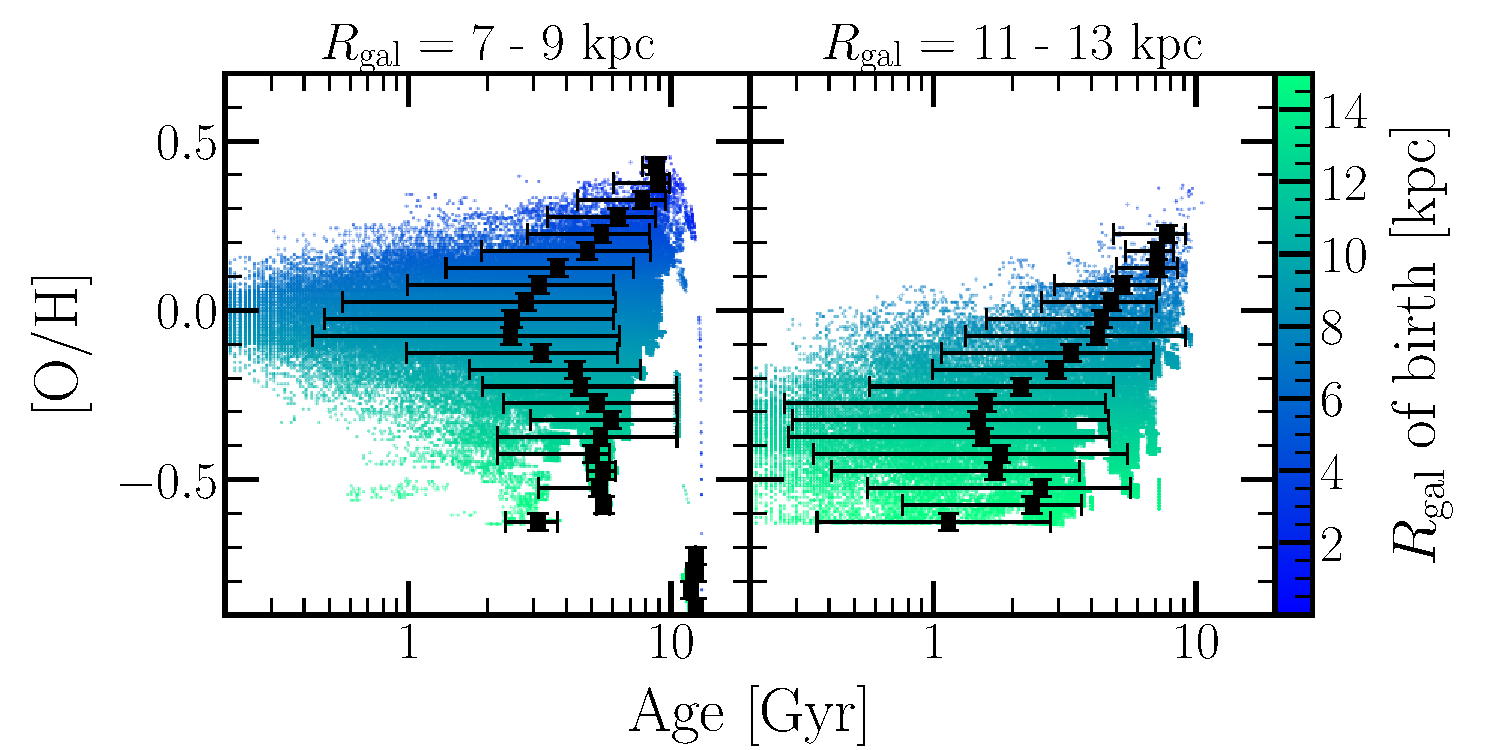
\includegraphics[scale = 0.35]{amr_static_o.pdf} 
\caption{The age-[O/H] relation predicted by our constant SFH model for 
$R_\text{gal}$~= 7 - 9 kpc (left) and 11 - 13 kpc (right). Each panel plots 
only the~$\left|z\right|\leq$~0.5 kpc population. The colored points in the 
background and the black squares with error bars are as in Fig. 
\ref{fig:age_alpha}, but with our binned, model prediction quantified in 
bins of~$\Delta$[O/H] = 0.05. } 
\label{fig:age_oh_static} 
\end{figure} 

Although the age-metallicity relation (AMR) is usually formulated in terms of 
[Fe/H], it is also interesting to quantify the age-[O/H] relation, because it 
is not affected by SN Ia enrichment. The extent to which they differ indicates 
the extent to which the delayed timescale and impact of migration on SN Ia 
enrichment is important in shaping the age-[Fe/H] relation. In Fig. 
\ref{fig:age_oh_static}, we present the age-[O/H] relation predicted by our 
constant SFH model for the~$\left|z\right|\leq$~0.5 kpc population at 
$R_\text{gal}$ = 7 - 9 and 11 - 13 kpc. The black squares with error bars 
denote the mass-weighted median age as in~\S~\ref{sec:obs_comp:age_alpha}, and 
we again plot the individual stellar populations in the background for 
reference, colour-coded according to their Galactocentric radius of birth. We 
omit the~\citet{Feuillet2019} measurements from this figure, because the 
constant SFH model is of purely theoretical interest, removing the effects of 
a time-varying SFH while including the effects of stellar migration. 
\par 
The intrinsic scatter in the observed AMR has previously been interpreted as 
evidence for radial mixing~\citep{Edvardsson1993, Sellwood2002}. In the 
solar neighbourhood,~\citet{Feuillet2018} demonstrate that the most metal-rich 
stars tend to be significantly older than solar metallicity stars. Using the 
\citet{Weinberg2017} analytic models of one-zone chemical evolution, they argue 
that this is the result of old stars born at small~$R_\text{gal}$ where the 
equilibrium abundance is high. Only the old stars are able to migrate to 
the solar neighbourhood due to the time required for such a change in their 
orbital radius. 
\par 
The results of our constant SFH model illustrated in Fig. 
\ref{fig:age_oh_static} extend our understanding of this effect. In both 
regions plotted, the youngest stars form with a composition inherited from the 
local ISM, which in this model, is reflective of the late-time equilibrium 
abundance. At a given age, only stars born in a well-defined region of the 
Galaxy will have had adequate time to migrate to a given present-day radius. 
Since a range of~$R_\text{gal}$ maps directly to a range of metallicity once 
the ISM is arbitrarily close to the equilibrium abundance in our model, this 
necessitates a maximum width of the [O/H] distribution at fixed age. With 
increasing age, the [O/H] distribution then gets wider because any given 
present-day radius samples stars formed at a wider range of~$R_\text{gal}$. 
In Fig.~\ref{fig:age_oh_static}, we indeed see this effect, with the 
colour-coding of the background points making it clear that stellar migration 
is the culprit. In the outer Galaxy, migration has a particularly interesting 
effect in that it only adds old stars above the equilibrium metallicity; in 
the~$R_\text{gal}$ = 11 - 13 kpc region, our model as a consequence predicts 
an AMR where the population-averaged trend where [O/H] is nearly monotonically 
increasing with age. This is entirely backwards from what is expected from 
one-zone models of GCE~\citep[e.g.][]{Andrews2017, Weinberg2017, Johnson2020}. 

% fig 16 
\begin{figure} 
\centering 
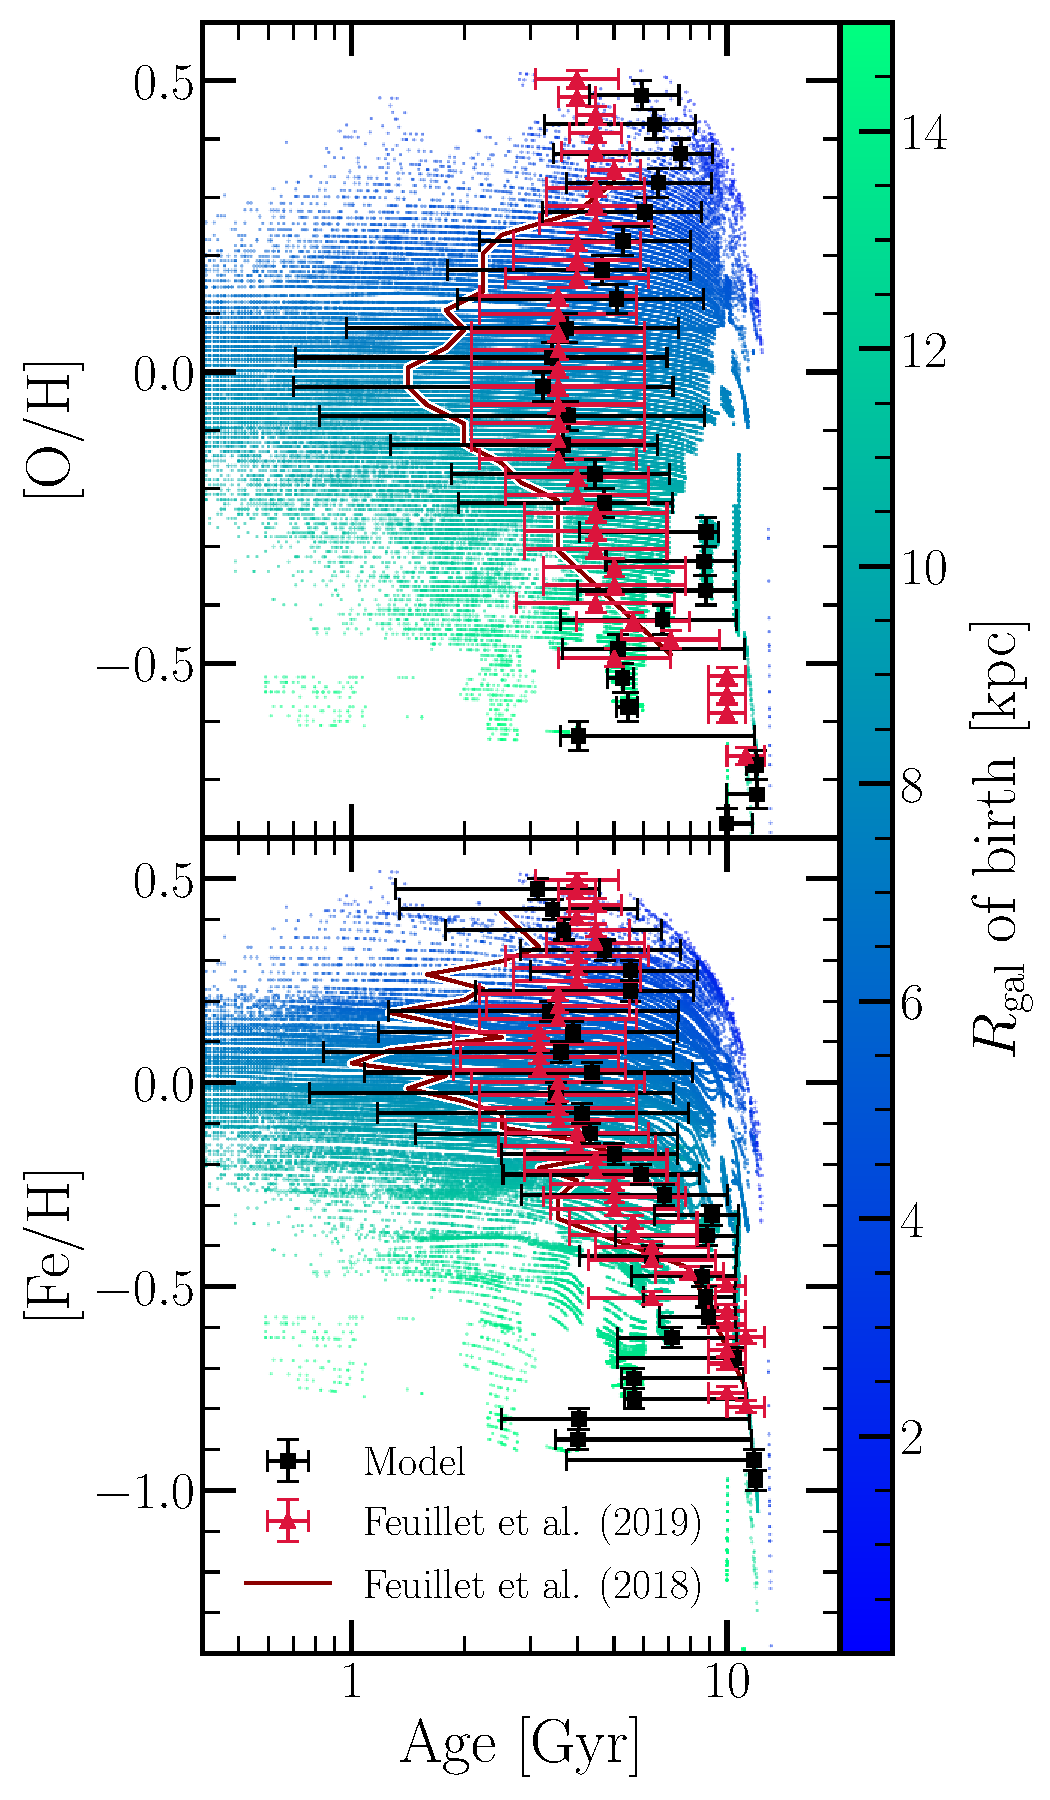
\includegraphics[scale = 0.45]{amr_solar_annulus.pdf} 
\caption{The age-[O/H] (top) and age-[Fe/H] (bottom) relations for the solar 
annulus (i.e.~$R_\text{gal}$ = 7 - 9 kpc,~$\left|z\right|\leq$~0.5 kpc) as 
predicted by our inside-out SFH. Red triangles, black squares, error bars, and 
background points are as in Fig.~\ref{fig:age_alpha}, but with our model 
predicted quantified in bins of~$\Delta$[O/H] =~$\Delta$[Fe/H] = 0.05. For 
comparison, we plot the~\citet{Feuillet2018} measurements in a dark red line, 
omitting the associated uncertainties for visual clarity. } 
\label{fig:amr_solar_annulus} 
\end{figure} 

We continue our assessment of the model-predicted AMR by illustrating in Fig. 
\ref{fig:amr_solar_annulus} the age-[O/H] (top) and age-[Fe/H] (bottom) 
relations predicted for the solar annulus (i.e.~$R_\text{gal}$~= 7 - 9 kpc and 
$\left|z\right|\leq$~0.5 kpc). The red triangles, black squares, coloured 
points, and error bars are as in previous figures in~\S 
\ref{sec:obs_comp:age_alpha}. For reference, we add the solid dark red line, 
which denotes the AMR measured by~\citet{Feuillet2018}. Although our model 
shows decent agreement with the~\citet{Feuillet2019} measurements in the solar 
annulus,~\citet{Feuillet2018} report ages for solar metallicity stars which 
are considerably younger ($\sim$1 - 2 Gyr as opposed to~$\sim$3 - 4 Gyr). 
The~\citet{Feuillet2018} data would suggest our inside-out model requires an 
enhancement in the recent SFR to increase the frequency of young, solar 
metallicity stars. Although our late-burst and outer-burst models include 
such effects, motivated by recent observations suggesting this exact 
evolutionary history~\citep{Mor2019, Isern2019}, the differences between the 
\citet{Feuillet2018} and~\citet{Feuillet2019} measurements are interesting in 
and of themselves. 

% fig 17 
\begin{figure*} 
\centering 
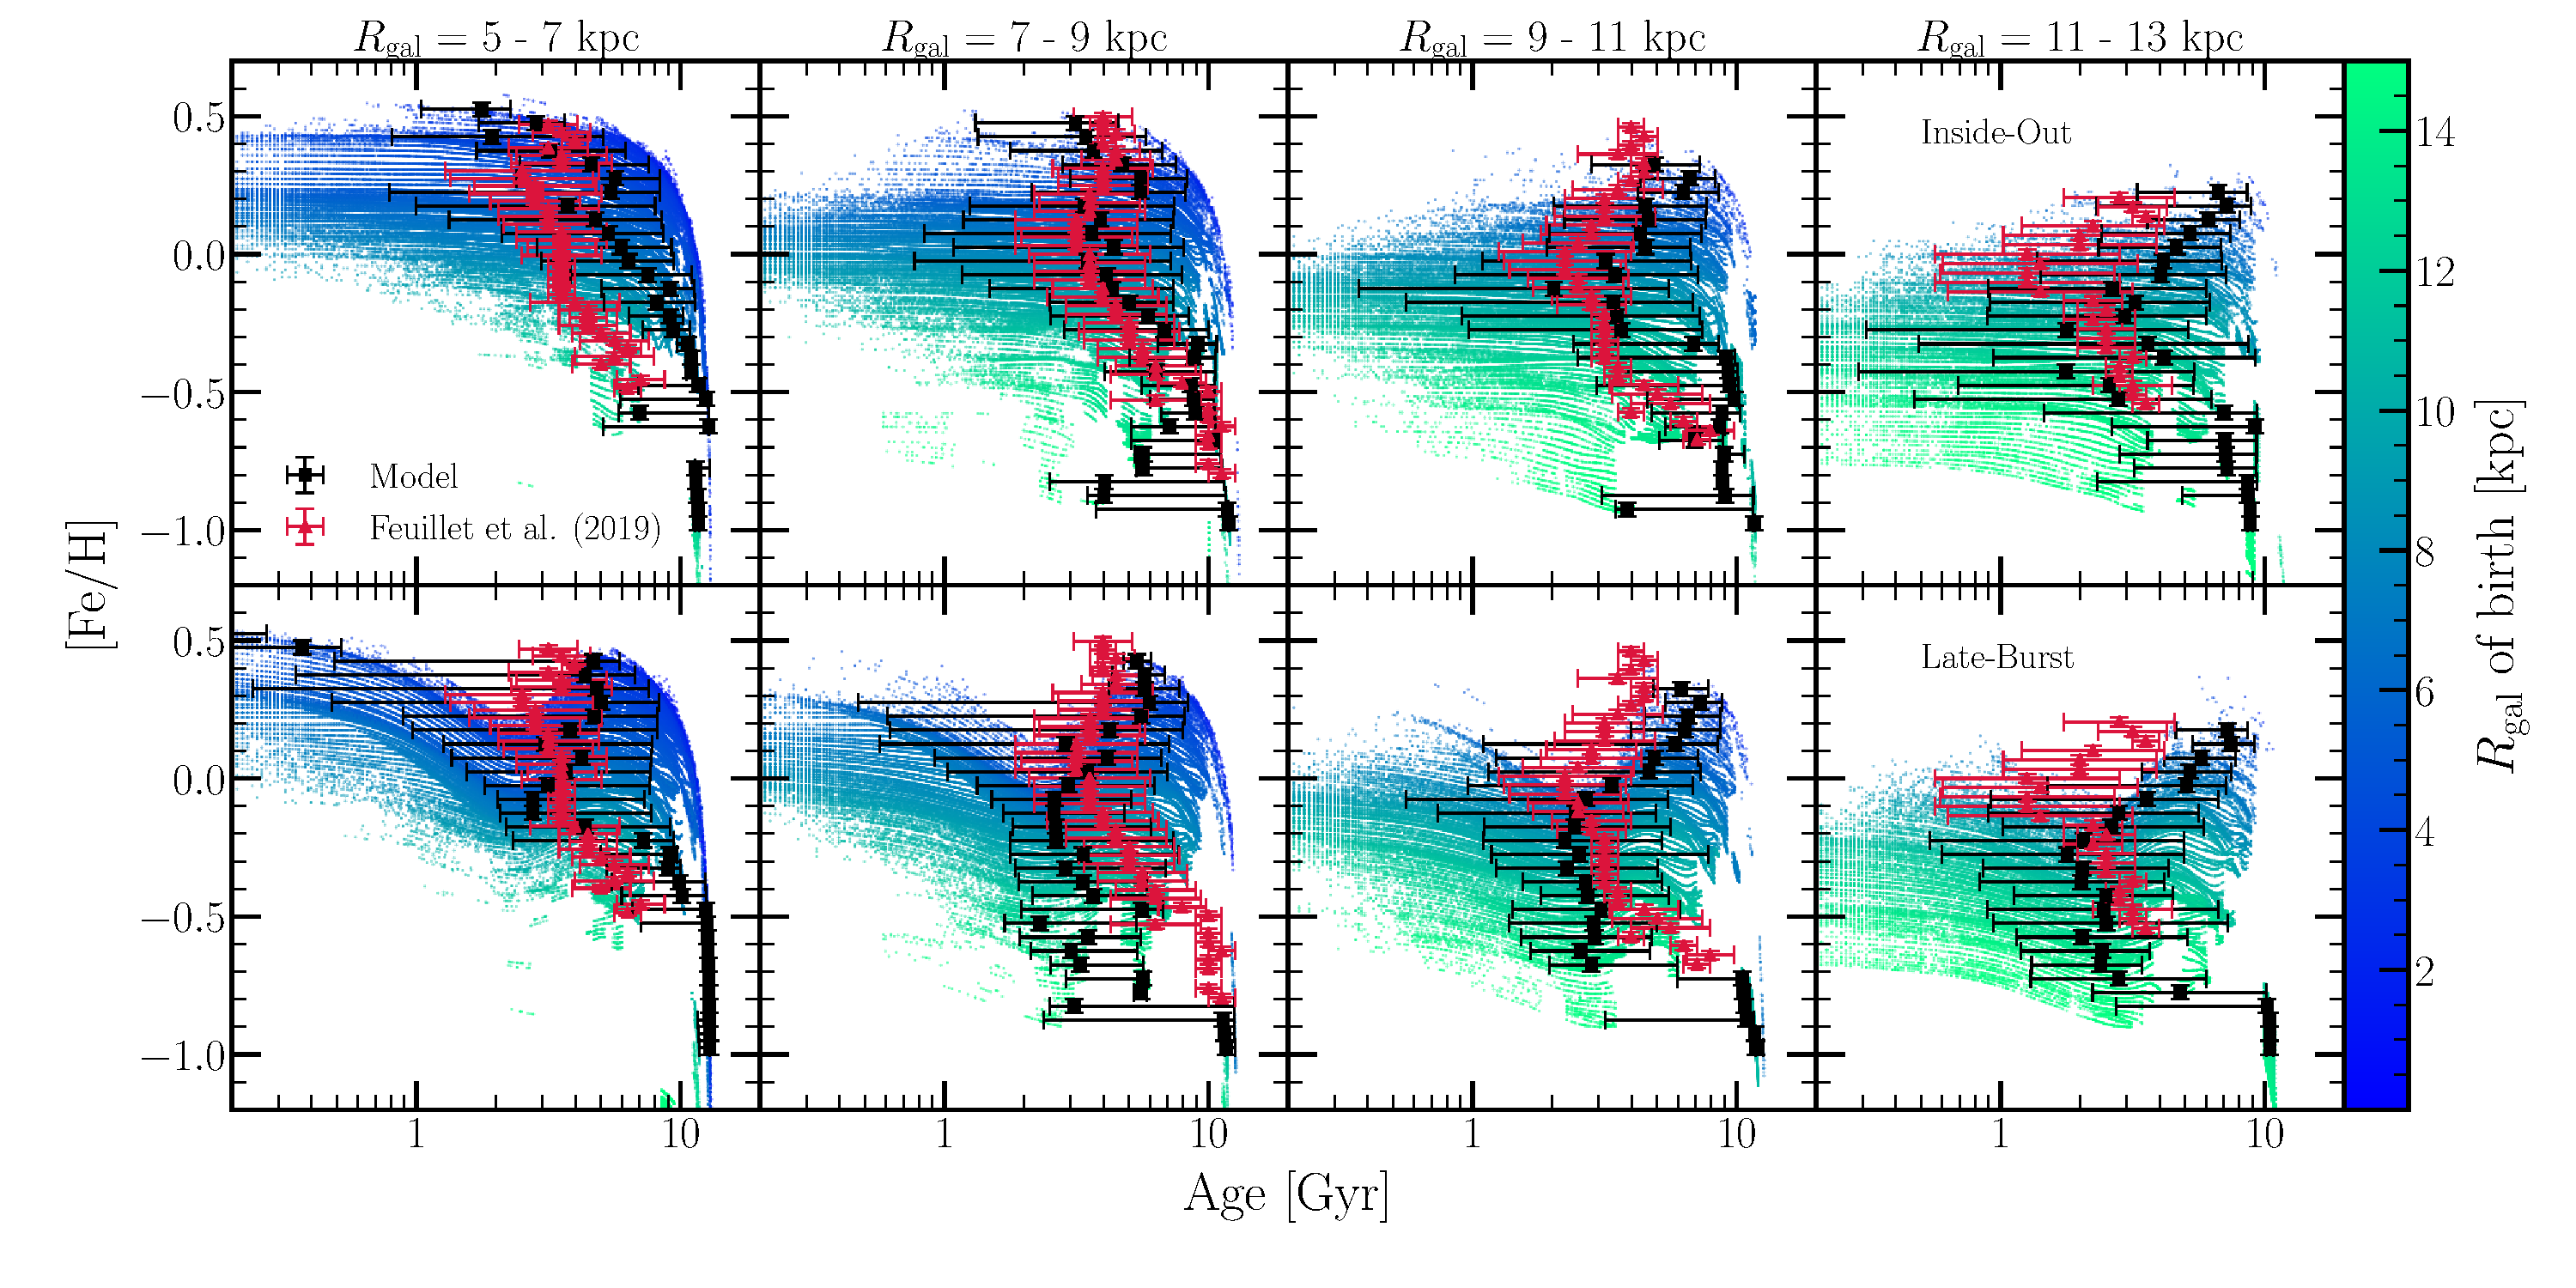
\includegraphics[scale = 0.35]{amr_insideout_vs_lateburst_fe.pdf} 
\caption{The age-[Fe/H] relation predicted by our inside-out (top) and 
late-burst (bottom) SFHs for~$R_\text{gal}$ = 5 - 7 kpc (left), 7 - 9 kpc 
(left middle), 9 - 11 kpc (right middle), and 11 - 13 kpc (right). Each panel 
shows only the~$\left|z\right|\leq$~0.5 kpc population. Red triangles, black 
squares, error bars, and coloured points are as in Fig.~\ref{fig:age_alpha} for 
the corresponding Galactic region, but with our model prediction quantified in 
bins of~$\Delta$[Fe/H] = 0.05. } 
\label{fig:amr_insideout_vs_lateburst_fe} 
\end{figure*} 

Motivated by this, we compare the predictions of the inside-out and late-burst 
SFH models to the~\citet{Feuillet2019} age-[Fe/H] relation in Fig. 
\ref{fig:amr_insideout_vs_lateburst_fe}. We retain the same plotting scheme 
used throughout this section and~\S~\ref{sec:obs_comp:age_alpha}, illustrating 
the inside-out model in the top row and the late-burst model in the bottom row. 
Each column corresponds to a specific range in~$R_\text{gal}$, denoted at the 
top of the figure. Beyond the solar annulus, we note that our inside-out model 
has a number of short-comings in comparison to the~\citet{Feuillet2019} 
measurements. At~$R_\text{gal}$ = 5 - 7 kpc, it overpredicts the characteristic 
ages of [Fe/H]~$\approx$~-0.3 - 0 stars. At~$R_\text{gal}$ = 9 - 11 and 11 - 13 
kpc, it mildly overpredicts ages at most abundances, and fails to reproduce the 
trend seen in the observed sample. The same can be said about the 
$R_\text{gal}$~=5 - 7 kpc region, and although the overall agreement is 
generally good there, one could reasonably argue this for the solar annulus as 
well. 
\par 
The late-burst model improves upon these shortcomings of the inside-out model 
considerably. At~$R_\text{gal}$ = 5 - 7 kpc, the overpredicted ages at solar 
and mildly sub-solar [Fe/H] is no longer present; this is also true at 
$R_\text{gal}$~= 9 - 11 and 11 - 13 kpc. Furthermore, the trend is much better 
reproduced at all radii in the late-burst than the inside-out model. The only 
different between the late-burst and inside-out model being the recent 
enhancement in the SFR, this is what drives the differences in model 
predictions. To fuel the starburst as we have parameterized it,~\texttt{VICE} 
calculates that there must be substantial gas accretion (see the infall rate 
$\dot{\Sigma}_\text{in}$ as a function of radius and time in Fig. 
\ref{fig:evol}). In our models, we assume accretion to always be of zero 
metallicity gas. As a result, the model predicts dilution of the ISM Fe 
abundance during the starburst; this can be seen by the trend of the coloured 
points in Fig.~\ref{fig:amr_insideout_vs_lateburst_fe} to lower [Fe/H] at ages 
of~$\sim$2 - 3 Gyr. At this time, the star formation rate is elevated by 
construction. The net effect is to increase the frequency of~$\sim$2 - 3 Gyr 
old stars with near- and sub-solar abundances globally, which lowers the 
characteristic ages of stars at these metallicities relative to the inside-out 
model. Using the~\citet{Feuillet2019} measurements as the observational 
benchmark, we favor the late-burst model here. 
\par 
Although there appears to be a vertical offset between the observed result and 
the model prediction at~$R_\text{gal}$ = 9 - 11 and 11 - 13 kpc, this is still 
an improvement upon the inside-out model. It's possible that this points to a 
need for higher yields of Fe than we've adopted here, though it's unclear if 
this would negatively affect the agreement at~$R_\text{gal}$~= 5 - 7 and 7 - 9 
kpc. It's possible that our parameterization of the mass-loading factor~$\eta$ 
scales too strongly with~$R_\text{gal}$ in the outer Galaxy (see discussion in 
\S~\ref{sec:methods:yields}). Alternatively, outflows in nature may be more 
efficient at removing some elements from the ISM than others; this could impact 
the overall normalization of the AMR at different radii. Our models in the 
present paper assume that outflows always proceed exactly at the metallicity of 
the ISM, but some authors argue that outflows can have a different metallicity 
- usually a higher one - due to containing in some part the metal-rich 
supernova ejecta that was added directly to the outflow by the explosions 
(observationally:~\citealp*{Chisholm2018}; in simulations: 
\citealp{Christensen2018}). 
\par 
We also note that the late-burst model predicts particularly young 
characteristic ages for the most metal-rich bins at~$R_\text{gal}$ = 5 - 7 kpc. 
This is purely a consequence of our choice to use the mass-weighted median as 
the population-averaged age measurement at fixed abundance. In this case, our 
model is simply reporting the 50th percentile of an age-distribution 
which is noticeably bimodal; as a result, whether or not the characteristic 
ages we report there are <1 Gyr or in better agreement with the 
\citet{Feuillet2019} measurements strongly depends on how we've parameterized 
the recent starburst as a function of both time and radius. Here we've made the 
simplest assumption of letting have the same time-dependence at all radii, 
which was not necessarily the case. 
\par 
Although we demonstrate here that the late-burst model describes the age-[Fe/H] 
relation reported by~\citet{Feuillet2019} better than the inside-out model, we 
found the exact opposite with regard to the age-[$\alpha$/Fe] relation with 
the same obesrvational sample in~\S~\ref{sec:obs_comp:age_alpha}. It's unlikely 
this discrepancy can be mitigated using any model which exhibits a recent 
starburst as parameterized here; as we demonstrated in~\S 
\ref{sec:obs_comp:age_alpha}, such models predict a global increase in 
[$\alpha$/Fe] due to the perturbed ratio of CCSN and SN Ia rates 
\citep{Johnson2020}, a feature which simply isn't seen in the 
\citet{Feuillet2019} measurements. It's possible that the Milky Way experienced 
dilution with no ensuing starburst - this would be the case if the majority of 
the accreted gas was warm, neutral and ionized gas which simply hasn't yet been 
made available for star formation. Such a scenario would exhibit some of the 
predictions of the late-burst model, but without the increase in [O/Fe] at late 
times, potentially allowing it to simultaneously explain the age-[$\alpha$/Fe] 
relation and AMR as they are observed. However, these models would be at odds 
with the findings of~\citet{Mor2019} and~\citet{Isern2019}. 
\par 
We remark that we find similar results for the age-[O/H] relation; furthermore, 
as in~\S~\ref{sec:obs_comp:age_alpha} for the age-[$\alpha$/Fe] relation, we 
also find for the age-[Fe/H] and age-[O/H] relations that our models tend to 
overpredict ages with increasing~$\left|z\right|$. Lastly, we caution future 
studies against basing the likelihood of a chemical evolution model on data 
for the solar annulus alone. In Fig.~\ref{fig:amr_solar_annulus}, we 
noted that there was decent agreement between the inside-out SFH model and 
the~\citet{Feuillet2019} measurements of the age-[O/H] and age-[Fe/H] 
relations in the solar annulus, but upon extending the comparison to other 
Galactic regions in Fig.~\ref{fig:amr_insideout_vs_lateburst_fe}, a number of 
shortcomings revealed themselves. Although to some extent this is made possible 
only recently with observational capabilities now allowing statistical 
measurements of these correlations for stars at greater distances from the sun, 
had we stopped there, we would have missed this interesting and peculiar 
result. 

\section{Discussion \& Conclusions} 
\label{sec:conclusions} 
In this paper, we have modeled the Milky Way as a series of concentric annuli 
with a~$\Delta R_\text{gal}$~= 100 pc width, describing each annulus as a 
conventional one-zone chemical evolution model and allowing the exchange of 
stellar populations between zones to include the impact of stellar migration in 
the model Galaxy. Though there have been a handful of studies which employ a 
similar methodology~\citep{Schoenrich2009, Nidever2015, Sharma2020}, ours and 
the~\citet{Minchev2013, Minchev2014, Minchev2017} model are the only ones which 
make use of a hydrodynamical simulation to describe radial mixing, for which we 
make use of the~\texttt{h277} zoom-in simulation~\citep{Christensen2012, 
Zolotov2012, Loebman2012, Loebman2014, Brooks2014}. This yields a model for 
migration which does not have any free parameters (see discussion in~\S 
\ref{sec:methods:h277}). 
\par 
Our model predicts masses and abundances for simple stellar populations, a 
given number of which form at each timestep. Each stellar 
population is then assigned a star particle from~\texttt{h277} which was born 
at a similar radius and time to act as an~\textit{analog}. The stellar 
population in our model then assumes the change in radius~$\Delta R_\text{gal}$ 
of the analog at face value, and is assumed to reside at the same present day 
height above/below the disc midplane~$\left|z\right|$. We then construct four 
models describing the time-dependence with which stellar populations move to 
their present-day radii, taking one in which radius changes with a 
$\sqrt{\text{age}}$-dependence in the fiducial model based on~\citet[][see 
Fig.~\ref{fig:migration_schema} and discussion in~\S 
\ref{sec:methods:migration}]{Frankel2018, Frankel2020}. 
\par 
We assume SN yields and a SN Ia delay-time distribution based on 
a combination of theoretical and empirical constraints. The main free 
parameters are the star formation law parameterizing the SFE timescale 
$\tau_\star$ (see discussion in~\S~\ref{sec:methods:sfe}), the mass-loading 
factor~$\eta(R_\text{gal})$~describing the strength of outflows (assumed to be 
time-independent; see discussion in~\S~\ref{sec:methods:yields}), and the SFH. 
The first we choose from the observed~$\dot{\Sigma}_\star - \Sigma_\text{g}$ 
relation in local spirals~\citep{Bigiel2010, Leroy2013, Krumholz2018}. The 
second is chosen to reproduce the metallicity gradient as observed 
\citep{Daflon2009, Frinchaboy2013, Hayden2014, Weinberg2019}. Our fiducial 
model then has an inside-out SFH with e-folding timescales calibrated to the 
\citet{Sanchez2020} data (see discussion in~\S~\ref{sec:methods:sfhs}). 
Motivated by the results of~\citet{Mor2019} and~\citet{Isern2019} suggesting 
such an evolutionary history, we construct models which exhibit a recent burst 
in star formation on top of the base-line model, as well as a constant SFH 
model of purely theoretical interest. 
\par 
We find that when stellar migration proceeds in a manner in which a star's 
orbital radius changes continuously with time, the SN Ia rate as a function of 
both radius and time exhibits significant variability. The characteristic delay 
time of a single SN Ia event is~$\sim$1 Gyr~\citep{Maoz2012, Maoz2017}, and 
stars are migrating a significant distance in the radial direction on similar 
timescales in our models. The result is a SN Ia rate which, at fixed radius, 
tends to follow that which is expected from the SFH when averaged with time, 
but whose instantaneous value may be considerably larger or smaller. Our model 
predicts the amplitude of this variability to grow with increasing radius due 
to sampling noise and the inverse dependence of the stellar surface density on 
$R_\text{gal}$. We demonstrate that this is a mechamism with which truly young, 
super-solar [$\alpha$/Fe] stars can form. When the SN Ia rate increases or 
decreases, the Fe abundance in the ISM increases or 
decreases accordingly; this in turn affects the gas-phase [$\alpha$/Fe] ratio, 
and the stars which form at these times inherit these compositions. Of the 
young stars, those with the highest [$\alpha$/Fe] form at large~$R_\text{gal}$ 
($\gtrsim$~12 kpc) due to the radial dependence of the amplitude; a subsample 
of these stars can then migrate to the solar annulus. 
\par 
To our knowledge, this mechanism lends the first theoretical explanation of 
truly young $\alpha$-rich stars in the solar neighbourhood, revealed recently 
by the observations of the APOGEE survey~\citep{Martig2016, Feuillet2018, 
Feuillet2019, SilvaAguirre2018}.~\citet{SilvaAguirre2018} find that 
these stars have kinematics consistent with the rest of the high-$\alpha$ 
population, and postulate based on this that these stars are the consequence 
of stellar mergers or mass transfer events, making truly old stars simply 
appear younger. In a sample of 51 young~$\alpha$-rich red giants, 
\citet{Hekker2019} demonstrate using cabon-to-nitrogen ratios that a portion of 
these stars are indeed old, but that these effects cannot account for the 
entire population. We argue based on our results that the truly young ones 
formed at large~$R_\text{gal}$~at a time when the ISM was intrinsically 
$\alpha$-rich due simply to a deficit in SN Ia events caused by a net loss of 
white dwarf progenitors to stellar migration. We remark that our model would 
sugest that these stars have super-solar [$\alpha$/Fe] not because they are 
$\alpha$-rich, but rather that they are Fe-poor. 
\par 
We find that our model adequately reproduces the variations in MDFs with 
Galactocentric radius in the disc~\citep{Hayden2015}. Although there is a 
potential for improved agreement in the~$R_\text{gal}$~= 3 - 5 kpc bin, the 
model nonetheless performs well. With increasing~$\left|z\right|$, the 
prediction breaks down somewhat. Where the observational data show a 
convergence of the MDFs at all radii to a skew-positive distribution with 
mode([O/H])~$\approx$~mode([Fe/H])~$\approx$~-0.5, our model predicts the mode 
abundance in the inner Galaxy to decrease slightly, though not to the same 
extent as in the observations, while the distributions at larger~$R_\text{gal}$ 
are less affected (see Figs.~\ref{fig:mdf_3panel_fe} and~\ref{fig:mdf_3panel_o} 
and discussion in~\S~\ref{sec:obs_comp:mdfs}). While the model accounts for a 
portion of these effects, it cannot explain the entire~$z$-dependence of the 
MDF shape. 
\par 
We demonstrate the dependence of the relative frequency of high-$\alpha$ and 
low-$\alpha$ sequence stars on Galactic position (see, e.g., Fig. 4 of 
\citealp{Hayden2015}) is at least in part a consequence of stellar migration. 
In our fiducial inside-out SFH model, low [Fe/H], high [$\alpha$/Fe] stars 
are the dominant population at small~$R_\text{gal}$~and high~$\left|z\right|$; 
conversely, low [$\alpha$/Fe] stars are most common at large~$R_\text{gal}$ 
and low~$\left|z\right|$. We clarify that this is not an explanation for the 
\textit{origin} of the two sequences - only the spatial dependence thereof. 
In fact, our model is unable to account for the presence of the infamous 
[$\alpha$/Fe] dichotomy in any of the variants we've explored. While it is able 
to reproduce the broad nature of the [O/Fe] distributions at fixed [Fe/H] and 
may show a convincing two-peaked profile in a specific Galactic region, it 
fails to do so for the entire Galaxy at all metallicities; the principle 
failure is an overpredicted frequency of intermediate [$\alpha$/Fe] stars. This 
is in contrast to the findings of~\citet{Sharma2020}, who claim to reproduce 
the bimodality in a model assuming an inside-out SFH with stellar migration. 
However, they do not demonstrate that the enrichment history of their model 
follows self-consistently from their assumed SFH. We therefore argue that 
an inside-out SFH is not conducive to forming the abundance distributions 
observed in the Milky Way. Though we don't investigate such evolutionary 
pathways in the present paper, our models fail in such a manner that suggests 
the agreement can best be improved by the three-phase SFH of the two-infall 
model~\citep{Chiappini1997, Chiappini2001, Romano2010, Grisoni2017, 
Noguchi2018, Palla2020, Spitoni2016, Spitoni2018, Spitoni2019a, Spitoni2020, 
Spitoni2021}. We reserve an investigation into more sophisticated forms of the 
Galactic SFH for future work. 
\par 
We find that the age-[O/Fe] relation as reported by~\citet{Feuillet2019} is 
well-characterized by our inside-out SFH. In the case of our recent 
starburst models motivated by~\citet{Mor2019} and~\citet{Isern2019}, the 
elevation of the SFR necessitates an increase in [$\alpha$/Fe] for young 
stars owing to the increased rate of CCSNe before the onset of SN Ia associated 
with the starburst~\citep{Johnson2020}, introducing a trend which simply isn't 
seen in the observations. This suggests that recent studies finding an 
elevation in the 
Galactic SFR~$\sim$2 Gyr ago are at odds with chemical evolution models, which 
based on the monotonic nature of the observed AMR would put constraints on the 
amount of variability out to lookback times of~$\sim$8 Gyr. Lastly, we find 
that our model predicts the intrinsic scatter in the age-[$\alpha$/Fe] relation 
to increase with~$R_\text{gal}$; this traces back to the variability in the SN 
Ia rates having a higher amplitude in the outer Galaxy, which produces an 
in-situ population with a larger dynamic range in [O/Fe]. 
\par 
We find that the AMR (both age-[O/H] and age-[Fe/H]) in the solar annulus as 
measured by~\citet{Feuillet2019} is well-described by our inside-out SFH. 
However, when this comparison is extended to other Galactic regions, the 
inside-out model overpredicts ages in multiple regions and fails to reproduce 
the population-averaged trend throughout the disc. We demonstrate that our 
late-burst model can account for these discrepancies, suggesting that the 
observed AMR favors a model with a recent enhancement in the Galactic SFR. 
Somewhat confusingly, the impact of the late-burst model is such that it is 
convincingly rejected by the age-[O/Fe] relation but convincingly favored by 
the age-[O/H] and age-[Fe/H] relations. 
\par 
We thus conclude that no single model in the present paper can explain all of 
the observables of interest here. This suggests that 
conventional assumptions about the evolution of the Milky Way, such as an 
inside-out SFH with stellar migration, are not sufficiently accurate to 
understand the enrichment history of the Milky Way in detail. This is an 
indication that at present there is more astrophysical information in already 
collected observations than the most recent GCE models can explain. It's likely 
our models are missing at least one key component with a significant impact on 
the predicted abundances. 
\par 
Lastly, we remark on the low number of multi-zone chemical evolution models in 
the literature, some with and some without migration. In this paper, we present 
only a handful of models whose predictions can be calculated with a combined 
CPU-time comparable to a single working day. These models make straight-forward 
predictions which can easily be compared to publicly-available observed data. 
Though they are extremely useful in many respects, these medium resolution, 
medium computational expense techniques can test assumptions about the 
evolutionary history of the Milky Way with more control over the parameters and 
much less computational expense than the higher overhead hydrodynamical 
simulations; our models here constitute an example of a combination of the two. 
\par 
\texttt{VICE} is publicly available and open-source;\footnote{
	Install (PyPI): \url{https://pypi.org/project/vice} \\ 
	Documentation: \url{https://vice-astro.readthedocs.io} \\ 
	Source Code: \url{https://github.com/giganano/VICE.git} 
} it can be installed in a~\texttt{Unix} terminal via~\texttt{pip install vice}. 
\texttt{Python} code which runs the simulations presented in this paper is 
included as supplementary material in the~\texttt{GitHub} repository; our 
models can be ran directly from a terminal without modifying the source code, 
and are capable of predicting abundances for~$\sim$2 million stellar 
populations in~$\sim$2.5 CPU-hours running on a single core on personal 
computers. 

\section{Acknowledgements} 
\label{sec:acknowledgements} 
We acknowledge valuable discussion with, in no particular order, Emily 
Griffith, Jennifer Johnson, Todd Thompson, Jiayi Sun, Amy Sardone, Adam Leroy, 
Grace Olivier, the Ohio State Astronomy Gas, Galaxies, and Feedback group, and 
various participants of the SDSS Gotham 2020 virtual collaboration meeting and 
the virtual 236th meeting of the American Astronomical Society. This work was 
supported in part by National Science Foundation grant AST-1909841. D.H.W. 
is grateful for the hospitality of the Institute for Advanced Study and the 
support of the W.M. Keck Foundation. 
\par 
In this paper we have made use of data from SDSS-IV APOGEE-2 DR16. 
Funding for the Sloan Digital Sky 
Survey IV has been provided by the 
Alfred P. Sloan Foundation, the U.S. 
Department of Energy Office of 
Science, and the Participating 
Institutions. 
\par 
SDSS-IV acknowledges support and 
resources from the Center for High 
Performance Computing  at the 
University of Utah. The SDSS 
website is~\url{www.sdss.org}.
\par 
SDSS-IV is managed by the 
Astrophysical Research Consortium 
for the Participating Institutions 
of the SDSS Collaboration including 
the Brazilian Participation Group, 
the Carnegie Institution for Science, 
Carnegie Mellon University, Center for 
Astrophysics | Harvard \& 
Smithsonian, the Chilean Participation 
Group, the French Participation Group, 
Instituto de Astrof\'isica de 
Canarias, The Johns Hopkins 
University, Kavli Institute for the 
Physics and Mathematics of the 
Universe (IPMU) / University of 
Tokyo, the Korean Participation Group, 
Lawrence Berkeley National Laboratory, 
Leibniz Institut f\"ur Astrophysik 
Potsdam (AIP),  Max-Planck-Institut 
f\"ur Astronomie (MPIA Heidelberg), 
Max-Planck-Institut f\"ur 
Astrophysik (MPA Garching), 
Max-Planck-Institut f\"ur 
Extraterrestrische Physik (MPE), 
National Astronomical Observatories of 
China, New Mexico State University, 
New York University, University of 
Notre Dame, Observat\'ario 
Nacional / MCTI, The Ohio State 
University, Pennsylvania State 
University, Shanghai 
Astronomical Observatory, United 
Kingdom Participation Group, 
Universidad Nacional Aut\'onoma 
de M\'exico, University of Arizona, 
University of Colorado Boulder, 
University of Oxford, University of 
Portsmouth, University of Utah, 
University of Virginia, University 
of Washington, University of 
Wisconsin, Vanderbilt University, 
and Yale University.

\textit{Software}: Matplotlib~\citep{Matplotlib}; Astropy~\citep{Astropy2013, 
Astropy2018}; NumPy~\citep{NumPy}. 

\section{Data Availability} 
\label{sec:data_availability} 
\texttt{VICE} is open-source software, and the code which computes abundances 
for our models is publicly available as well. In the GitHub repository, we 
provide detailed instructions on how to run our models and variations thereof. 
All observational data appearing in this paper is publicly available, and is 
also included with the source code for our models and figures. 

\begin{appendices} 

\section{Normalizing the Star Formation History} 
\label{sec:normalize_sfh} 
In this appendix, we derive a prescription for calculating the prefactors of an 
adopted star formation history (SFH) for each annulus in our models. As 
mentioned in~\S~\ref{sec:methods:sfhs}, this procedure requires a unitless 
description of the time-dependence of the SFH in each annulus, denoted 
$f(t|R_\text{gal})$, and a unitless description denoting the radial dependence 
of the stellar surface density~$g(R_\text{gal})$. By additionally selecting a 
total stellar mass of the present day model Galaxy, the solution to the 
detailed form of the star formation history 
$\dot{\Sigma}_\star(t, R_\text{gal})$ is unique. With this approach, we assume 
that stellar migration does not significantly impact the form of 
$g(R_\text{gal})$, an assumption we demonstrate to be accurate in~\S 
\ref{sec:methods:surface_density_gradient}. 
\par 
The surface density of star formation with units of mass per area per time can 
be expressed in terms of~$f(t|R_\text{gal})$ as: 
\begin{equation} 
\dot{\Sigma}_\star(t, R_\text{gal}) = \dot{\Sigma}_\star(t = 0, R_\text{gal}) 
f(t|R_\text{gal}) 
\label{eq:sfh_terms_of_f} 
\end{equation} 
and the present-day radial surface density gradient with units of mass per area 
as: 
\begin{equation} 
\Sigma_\star(R_\text{gal}) = \Sigma_\star(R_\text{gal} = 0) g(R_\text{gal}) 
\label{eq:sigma_terms_of_g}  
\end{equation} 
The integral of~$\dot{\Sigma}_\star$ with time should yield the surface density 
gradient at a given radius~$R_\text{gal}$, up to a prefactor accounting for the 
return of stellar envelopes to the interstellar medium (ISM): 
\begin{subequations}\begin{align} 
\Sigma_\star(R_\text{gal}) &= (1 - r)\int_0^T \dot{\Sigma}_\star(t, 
R_\text{gal}) dt 
\\ 
&= (1 - r) \dot{\Sigma}_\star(t = 0, R_\text{gal})\int_0^T f(t|R_\text{gal}) dt 
\\ 
\dot{\Sigma}_\star(t = 0, R_\text{gal}) &= \Sigma_\star(R_\text{gal}) 
\left[(1 - r) \int_0^T f(t|R_\text{gal})dt\right]^{-1} 
\\ 
&= \Sigma_\star(R_\text{gal} = 0)g(R_\text{gal}) \left[(1 - r) \int_0^T 
f(t|R_\text{gal})\right]^{-1} 
\label{eq:intermediate_1} 
\end{align}\end{subequations} 
where~$(1 - r) \approx 0.6$~is an adequate approximation for a 
\citetalias{Kroupa2001} IMF~\citep[][see discussion in their~\S 
2.2]{Weinberg2017}. This expression relates the two unkowns introduced by 
equations~\refp{eq:sfh_terms_of_f} and~\refp{eq:sigma_terms_of_g}. We continue 
by asserting that the integral of the stellar surface density over the area of 
the disc should be equal to the present-day stellar mass of the Milky Way: 
\begin{subequations}\begin{align} 
M_\star^\text{MW} &= \int_0^R \Sigma_\star(R_\text{gal}) 2\pi R_\text{gal} 
dR_\text{gal} 
\\ 
&= \Sigma_\star(R_\text{gal} = 0) \int_0^R g(R_\text{gal}) 2\pi R_\text{gal} 
dR_\text{gal} 
\\ 
\Sigma_\star(R_\text{gal} = 0) &= M_\star^\text{MW} \left[\int_0^R 
g(R_\text{gal}) 2\pi R_\text{gal}dR_\text{gal}\right]^{-1} 
\label{eq:intermediate_2} 
\end{align}\end{subequations} 
\par 
Now plugging equation~\refp{eq:intermediate_2} into equation 
\refp{eq:intermediate_1}, and then that into equation~\refp{eq:sfh_terms_of_f} 
yields the desired result: 
\begin{subequations}\begin{align} 
&\dot{\Sigma}_\star(t, R_\text{gal}) = Af(t|R_\text{gal})g(R_\text{gal}) 
\\ 
&A = M_\star^\text{MW}\left[(1 - r) \int_0^R g(R_\text{gal})2\pi R_\text{gal} 
dR_\text{gal} \int_0^T f(t|R_\text{gal})dt\right]^{-1} 
\end{align}\end{subequations} 
where the upper limits should be the maximum radius of star formation and the 
end time of the simulation (15.5 kpc and 12.2 Gyr in this paper). This result 
makes intuitive sense, simply stating that the required normalization of 
$f(t|R_\text{gal})$~is specified by two things: the total stellar mass of the 
Galaxy and how steep the stellar density falls with increasing radius. As long 
as the assumption that stellar migration does not significantly alter the form 
of~$g(R_\text{gal})$~is not violated, this procedure can be used to calculate 
prefactors for future models of disc galaxies. 

\end{appendices} 

\bibliographystyle{mnras} 
\bibliography{draft1} 

\label{lastpage} 
\end{document} 

